\chapter{双曲型问题}\label{ch:14}
\SourcePage{457}

双曲型方程的数值逼近是一个十分活跃的研究领域.这类初边值问题最显著的特点是扰动以有限速度传播.另一个特点是,边界处理比椭圆型或抛物型方程复杂.方程系数的符号决定哪些边界区域是流入边界、哪些是流出边界,从而决定各具体问题应在何处给定边界条件.对于双曲型方程组,情形更复杂,需要在边界处作局部特征分析.数值实现不当的边界条件可能引起非物理的不稳定.

双曲型问题还可能出现间断解.间断既可能由非线性方程产生,也可能出现在初始数据有间断的线性问题中.为了容纳不光滑解,可以把问题改写为弱形式,使空间导数只作用在光滑的试验函数上.大体说来,有限差分和配置逼近都直接从方程的微分形式导出.Galerkin 法,包括有限元和谱方法,则从弱形式出发.第三种方法是有限体积法,尤其常用于双曲型守恒律方程组.它从方程的积分形式导出,将积分限制在计算区域的各个子区域内,这些子区域称为控制体积.这样便可保证各个控制体积内的守恒.

本章主要讨论线性和非线性方程的有限差分格式.第~\BookRef{sec:14.1}{14.1}~节先介绍几个有代表性的双曲型方程及其主要数学性质,第~\BookRef{sec:14.2}{14.2}~节再讨论有限差分格式.第~\BookRef{sec:14.3}{14.3}~节和第~\BookRef{sec:14.4}{14.4}~节分别简要介绍有限元逼近和谱逼近.第~\BookRef{sec:14.5}{14.5}~节简述波动方程及其有限元逼近.最后,第~\BookRef{sec:14.6}{14.6}~节讨论有限体积法.

\section{双曲型方程的若干实例}\label{sec:14.1}
\SourcePage{458}

先考察几个双曲型初值问题和初边值问题的例子.

\subsection{线性标量对流方程}\label{sec:14.1.1}

\begin{example}[线性对流方程]\label{ex:14.1.advection}
最简单的双曲型方程是线性对流方程
\begin{equation}\label{eq:14.1.1}
  \frac{\partial u}{\partial t}+a\frac{\partial u}{\partial x}=0,
      \qquad t>0,\quad x\in\mathbb R,
\end{equation}
其中 \(a\in\mathbb R\setminus\{0\}\).方程\eqref{eq:14.1.1}与初始条件
\begin{equation}\label{eq:14.1.2}
  u(0,x)=u_0(x),\qquad x\in\mathbb R
\end{equation}
构成的 Cauchy 问题,其解就是速度为 \(a\) 的行波：
\[
  u(t,x)=u_0(x-at),\qquad t\ge0.
\]
解沿\emph{特征线}保持常值.特征线是在 \((t,x)\) 平面上满足下列常微分方程的曲线 \(X(t)\)：
\[
  \begin{cases}
    X'(t)=a, & t>0,\\
    X(0)=x_0.
  \end{cases}
\]
\end{example}

更一般地,考虑
\begin{equation}\label{eq:14.1.3}
  \frac{\partial u}{\partial t}+a\frac{\partial u}{\partial x}+a_0u=f,
     \qquad t>0,\quad x\in\mathbb R,
\end{equation}
其中 \(a,a_0,f\) 是给定的 \((t,x)\) 的函数.仍以如下方程的解 \(X(t)\) 定义特征线：
\begin{equation}\label{eq:14.1.4}
  \begin{cases}
    X'(t)=a(t,X(t)), & t>0,\\
    X(0)=x_0.
  \end{cases}
\end{equation}
这时,\eqref{eq:14.1.3}的解满足
\[
  \frac{d}{dt}u(t,X(t))=f(t,X(t))-a_0(t,X(t))u(t,X(t)).
\]
解沿特征线随时间变化,一般也没有简单的表达式.不过,求解两组常微分方程即可得到它.因此,如果 \(a,a_0,f,u_0\) 光滑,且 \(a\) 的增长使特征线可延拓到任意有限时间,那么对所有 \(t>0\),光滑解都存在.

\SourcePage{459}
回到方程\eqref{eq:14.1.1}.上面的推导假定 \(u\) 光滑,以便使用一阶导数.初始数据不光滑的情形也能处理.从上面的推导容易推测,若 \(u_0\) 在某一点 \(x_0\) 处有间断,这个间断就沿从 \(x_0\) 出发的特征线传播.引入双曲型方程的弱解之后,便可赋予这一过程确切的数学含义.

例如,以一列光滑函数 \(u_0^\varepsilon(x)\)(\(\varepsilon>0\))逼近初值 \(u_0(x)\),即可把非光滑情形转化为光滑情形.问题\eqref{eq:14.1.1}对光滑初值的解为 \(u^\varepsilon(t,x)=u_0^\varepsilon(x-at)\),其中 \(t\ge0\),\(x\in\mathbb R\).设 \(\|u_0-u_0^\varepsilon\|_{L^1(\mathbb R)}\le\varepsilon\),这里
\begin{equation}\label{eq:14.1.5}
  \|v\|_{L^1(\mathbb R)}:=\int_{-\infty}^{\infty}|v(x)|\,\mathrm dx
\end{equation}
是 \(L^1\) 范数,则
\[
  \lim_{\varepsilon\to0}u^\varepsilon(t,x)
    =\lim_{\varepsilon\to0}u_0^\varepsilon(x-at)=u_0(x-at),
\]
其中对每个 \(t\ge0\),极限均在 \(L^1\) 范数下取.

非线性双曲型方程即使从光滑初值出发也可能形成奇性,因此只光滑化初值并不能解决困难.另一种做法是将方程\eqref{eq:14.1.1}正则化,即对充分小的 \(\varepsilon>0\),用\emph{抛物型}对流--扩散方程
\[
  \frac{\partial u^\varepsilon}{\partial t}
    +a\frac{\partial u^\varepsilon}{\partial x}
    =\varepsilon\frac{\partial^2u^\varepsilon}{\partial x^2},
    \qquad t>0,\quad x\in\mathbb R
\]
代替原方程.
\begin{definition*}
极限函数 \(\lim_{\varepsilon\to0}u^\varepsilon(t,x)\) 称为{\heiti 消失黏性解}.在这里它等于 \(u_0(x-at)\).
\end{definition*}
这一做法也可推广到非线性方程.不过,在有限空间区间上研究\eqref{eq:14.1.1}时,作为逼近的对流--扩散方程需要补充一个边界条件,且必须选得恰当,以免出现非物理的边界层.见第~\ref{ch:8}~章和第~\ref{ch:12}~章.

\subsection{线性双曲型方程组}\label{sec:14.1.2}

现在考虑形如
\begin{equation}\label{eq:14.1.6}
  \frac{\partial\boldsymbol{U}}{\partial t}+A\frac{\partial\boldsymbol{U}}{\partial x}=0,
     \qquad t>0,\quad x\in\mathbb R
\end{equation}
的线性方程组,其中 \(\boldsymbol{U}\colon[0,\infty)\times\mathbb R\to\mathbb R^p\),\(A\in\mathbb R^{p\times p}\) 为常矩阵.
\begin{definition*}
如果 \(A\) 可对角化,且特征值全为实数,就称这一方程组为{\heiti 双曲型}.
\end{definition*}
此时可作分解
\begin{equation}\label{eq:14.1.7}
  A=T\Lambda T^{-1},
\end{equation}
\SourcePage{460}
其中 \(\Lambda:=\operatorname{diag}(\lambda_1,\ldots,\lambda_p)\) 是以特征值为对角元的矩阵,\(T:=(\boldsymbol{\omega}^1|\boldsymbol{\omega}^2|\cdots|\boldsymbol{\omega}^p)\) 是以右特征向量为列的矩阵,即
\[
  A\boldsymbol{\omega}^k=\lambda_k\boldsymbol{\omega}^k,\qquad k=1,\ldots,p.
\]
假定 \(\lambda_1,\ldots,\lambda_{p_0}\) 非负,\(\lambda_{p_0+1},\ldots,\lambda_p\) 为负.若各特征值互不相同,则方程组为\emph{严格双曲型}.

在\eqref{eq:14.1.6}中引入\emph{特征变量} \(\boldsymbol{W}:=T^{-1}\boldsymbol{U}\),得到
\begin{equation}\label{eq:14.1.8}
  \frac{\partial\boldsymbol{W}}{\partial t}
    +\Lambda\frac{\partial\boldsymbol{W}}{\partial x}=0.
\end{equation}
这就解耦为 \(p\) 个彼此独立的标量对流方程
\begin{equation}\label{eq:14.1.9}
  \frac{\partial W_k}{\partial t}+\lambda_k\frac{\partial W_k}{\partial x}=0,
    \qquad k=1,\ldots,p,
\end{equation}
其解为 \(W_k(t,x)=W_k(0,x-\lambda_kt)\).所以,初值问题\eqref{eq:14.1.6}的解 \(\boldsymbol{U}=T\boldsymbol{W}\) 可以表示为
\begin{equation}\label{eq:14.1.10}
  \boldsymbol{U}(t,x)=\sum_{k=1}^pW_k(0,x-\lambda_kt)\boldsymbol{\omega}^k.
\end{equation}

在 \((t,x)\) 平面上,满足 \(X'(t)=\lambda_k\) 的曲线 \(X(t)=x_0+\lambda_kt\) 称为第 \(k\) 族特征线.特征变量 \(W_k\) 沿每条第 \(k\) 族特征线保持常值.对于严格双曲型方程组,\((t,x)\) 平面上每一点都通过 \(p\) 条互异的特征线.因此,任给 \(\bar t\) 和 \(\bar x\),\(\boldsymbol{U}(\bar t,\bar x)\) 只依赖于 \(p\) 个点 \(\bar x-\lambda_k\bar t\) 处的初始数据.
\begin{definition*}
从点 \((\bar t,\bar x)\) 向初始时刻回溯,各条特征线的足点构成集合
\begin{equation}\label{eq:14.1.11}
  D(\bar t,\bar x):=\{x\in\mathbb R\mid x=\bar x-\lambda_k\bar t,\ k=1,\ldots,p\}.
\end{equation}
这个集合称为解 \(\boldsymbol{U}\) 在点 \((\bar t,\bar x)\) 的{\heiti 依赖域}.
\end{definition*}

\begin{example}[波动方程]\label{ex:14.1.wave}
双曲型方程的一个经典例子是二阶\emph{波动方程}
\begin{equation}\label{eq:14.1.12}
  \frac{\partial^2u}{\partial t^2}=\gamma^2\frac{\partial^2u}{\partial x^2},
  \qquad t>0,\quad x\in\mathbb R,
\end{equation}
其中 \(\gamma>0\),初始数据为
\begin{equation}\label{eq:14.1.13}
  u(0,x)=u_0(x),\qquad \frac{\partial u}{\partial t}(0,x)=v_0(x).
\end{equation}
作变量变换
\begin{equation}\label{eq:14.1.14}
  U_1:=\frac{\partial u}{\partial x},\qquad U_2:=\frac{\partial u}{\partial t},
\end{equation}
便可从\eqref{eq:14.1.12}得到形如\eqref{eq:14.1.6}的一阶方程组,其中
\SourcePage{461}
\begin{equation}\label{eq:14.1.15}
  \boldsymbol{U}=(U_1,U_2),\qquad
  A=\begin{pmatrix}0&-1\\-\gamma^2&0\end{pmatrix},
\end{equation}
初始条件为 \(U_1(0,x)=u_0'(x)\) 和 \(U_2(0,x)=v_0(x)\).

矩阵 \(A\) 的特征值是两个互异的实数 \(\pm\gamma\),也就是波速,因此方程组是双曲型的.求出 \(A\) 的特征向量后,按对\eqref{eq:14.1.6}所用的对角化方法,可以得到解的两个分量 \(U_1,U_2\)：
\[
  \begin{aligned}
    U_1(t,x)&=\tfrac12\bigl[u_0'(\xi)+\gamma^{-1}v_0(\xi)
                 +u_0'(\eta)-\gamma^{-1}v_0(\eta)\bigr],\\
    U_2(t,x)&=\tfrac12[\gamma u_0'(\xi)+v_0(\xi)-\gamma u_0'(\eta)+v_0(\eta)],
  \end{aligned}
\]
其中 \(\xi:=x+\gamma t\),\(\eta:=x-\gamma t\).再由\eqref{eq:14.1.14}即可求得 \(u(t,x)\).

和前面一样,光滑的初始数据给出光滑解,初始数据中的奇性只能沿特征线传播.
\end{example}

\subsection{初边值问题}\label{sec:14.1.3}

现在考虑初边值问题,因而把前面各个双曲型方程的空间区域从整个实轴换成有限区间,例如 \(x\in I=(0,1)\).这时须根据问题的性质给定相容的边界数据.

对于对流方程\eqref{eq:14.1.1},边界条件取如下形式：
\begin{equation}\label{eq:14.1.16}
  \begin{cases}
    u(t,0)=\varphi_-(t), & a>0,\\
    u(t,1)=\varphi_+(t), & a<0,
  \end{cases}
\end{equation}
其中 \(\varphi_\pm(t)\) 是给定函数.若 \(a>0\),端点 \(x=0\) 是\emph{流入点},\(x=1\) 是\emph{流出点}.若 \(a<0\),两者的作用互换.同样,对于更一般的对流方程\eqref{eq:14.1.3},必须在所有流入边界点给定解 \(u\).根据 \(a(t,x)\) 在端点的符号,流入点可能有一个、两个,也可能没有.

相应初边值问题的解满足 \(L^2\) 范数下的先验界.事实上,以 \(u\) 乘\eqref{eq:14.1.3},将 \(x\) 从 \(0\) 积分到 \(1\),并对对流项分部积分,得到对每个 \(t>0\),
\[
  \begin{aligned}
    &\frac12\frac{d}{dt}\|u(t)\|_{0,I}^2+\int_0^1\mu(t,x)u^2(t,x)\,\mathrm dx\\
    &\quad=\int_0^1f(t,x)u(t,x)\,\mathrm dx
          +\tfrac12[-a(t,1)u^2(t,1)+a(t,0)u^2(t,0)],
  \end{aligned}
\]
\SourcePage{462}
其中采用通常的 \(L^2\) 范数记号(见第~\ref{sec:1.2}~节),并令
\[
  \mu(t,x):=a_0(t,x)-\tfrac12\frac{\partial a}{\partial x}(t,x).
\]
定义
\[
  \Phi(t):=-\sigma_+(t)a(t,1)\varphi_+^2(t)+\sigma_-(t)a(t,0)\varphi_-^2(t),
\]
其中
\[
  \sigma_+(t):=\begin{cases}1,&a(t,1)<0,\\0,&\text{其他情形},\end{cases}
  \qquad
  \sigma_-(t):=\begin{cases}1,&a(t,0)>0,\\0,&\text{其他情形}.\end{cases}
\]
立即有 \(\Phi(t)\ge0\),且
\[
  -a(t,1)u^2(t,1)+a(t,0)u^2(t,0)\le\Phi(t)\qquad\forall t>0.
\]
因此,利用 Gronwall 引理(见引理~\ref{lem:1.4.1}),对每个 \(t\in[0,T]\) 得到
\[
  \begin{aligned}
    \|u(t)\|_{0,I}^2
      &\le\biggl(\|u_0\|_{0,I}^2+\int_0^t\|f(s)\|_{0,I}^2\,\mathrm ds
                         +\int_0^t\Phi(s)\,\mathrm ds\biggr)\\
      &\qquad\times\exp\biggl(\int_0^t[1+2\mu^*(s)]\,\mathrm ds\biggr),
  \end{aligned}
\]
其中 \(\mu^*(t):=\max_x|\mu(t,x)|\).

现在考虑 \(x\in I=(0,1)\) 上的双曲型方程组\eqref{eq:14.1.6}.从对角形式\eqref{eq:14.1.9}容易看出,在 \(x=0\) 处应给定与 \(A\) 的正特征值同样多的条件,在 \(x=1\) 处则应给定与负特征值同样多的条件.确切地说,在各个边界点都须给定\emph{流入变量}.

将 \(\Lambda\) 和 \(\boldsymbol{W}\) 分块如下：
\begin{equation}\label{eq:14.1.17}
  \Lambda=\begin{pmatrix}\Lambda^+&0\\0&\Lambda^-\end{pmatrix},
  \qquad \boldsymbol{W}=(\boldsymbol{W}^+,\boldsymbol{W}^-),
\end{equation}
其中
\[
  \begin{aligned}
    \Lambda^+&:=\operatorname{diag}(\lambda_1,\ldots,\lambda_{p_0}),
    &\Lambda^-&:=\operatorname{diag}(\lambda_{p_0+1},\ldots,\lambda_p),\\
    \boldsymbol{W}^+&:=(W_1,\ldots,W_{p_0}),
    &\boldsymbol{W}^-&:=(W_{p_0+1},\ldots,W_p).
  \end{aligned}
\]
此外,为简便起见,假定 \(\Lambda\) 非奇异,从而 \(\lambda_1,\ldots,\lambda_{p_0}\) 为正.

所给定的边界条件可取以下形式：
\begin{equation}\label{eq:14.1.18}
  \begin{aligned}
    \boldsymbol{W}^+(t,0)&=S_0(t)\boldsymbol{W}^-(t,0)+\boldsymbol{g}_0(t)
        &&\text{在 }x=0,\\
    \boldsymbol{W}^-(t,1)&=S_1(t)\boldsymbol{W}^+(t,1)+\boldsymbol{g}_1(t)
        &&\text{在 }x=1,
  \end{aligned}
\end{equation}
\SourcePage{463}
其中 \(\boldsymbol{g}_0,\boldsymbol{g}_1\) 是光滑向量函数,\(S_0,S_1\) 是矩形反射矩阵.假定边界条件满足耗散性条件
\[
  S_0^{\mathsf T}(t)\Lambda^+S_0(t)+\Lambda^-\le0,\qquad
  S_1^{\mathsf T}(t)\Lambda^-S_1(t)+\Lambda^+\ge0,
\]
则解在空间 \(L^2\) 范数下对时间是稳定的,即其范数可用初始数据和边界数据控制.对齐次边界条件,以 \(\boldsymbol{W}\) 与\eqref{eq:14.1.8}作内积,在空间上积分,然后按前面标量情形的办法即可推出这一结论.对于给定的光滑边界数据,可先减去它们的一个光滑提升,把问题化为齐次边界条件下的带源项问题.

\begin{example}[有限区间上的波动方程]\label{ex:14.1.wave-interval}
现在在有限空间区间 \((0,1)\) 上考虑波动方程\eqref{eq:14.1.12}.可以指定几种不同的边界条件,例如齐次 Dirichlet 条件
\begin{equation}\label{eq:14.1.19}
  u(t,0)=0,\qquad u(t,1)=0,\qquad t>0.
\end{equation}
此时,\(u\) 表示长度为 \(1\)、两端固定的振动弦的竖直位移.也可以采用 Neumann 条件,在一个端点或两个端点上给定 \(\partial u/\partial x\).

容易导出解的一阶导数满足的守恒性质.事实上,用 \(v=u_t\) 乘\eqref{eq:14.1.12}的两边,关于 \(x\) 积分,再用\eqref{eq:14.1.19},得到
\[
  \frac{d}{dt}\int_0^1\biggl[
    \biggl(\frac{\partial u}{\partial t}(t,x)\biggr)^2
     +\gamma^2\biggl(\frac{\partial u}{\partial x}(t,x)\biggr)^2\biggr]\,\mathrm dx=0,
\]
从而有守恒关系
\[
  \begin{aligned}
    &\int_0^1\biggl[
      \biggl(\frac{\partial u}{\partial t}(t,x)\biggr)^2
       +\gamma^2\biggl(\frac{\partial u}{\partial x}(t,x)\biggr)^2\biggr]\,\mathrm dx\\
    &\quad=\int_0^1\biggl[
      \biggl(\frac{\partial u}{\partial t}(0,x)\biggr)^2
       +\gamma^2\biggl(\frac{\partial u}{\partial x}(0,x)\biggr)^2\biggr]\,\mathrm dx
       \qquad\forall t\ge0.
  \end{aligned}
\]
\end{example}

\subsection{非线性标量方程}\label{sec:14.1.4}

现在考虑标量方程
\begin{equation}\label{eq:14.1.20}
  \frac{\partial u}{\partial t}+\frac{\partial}{\partial x}F(u)=0,
     \qquad t>0,\quad x\in\mathbb R,
\end{equation}
其中 \(F(u)\) 是 \(u\) 的非线性函数,\(u(0,x)=u_0(x)\).很多情形下 \(F\) 严格凸,这里考虑对所有 \(\xi\in\mathbb R\) 都有 \(F''(\xi)>0\) 的情形.

这类方程的一个经典例子是 Burgers 方程,其中 \(F(u)=u^2/2\),所以\eqref{eq:14.1.20}成为
\SourcePage{464}
\begin{equation}\label{eq:14.1.21}
  \frac{\partial u}{\partial t}+u\frac{\partial u}{\partial x}=0.
\end{equation}
这是一个非线性输运方程,对流速度由解 \(u\) 本身给出.仿照\eqref{eq:14.1.4},特征线满足
\begin{equation}\label{eq:14.1.22}
  X'(t)=u(t,X(t)).
\end{equation}
沿每条特征线对 \(u\) 求全导数,得到
\[
  \begin{aligned}
    \frac{d}{dt}[u(t,X(t))]
      &=\frac{\partial u}{\partial t}(t,X(t))
        +X'(t)\frac{\partial u}{\partial x}(t,X(t))\\
      &=\biggl(\frac{\partial u}{\partial t}
                +u\frac{\partial u}{\partial x}\biggr)(t,X(t))=0.
  \end{aligned}
\]
因此,\(u\) 在每条特征线上保持常值.再由\eqref{eq:14.1.22}可知,斜率 \(X'(t)\) 也恒定,所以特征线是直线,斜率由初始数据确定.初始数据光滑时,在特征线尚未相交的时间内,解 \(u(t,x)\) 具有形式
\[
  u(t,x)=u_0(s),
\]
其中 \(s=s(t,x)\) 满足
\begin{equation}\label{eq:14.1.23}
  x=s+u_0(s)t.
\end{equation}

只要 \(t\) 足够小,使特征线尚未相交,方程\eqref{eq:14.1.23}就有唯一解.若 \(u_0'\) 在某处为负,便存在一个临界时刻 \(t_c\),此时特征线开始相交,函数 \(u(t_c,x)\) 在相应点 \(x_0\) 处可出现无穷斜率,继续演化便可形成间断.对 Burgers 方程,若最先相交的特征线从 \(s_0\) 发出,则在\eqref{eq:14.1.23}中取 \(s=s_0\)、\(t=t_c\) 即可得到 \(x_0\).

临界时刻 \(t_c\) 可以如下确定.由 \(u_0'\) 在某处为负,可以找到 \(s_1<s_2\),且 \(u_0(s_1)>u_0(s_2)\).两条特征线 \(x=s_1+u_0(s_1)t\) 和 \(x=s_2+u_0(s_2)t\) 在时刻 \(t(s_1,s_2)=-(s_2-s_1)/[u_0(s_2)-u_0(s_1)]\) 相交.令 \(s_2\to s_1\),再对 \(s_1\) 取下确界,得到临界时刻 \(t_c=-1/\inf_x u_0'(x)\).

对于 \(F\) 严格凸的一般方程\eqref{eq:14.1.20},同样的论证给出临界时刻 \(t_c=-1/\inf_x[F''(u_0(x))u_0'(x)]\).

过了 \(t_c\),\eqref{eq:14.1.20}的经典解不再存在,而下文将定义的弱解会出现间断.为\eqref{eq:14.1.20}定义弱解,主要是为了避免对 \(u(t,x)\) 求导,从而放宽对光滑性的要求.

具体做法如下.记 \(C_0^1([0,\infty)\times\mathbb R)\) 为在 \([0,\infty)\times\mathbb R\) 上连续可微且具有紧支集的函数 \(\varphi(t,x)\) 所成的空间.换言之,\(\varphi(t,x)\) 在某个有界集合之外为零.将\eqref{eq:14.1.20}乘以 \(\varphi(t,x)\),对空间和时间积分,再用 Green 公式,得到
\SourcePage{465}
\begin{equation}\label{eq:14.1.24}
  \begin{aligned}
    &\int_0^\infty\!\!\int_{-\infty}^\infty
         \biggl[u(t,x)\frac{\partial\varphi}{\partial t}(t,x)
                +F(u(t,x))\frac{\partial\varphi}{\partial x}(t,x)\biggr]
                   \,\mathrm dx\,\mathrm dt\\
    &\qquad=-\int_{-\infty}^{\infty}u_0(x)\varphi(0,x)\,\mathrm dx.
  \end{aligned}
\end{equation}

\begin{definition*}
若 \(u(t,x)\) 可测,\(u\) 和 \(F(u)\) 局部可积,且对一切 \(\varphi\in C_0^1([0,\infty)\times\mathbb R)\),等式\eqref{eq:14.1.24}成立,则称 \(u(t,x)\) 为\eqref{eq:14.1.20}的{\heiti 弱解}.
\end{definition*}

弱解未必唯一.要从中选出符合物理的解,还须施加其他条件,称为\emph{熵条件},这样就得到唯一的\emph{熵解}.对方程\eqref{eq:14.1.21},这个解可由带黏性扰动的方程
\begin{equation}\label{eq:14.1.25}
  \frac{\partial u^\varepsilon}{\partial t}
    +\frac{\partial}{\partial x}F(u^\varepsilon)
    =\varepsilon\frac{\partial^2u^\varepsilon}{\partial x^2},
    \qquad t>0,\quad x\in\mathbb R,
\end{equation}
连同 \(u^\varepsilon(0,x)=u_0(x)\) 的解 \(u^\varepsilon(t,x)\),在 \(\varepsilon\to0\) 时取极限而得到.因此,熵解是消失黏性解.

\begin{definition*}
为找出熵条件的形式,先从守恒律\eqref{eq:14.1.20}的分片常值初值出发,且初值仅有一处间断.这样的初值问题称为 {\heiti Riemann 问题}.
\end{definition*}

\begin{example}[Burgers 方程的 Riemann 问题]\label{ex:14.1.riemann}
考虑方程\eqref{eq:14.1.21}和分片常值初值
\begin{equation}\label{eq:14.1.26}
  u_0(x)=\begin{cases}
    u_l, & x<0,\\
    u_r, & x>0.
  \end{cases}
\end{equation}
若 \(u_l>u_r\),则唯一的熵解为弱解
\begin{equation}\label{eq:14.1.27}
  u(t,x)=\begin{cases}
    u_l, & x<\sigma t,\\
    u_r, & x>\sigma t,
  \end{cases}
\end{equation}
其中
\begin{equation}\label{eq:14.1.28}
  \sigma=\frac{u_l+u_r}{2}
\end{equation}
是间断传播的速度.对每个 \(t\ge0\),解有两个常值状态,两侧的特征线都进入间断,见\figref{fig:14.1.1}.这种间断称为\emph{激波}.

激波速度由\eqref{eq:14.1.28}给出.为推导它,将\eqref{eq:14.1.20}对空间从 \(\sigma t-1\) 积分到 \(\sigma t+1\),得到
\begin{equation}\label{eq:14.1.29}
  \int_{\sigma t-1}^{\sigma t+1}\frac{\partial u}{\partial t}(t,x)\,\mathrm dx
    =-F(u_r)+F(u_l)
\end{equation}
对每个 \(t>0\) 成立.于是有
\SourcePage{466}
\begin{figure}[htbp]
  \centering
  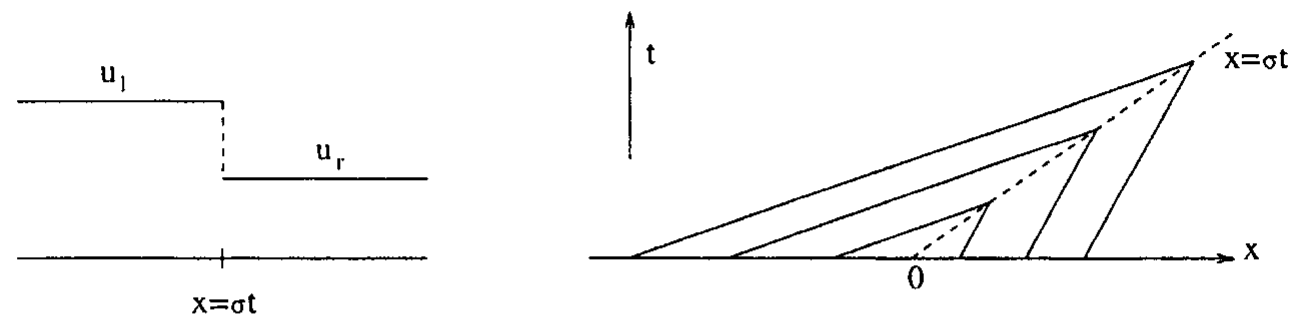
\includegraphics[width=.710\paperwidth]{images/fig-14-1-1.png}
  \caption{Riemann 问题的激波解(熵解)}\label{fig:14.1.1}
\end{figure}
\[
  \begin{aligned}
    0&=\frac{d}{dt}(u_l+u_r)
     =\frac{d}{dt}\biggl[\int_{\sigma t-1}^{\sigma t}u(t,x)\,\mathrm dx
                        +\int_{\sigma t}^{\sigma t+1}u(t,x)\,\mathrm dx\biggr]\\
     &=\int_{\sigma t-1}^{\sigma t+1}\frac{\partial u}{\partial t}(t,x)\,\mathrm dx
                      -\sigma(u_l-u_r),
  \end{aligned}
\]
从而
\begin{equation}\label{eq:14.1.30}
  \sigma(u_l-u_r)=F(u_l)-F(u_r).
\end{equation}
这个关系对任意通量函数 \(F\) 都成立.对于 Burgers 方程,\(F(u)=u^2/2\),故 \(\sigma\) 取\eqref{eq:14.1.28}的形式.

关系\eqref{eq:14.1.30}称为 \emph{Rankine--Hugoniot 跳跃条件}.在更一般的情形下,任一激波的两侧都满足这个条件.此时,\(u_l\) 和 \(u_r\) 分别表示解在间断处的左值和右值,\(\sigma\) 则是相应的瞬时速度.

当 \(u_l<u_r\) 时,有无穷多个弱解.其中一个仍是\eqref{eq:14.1.27},见\figref{fig:14.1.2},但此时特征线从间断向外发出.可以证明这个解不稳定：数据的微小扰动会导致解发生显著变化.
\begin{figure}[htbp]
  \centering
  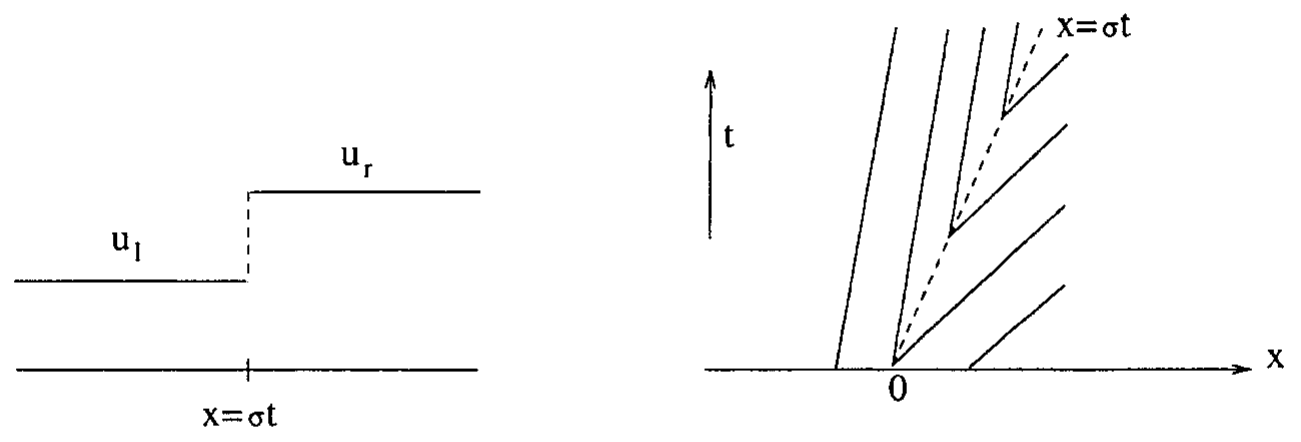
\includegraphics[width=.710\paperwidth]{images/fig-14-1-2.png}
  \caption{Riemann 问题中违反熵条件的解}\label{fig:14.1.2}
\end{figure}
另一个在扰动下稳定的弱解是
\SourcePage{467}
\begin{equation}\label{eq:14.1.31}
  u(t,x)=\begin{cases}
    u_l, & x<u_lt,\\
    x/t, & u_lt\le x\le u_rt,\\
    u_r, & x>u_rt.
  \end{cases}
\end{equation}
这就是 Burgers 方程的消失黏性解,也就是熵解,见\figref{fig:14.1.3}.
\end{example}

前面的讨论说明了如何构造熵条件.如上所见,时间向前推进时,激波两侧的特征线应当进入间断.如果特征线从间断向外发出,那么初始数据或方程本身的微小扰动,例如加入少量黏性,都可能使解发生很大变化,典型结果是形成特征线的稀疏扇.

因此可得如下判据.传播速度 \(\sigma\) 由\eqref{eq:14.1.30}给出的间断,在下列条件下满足熵条件：
\begin{equation}\label{eq:14.1.32}
  F'(u_l)>\sigma>F'(u_r).
\end{equation}
当 \(F\) 严格凸时,Rankine--Hugoniot 条件\eqref{eq:14.1.30}表明,\(\sigma\) 必介于 \(F'(u_l)\) 与 \(F'(u_r)\) 之间.所以\eqref{eq:14.1.32}只要求 \(F'(u_l)>F'(u_r)\),根据严格凸性,这等价于 \(u_l>u_r\).

当 \(F\) 非凸时,可采用下面更一般的判据.传播速度 \(\sigma\) 由\eqref{eq:14.1.30}给出的间断,若对所有介于 \(u_l\) 和 \(u_r\) 之间的 \(u\) 都有
\begin{equation}\label{eq:14.1.33}
  \frac{F(u)-F(u_l)}{u-u_l}\ge\sigma
       \ge\frac{F(u)-F(u_r)}{u-u_r},
\end{equation}
则满足熵条件.

熵条件的另一种表述使用熵函数与熵通量.从守恒律\eqref{eq:14.1.20}出发,假定对光滑解 \(u\),有一对函数 \(\eta(u)\) 和 \(\mu(u)\) 满足
\begin{equation}\label{eq:14.1.34}
  \frac{\partial}{\partial t}\eta(u)+\frac{\partial}{\partial x}\mu(u)=0.
\end{equation}
\begin{definition*}
函数 \(\eta(u)\) 和 \(\mu(u)\) 分别称为{\heiti 熵函数}和{\heiti 熵通量}.
\end{definition*}
函数 \(\eta\)、\(\mu\) 与 \(F\) 的关系为
\begin{equation}\label{eq:14.1.35}
  \mu'(u)=\eta'(u)F'(u).
\end{equation}
事实上,设 \(u\) 光滑,由\eqref{eq:14.1.34}有
\[
  \eta'(u)\frac{\partial u}{\partial t}
        +\mu'(u)\frac{\partial u}{\partial x}=0,
\]
而由\eqref{eq:14.1.20},
\SourcePage{468}
\begin{figure}[htbp]
  \centering
  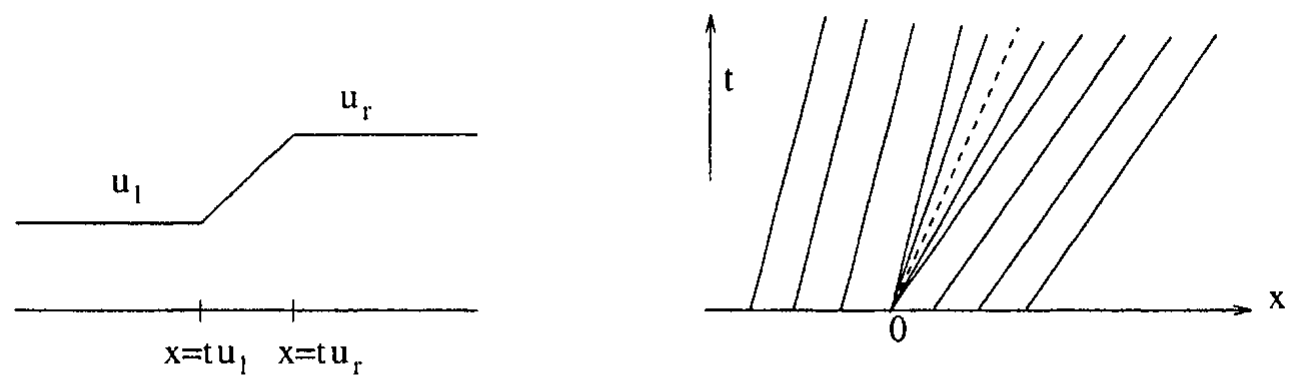
\includegraphics[width=.709\paperwidth]{images/fig-14-1-3.png}
  \caption{Riemann 问题的稀疏波解(熵解)}\label{fig:14.1.3}
\end{figure}
\[
  0=\eta'(u)\biggl[\frac{\partial u}{\partial t}
                      +F'(u)\frac{\partial u}{\partial x}\biggr].
\]
比较两式即得\eqref{eq:14.1.35}.

熵条件的第三种表述如下.
\begin{definition*}
如果对所有凸熵函数 \(\eta(\cdot)\) 及对应的熵通量 \(\mu(\cdot)\),熵不等式
\begin{equation}\label{eq:14.1.36}
  \frac{\partial}{\partial t}\eta(u)+\frac{\partial}{\partial x}\mu(u)\le0
\end{equation}
均在弱意义下成立,那么称弱解 \(u(t,x)\) 为\eqref{eq:14.1.20}的{\heiti 熵解}.
\end{definition*}

可以用下面的启发式推导解释这一条件.利用\eqref{eq:14.1.25}和\eqref{eq:14.1.35},得到
\[
  \begin{aligned}
    \frac{\partial}{\partial t}\eta(u^\varepsilon)
        +\frac{\partial}{\partial x}\mu(u^\varepsilon)
      &=\eta'(u^\varepsilon)\biggl[
            \frac{\partial u^\varepsilon}{\partial t}
              +F'(u^\varepsilon)\frac{\partial u^\varepsilon}{\partial x}\biggr]
       =\varepsilon\eta'(u^\varepsilon)\frac{\partial^2u^\varepsilon}{\partial x^2}\\
      &=\varepsilon\biggl[
          \frac{\partial}{\partial x}\biggl(\eta'(u^\varepsilon)
                  \frac{\partial u^\varepsilon}{\partial x}\biggr)
          -\eta''(u^\varepsilon)\biggl(\frac{\partial u^\varepsilon}{\partial x}\biggr)^2\biggr]\\
      &\le\varepsilon\frac{\partial}{\partial x}\biggl(
                      \eta'(u^\varepsilon)\frac{\partial u^\varepsilon}{\partial x}\biggr).
  \end{aligned}
\]
令 \(\varepsilon\to0\) 并取 \(u:=\lim_{\varepsilon\to0}u^\varepsilon\),形式上即得\eqref{eq:14.1.36}.

\eqref{eq:14.1.36}的弱形式是
\begin{equation}\label{eq:14.1.37}
  \begin{aligned}
    &-\int_0^\infty\!\!\int_{-\infty}^\infty
     \biggl[\eta(u(t,x))\frac{\partial\varphi}{\partial t}(t,x)
           +\mu(u(t,x))\frac{\partial\varphi}{\partial x}(t,x)\biggr]
                   \,\mathrm dx\,\mathrm dt\\
    &\qquad\le\int_{-\infty}^\infty\varphi(0,x)\eta(u(0,x))\,\mathrm dx,
  \end{aligned}
\end{equation}
其中 \(\varphi\) 可取 \(C_0^1([0,\infty)\times\mathbb R)\) 中的任一函数,只要对所有 \((t,x)\in[0,\infty)\times\mathbb R\) 有 \(\varphi(t,x)\ge0\).

对于 \(F(u)=u^2/2\) 的 Burgers 方程,例如取 \(\eta(u)=u^2\),由\eqref{eq:14.1.35}得 \(\mu'(u)=2u^2\),故可取 \(\mu(u)=2u^3/3\).熵不等式\eqref{eq:14.1.36}成为
\begin{equation}\label{eq:14.1.38}
  \frac{\partial}{\partial t}u^2+\frac{\partial}{\partial x}\biggl(\frac23u^3\biggr)\le0.
\end{equation}
\SourcePage{469}
对于光滑解,等号成立.当出现间断时,可以证明\eqref{eq:14.1.38}成立当且仅当 \((u_l-u_r)^3>0\),即如所预期的 \(u_l>u_r\).对于给定的数值方法,可以用\eqref{eq:14.1.36}的离散形式检验数值解是否收敛到熵解.

综上,物理解 \(u=\lim_{\varepsilon\to0}u^\varepsilon\) 是\eqref{eq:14.1.20}的一类弱解,满足熵条件\eqref{eq:14.1.36}.\BookCite{kruzkov1970}{Kruzkov(1970)}证明,熵解存在,并由初始数据 \(u_0(x)\) 唯一确定.

关于非线性守恒律的深入分析,可参阅\BookCite{courant-friedrichs1948}{Courant 和 Friedrichs(1948)}、\BookCite{oleinik1957}{Oleinik(1957)}、\BookCite{lax1973}{Lax(1973)}和\BookCite{smoller1983}{Smoller(1983)}等.

\section{有限差分逼近}\label{sec:14.2}

为作基于有限差分的时空逼近,选取时间步长 \(\Delta t\) 和网格宽度 \(\Delta x\),以网格点 \((t_n,x_j)\) 离散 \((t,x)\) 平面,其中
\[
  t_n:=n\Delta t,\quad n=0,1,\ldots,\qquad
  x_j:=j\Delta x,\quad j\in\mathbb Z.
\]
定义网格比 \(\lambda:=\Delta t/\Delta x\),并记 \(x_{j+1/2}:=x_j+\Delta x/2\).我们要寻找对所有 \(j,n\) 逼近 \(u(t_n,x_j)\) 的离散解 \(u_j^n\).有时 \(u_j^n\) 用来逼近所谓的\emph{单元平均值}
\[
  \overline u_j^n:=\frac1{\Delta x}
    \int_{x_{j-1/2}}^{x_{j+1/2}}u(t_n,x)\,\mathrm dx.
\]
有限体积法经常采用后一种做法.

\subsection{线性标量对流方程与双曲型方程组}\label{sec:14.2.1}

双曲型初值问题一般用显式方法作时间推进,因而通常要限制网格比 \(\lambda\) 才能保持稳定性.隐式方法一般没有这一限制.\tabref{tab:14.2.1}列出了对 \(a\) 为常数的线性对流方程\eqref{eq:14.1.1}的几种格式.除蛙跳格式外,表中的方法都是两层格式,只涉及时间层 \(t_n\) 和 \(t_{n+1}\).

有些方法采用中心有限差分,即在逼近节点 \(x_j\) 处的 \(x\) 导数时,同时使用 \(u_{j-1}\) 和 \(u_{j+1}\).\emph{中心向前 Euler 法}是其中最简单的一个例子,见\tabref{tab:14.2.1}.可惜它不稳定,稳定性的定义见下一小节.Lax--Friedrichs 法是 Euler 法的一个小改动,仅把 \(u_j^n\) 换成 \(u_{j+1}^n\) 和
\SourcePage{470}
\(u_{j-1}^n\) 的平均值,从而获得更好的稳定性,见第~\BookRef{sec:14.2.2}{14.2.2}~节.另一些方法采用单边有限差分,迎风法和 Warming--Beam 法就属于这一类.

\begin{table}[htbp]
  \centering
  \caption{问题\eqref{eq:14.1.1}的显式有限差分格式}\label{tab:14.2.1}
  \small
  \setlength{\tabcolsep}{4pt}
  \renewcommand{\arraystretch}{1.45}
  \begin{tabular}{@{}lll@{}}
    \toprule
    格式 & 差分方程 & \shortstack[l]{数值通量函数\\\(h_{j+1/2}\)}\\
    \midrule
    \shortstack[l]{中心向前\\Euler}
      & \(u_j^{n+1}=u_j^n-\tfrac{\lambda}{2}a(u_{j+1}^n-u_{j-1}^n)\)
      & \(\tfrac12a(u_{j+1}+u_j)\)\\
    迎风
      & \(\begin{aligned}[t]
          u_j^{n+1}&=u_j^n-\tfrac{\lambda}{2}a(u_{j+1}^n-u_{j-1}^n)\\
            &\quad+\tfrac{\lambda}{2}|a|(u_{j+1}^n-2u_j^n+u_{j-1}^n)
         \end{aligned}\)
      & \(\begin{aligned}[t]
          &\tfrac12[a(u_{j+1}+u_j)\\
          &\qquad-|a|(u_{j+1}-u_j)]
        \end{aligned}\)\\
    \shortstack[l]{Lax--\\Friedrichs}
      & \(\begin{aligned}[t]
          u_j^{n+1}&=\tfrac12(u_{j+1}^n+u_{j-1}^n)\\
            &\quad-\tfrac{\lambda}{2}a(u_{j+1}^n-u_{j-1}^n)
         \end{aligned}\)
      & \(\begin{aligned}[t]
          &\tfrac12[a(u_{j+1}+u_j)\\
          &\qquad-\tfrac1\lambda(u_{j+1}-u_j)]
        \end{aligned}\)\\
    \shortstack[l]{Lax--\\Wendroff}
      & \(\begin{aligned}[t]
          u_j^{n+1}&=u_j^n-\tfrac{\lambda}{2}a(u_{j+1}^n-u_{j-1}^n)\\
            &\quad+\tfrac{\lambda^2}{2}a^2(u_{j+1}^n-2u_j^n+u_{j-1}^n)
         \end{aligned}\)
      & \(\begin{aligned}[t]
          &\tfrac12[a(u_{j+1}+u_j)\\
          &\qquad-\lambda a^2(u_{j+1}-u_j)]
        \end{aligned}\)\\
    \shortstack[l]{Warming--\\Beam (\(a>0\))}
      & \(\begin{aligned}[t]
          u_j^{n+1}&=u_j^n-\tfrac{\lambda}{2}a(3u_j^n-4u_{j-1}^n+u_{j-2}^n)\\
            &\quad+\tfrac{\lambda^2}{2}a^2(u_j^n-2u_{j-1}^n+u_{j-2}^n)
         \end{aligned}\)
      & \(\begin{aligned}[t]
          &\tfrac12[a(3u_j-u_{j-1})\\
          &\qquad-\lambda a^2(u_j-u_{j-1})]
        \end{aligned}\)\\
    蛙跳 & \(u_j^{n+1}=u_j^{n-1}-\lambda a(u_{j+1}^n-u_{j-1}^n)\) & \\
    \bottomrule
  \end{tabular}
\end{table}

\emph{迎风法}的推导如下.
\SourcePage{471}
\begin{equation}\label{eq:14.2.1}
  \frac{u_j^{n+1}-u_j^n}{\Delta t}
    =\begin{cases}
       -\dfrac{a}{\Delta x}(u_{j+1}^n-u_j^n), & a<0,\\[4pt]
       -\dfrac{a}{\Delta x}(u_j^n-u_{j-1}^n), & a>0.
     \end{cases}
\end{equation}
等价地,可写为
\begin{equation}\label{eq:14.2.2}
  \frac{u_j^{n+1}-u_j^n}{\Delta t}
    +a\frac{u_{j+1}^n-u_{j-1}^n}{2\Delta x}
    =\tfrac12|a|\Delta x
         \frac{u_{j+1}^n-2u_j^n+u_{j-1}^n}{(\Delta x)^2}.
\end{equation}
与中心向前 Euler 法相比,\eqref{eq:14.2.2}的右端增加了一项
\begin{equation}\label{eq:14.2.3}
  \varepsilon\frac{u_{j+1}^n-2u_j^n+u_{j-1}^n}{(\Delta x)^2},
\end{equation}
其中 \(\varepsilon=\tfrac12|a|\Delta x\).因为 \((u_{j+1}-2u_j+u_{j-1})/(\Delta x)^2\) 是 \(x_j\) 处 \(\partial^2u/\partial x^2\) 的一个逼近,\eqref{eq:14.2.3}就是为稳定格式而加入的\emph{人工黏性}项,也称\emph{数值耗散}项.

\emph{Lax--Wendroff 法}从关于 \(t=t_n\) 的二阶 Taylor 展开出发,而无须直接对\eqref{eq:14.1.1}中的时空导数作有限差分逼近：
\[
  \begin{aligned}
    u(t_{n+1},x_j)
      &=u(t_n,x_j)+\Delta t\frac{\partial u}{\partial t}(t_n,x_j)\\
      &\qquad+\tfrac12(\Delta t)^2\frac{\partial^2u}{\partial t^2}(t_n,x_j)
                +O((\Delta t)^3).
  \end{aligned}
\]
利用\eqref{eq:14.1.1}可得
\[
  \frac{\partial u}{\partial t}=-a\frac{\partial u}{\partial x},
  \qquad \frac{\partial^2u}{\partial t^2}=a^2\frac{\partial^2u}{\partial x^2}.
\]
将这两式代入,保留 Taylor 展开右端的前三项,再用中心有限差分逼近空间导数,就得到 Lax--Wendroff 法.

\emph{Warming--Beam 法}的推导类似,不过空间导数采用单边差分逼近.\tabref{tab:14.2.1}给出的是 \(a>0\) 时的公式.

容易看出,Lax--Friedrichs 法引入的数值耗散仍具有\eqref{eq:14.2.3}的形式,其中 \(\varepsilon=(\Delta x)^2/(2\Delta t)\).Lax--Wendroff 法中对应的系数为 \(\varepsilon=\tfrac12a^2\Delta t\).

分别在模板 \((j-1,j,j+1)\) 和 \((j-2,j-1,j)\) 上,Lax--Wendroff 格式和 Warming--Beam 格式是唯一具有二阶精度的两层格式.参见\BookCite{hirsch1988}{Hirsch(1988,第 357–360 页)}.若把它们视为下列修正\emph{色散}方程的直接逼近,两种方法实际上都具有三阶精度：
\[
  \frac{\partial u}{\partial t}+a\frac{\partial u}{\partial x}
    =\varepsilon\frac{\partial^3u}{\partial x^3}.
\]
\SourcePage{472}
具体而言,Lax--Wendroff 格式的色散系数为 \(\varepsilon=\tfrac{(\Delta x)^2}{6}a(\lambda^2a^2-1)\),Warming--Beam 格式的为 \(\varepsilon=\tfrac{(\Delta x)^2}{6}a(2-3\lambda a+\lambda^2a^2)\).关于色散波理论,\BookCite{whitham1974}{Whitham(1974)}有详尽论述.

\tabref{tab:14.2.1}中的两层显式有限差分法都可写成统一形式
\begin{equation}\label{eq:14.2.4}
  u_j^{n+1}=u_j^n-\lambda(h_{j+1/2}^n-h_{j-1/2}^n),
\end{equation}
其中通常取 \(h_{j+1/2}=h(u_j,u_{j+1})\),Warming--Beam 法在 \(a>0\) 时则取 \(h_{j+1/2}=h(u_{j-1},u_j)\).函数 \(h(\cdot,\cdot)\) 称为\emph{数值通量函数},各方法的具体表达式见\tabref{tab:14.2.1}.

简洁形式\eqref{eq:14.2.4}的优点是便于推广到更一般的双曲型问题,尤其是线性方程组和非线性方程.考虑方程组\eqref{eq:14.1.6}时,仍可按\tabref{tab:14.2.1}作有限差分逼近,只须留意记号的变化.首先,把 \(a\) 换成矩阵 \(A\),把 \(a^2\) 换成 \(A^2\),并以逼近 \(\boldsymbol{U}(t_n,x_j)\) 的向量 \(\boldsymbol{U}_j^n\) 代替 \(u_j^n\).此外,在迎风法中,应以
\begin{equation}\label{eq:14.2.5}
  |A|:=T|\Lambda|T^{-1}
\end{equation}
代替 \(|a|\),其中 \(|\Lambda|:=\operatorname{diag}(|\lambda_1|,\ldots,|\lambda_p|)\),见\eqref{eq:14.1.7}.

这一公式的来由很容易理解.先将方程组\eqref{eq:14.1.6}变换为 \(p\) 个独立的对流方程\eqref{eq:14.1.9},再对其中每个方程应用标量迎风格式.这样得到
\[
  \begin{aligned}
    (W_k)_j^{n+1}&=(W_k)_j^n-\tfrac{\lambda}{2}\lambda_k
                       [(W_k)_{j+1}^n-(W_k)_{j-1}^n]\\
        &\qquad+\tfrac{\lambda}{2}|\lambda_k|
                  [(W_k)_{j+1}^n-2(W_k)_j^n+(W_k)_{j-1}^n],
  \end{aligned}
\]
其中 \(k=1,\ldots,p\).用紧凑记号写为
\[
  \boldsymbol{W}_j^{n+1}=\boldsymbol{W}_j^n-\tfrac{\lambda}{2}\Lambda(\boldsymbol{W}_{j+1}^n-\boldsymbol{W}_{j-1}^n)
     +\tfrac{\lambda}{2}|\Lambda|(\boldsymbol{W}_{j+1}^n-2\boldsymbol{W}_j^n+\boldsymbol{W}_{j-1}^n).
\]
通过变换 \(T\boldsymbol{W}_j^n=\boldsymbol{U}_j^n\) 回到物理变量 \(\boldsymbol{U}_j^n\),便得到向量迎风法
\begin{equation}\label{eq:14.2.6}
  \begin{aligned}
    \boldsymbol{U}_j^{n+1}
      &=\boldsymbol{U}_j^n-\tfrac{\lambda}{2}A(\boldsymbol{U}_{j+1}^n-\boldsymbol{U}_{j-1}^n)\\
      &\qquad+\tfrac{\lambda}{2}|A|(\boldsymbol{U}_{j+1}^n-2\boldsymbol{U}_j^n+\boldsymbol{U}_{j-1}^n).
  \end{aligned}
\end{equation}
向量情形下,上述两层时间推进格式也可改写为
\begin{equation}\label{eq:14.2.7}
  \boldsymbol{U}_j^{n+1}=\boldsymbol{U}_j^n
       -\lambda(\boldsymbol{H}_{j+1/2}^n-\boldsymbol{H}_{j-1/2}^n),
\end{equation}
\SourcePage{473}
其中 \(\boldsymbol{H}_{j+1/2}\) 为\emph{数值通量向量函数}.它的表达式很容易由标量情形推广得到,即分别用 \(A\)、\(A^2\)、\(|A|\) 代替 \(a\)、\(a^2\)、\(|a|\).

\subsection{稳定性、相容性与收敛性}\label{sec:14.2.2}

任意两层方法都可写成紧凑形式
\begin{equation}\label{eq:14.2.8}
  \boldsymbol{u}^{n+1}=E_{\Delta t}(\boldsymbol{u}^n),
\end{equation}
其中 \(\boldsymbol{u}^n\) 表示 \(t_n\) 时刻的近似值向量 \(\{u_j^n\mid j\in\mathbb Z\}\).按分量写为
\begin{equation}\label{eq:14.2.9}
  u_j^{n+1}=E_{\Delta t}(\boldsymbol{u}^n;j).
\end{equation}
例如,中心向前 Euler 法的算子 \(E_{\Delta t}\) 取形式
\begin{equation}\label{eq:14.2.10}
  E_{\Delta t}(\boldsymbol{u}^n;j)=u_j^n-\tfrac{\lambda a}{2}(u_{j+1}^n-u_{j-1}^n).
\end{equation}

\begin{definition*}
如果对任意 \(T>0\),均存在常数 \(C_T>0\)(可依赖于 \(T\))和 \(\delta_0>0\),使得对所有满足 \(n\Delta t\le T\)、\(0<\Delta t\le\delta_0\)、\(0<\Delta x\le\delta_0\) 的允许网格和时间层,都有
\begin{equation}\label{eq:14.2.11}
  \|\boldsymbol{u}^n\|_\Delta\le C_T\|\boldsymbol{u}^0\|_\Delta,
\end{equation}
则称该方法在 Lax--Richtmyer 意义下{\heiti 稳定}.这里
\begin{equation}\label{eq:14.2.12}
  \|\boldsymbol{v}\|_\Delta:=\Delta x\sum_{j=-\infty}^{\infty}|v_j|
\end{equation}
是 \(L^1(\mathbb R)\) 范数的离散近似,见\eqref{eq:14.1.5}.
\end{definition*}
由于 \(\boldsymbol{u}^n=E_{\Delta t}^n(\boldsymbol{u}^0)\),只要存在 \(\beta\ge0\),使得对每个允许的 \(0<\Delta t\le\delta_0\)、\(0<\Delta x\le\delta_0\),都有
\[
  \|E_{\Delta t}\boldsymbol{v}\|_\Delta
      \le(1+\beta\Delta t)\|\boldsymbol{v}\|_\Delta\qquad\forall\boldsymbol{v},
\]
稳定性便成立.事实上,当 \(n\Delta t\le T\) 时,
\[
  \|\boldsymbol{u}^n\|_\Delta\le(1+\beta\Delta t)^n\|\boldsymbol{u}^0\|_\Delta
       \le e^{\beta T}\|\boldsymbol{u}^0\|_\Delta,
\]
从而得到\eqref{eq:14.2.11}.

现在讨论相容性.定义\emph{局部截断误差}为
\[
  (\mathcal T_{\Delta t}(t))_j
     :=\frac1{\Delta t}[u(t+\Delta t,x_j)-E_{\Delta t}(u(t);j)],
\]
其中 \(E_{\Delta t}(u(t);j)\) 随所用的两层方法而定,其定义是在\eqref{eq:14.2.9}右端用 \(u(t,x_j)\) 代替 \(u_j^n\).
\SourcePage{474}
\begin{definition*}
若沿所选网格族,随着 \(\Delta t,\Delta x\to0\),对所有 \(t>0\) 都有
\begin{equation}\label{eq:14.2.13}
  \lim_{\Delta t,\Delta x\to0}\|\mathcal T_{\Delta t}(t)\|_\Delta=0,
\end{equation}
则称两层方法{\heiti 相容}.进一步,如果对所有足够光滑的初始数据,都有某个常数 \(C>0\),使得
\begin{equation}\label{eq:14.2.14}
  \|\mathcal T_{\Delta t}(t)\|_\Delta\le C[(\Delta t)^{q_1}+(\Delta x)^{q_2}],
    \qquad t>0
\end{equation}
对所有允许的 \(0<\Delta t\le\delta_0\)、\(0<\Delta x\le\delta_0\) 成立,就称该方法在时间上为 \(q_1\) 阶,在空间上为 \(q_2\) 阶.
\end{definition*}
离散时,\(\Delta t\) 和 \(\Delta x\) 常成正比,即对某个正常数 \(\kappa\) 有 \(\Delta t=\kappa\Delta x\).此时称方法为 \(q\) 阶,其中 \(q=\min(q_1,q_2)\).还应指出,当用方法\eqref{eq:14.2.8}逼近定常解时,起决定作用的是空间阶,也就是 \(\Delta x\) 的指数 \(q_2\).

\begin{definition*}
如果当 \(\Delta t,\Delta x\to0\) 时有
\[
  \max_{0\le n\le T/\Delta t}\|u(t_n,\cdot)-\boldsymbol{u}^n\|_\Delta\to0,
\]
则称该格式{\heiti 收敛}.
\end{definition*}

线性双曲型初值问题理论的基本结果是 Lax--Richtmyer 等价定理.
\begin{theorem*}
对适定的线性初值问题,相容的线性差分方法收敛的充要条件是稳定性.
\end{theorem*}
Lax--Richtmyer 等价定理的证明见\BookCite{richtmyer-morton1967}{Richtmyer 和 Morton(1967)},另见\BookCite{strikwerda1989}{Strikwerda(1989)}.

下面说明几个稳定性结果.例如,对 Lax--Friedrichs 法,有
\[
  \|\boldsymbol{u}^{n+1}\|_\Delta=\Delta x\sum_j|u_j^{n+1}|
     \le\frac{\Delta x}{2}
       \biggl[\sum_j|(1-\lambda a)u_{j+1}^n|
                     +\sum_j|(1+\lambda a)u_{j-1}^n|\biggr].
\]
假定
\begin{equation}\label{eq:14.2.15}
  |a\lambda|=\biggl|a\frac{\Delta t}{\Delta x}\biggr|\le1,
\end{equation}
则 \(1-\lambda a\) 和 \(1+\lambda a\) 都非负,因而
\[
  \begin{aligned}
    \|\boldsymbol{u}^{n+1}\|_\Delta
       &\le\frac{\Delta x}{2}\biggl[(1-a\lambda)\sum_j|u_{j+1}^n|
                        +(1+a\lambda)\sum_j|u_{j-1}^n|\biggr]\\
       &\le\tfrac12(1-a\lambda)\|\boldsymbol{u}^n\|_\Delta
             +\tfrac12(1+a\lambda)\|\boldsymbol{u}^n\|_\Delta=\|\boldsymbol{u}^n\|_\Delta.
  \end{aligned}
\]
因此,只要满足稳定性限制\eqref{eq:14.2.15},\eqref{eq:14.2.11}便以 \(C_T=1\) 成立.

类似地,只要 \(\Delta t\) 和 \(\Delta x\) 满足\eqref{eq:14.2.15},就可证明迎风法稳定.事实上,当 \(a>0\) 时,迎风格式\eqref{eq:14.2.1}为
\SourcePage{475}
\[
  u_j^{n+1}=u_j^n-\lambda a(u_j^n-u_{j-1}^n).
\]
于是
\[
  \|\boldsymbol{u}^{n+1}\|_\Delta\le\Delta x\sum_j|(1-\lambda a)u_j^n|
                            +\Delta x\sum_j|\lambda a u_{j-1}^n|.
\]
若\eqref{eq:14.2.15}成立,则 \(u_j^n\) 和 \(u_{j-1}^n\) 的系数均非负,故 \(\|\boldsymbol{u}^{n+1}\|_\Delta\le\|\boldsymbol{u}^n\|_\Delta\).\(a<0\) 时也得到同样的结果.

中心向前 Euler 法在类似\eqref{eq:14.2.15}的限制下会失稳.不过,在离散 \(L^2\) 范数下,取 \(\Delta t=O((\Delta x)^2)\) 可使它稳定.参见\BookCite{strikwerda1989}{Strikwerda(1989,第 49 页)}.

将\eqref{eq:14.2.15}中的不等号改为严格不等号,并使 \(|\lambda a|\) 一致小于 \(1\),也足以保证蛙跳格式在离散 \(L^2\) 范数下稳定.事实上,用 \(u_j^{n+1}+u_j^{n-1}\) 乘蛙跳方程并求和,得
\[
  \begin{aligned}
    &\sum_j[(u_j^{n+1})^2+\lambda a(u_j^{n+1}u_{j+1}^n-u_{j-1}^n u_j^{n+1})]\\
    &\quad=\sum_j[(u_j^{n-1})^2+\lambda a(u_{j-1}^n u_j^{n-1}-u_j^{n-1}u_{j+1}^n)].
  \end{aligned}
\]
在两端各加上 \(\sum_j(u_j^n)^2\),并注意对每个 \(k\ge0\),由移项求和有
\[
  \sum_i u_{i-1}^k u_i^{k+1}
    =\sum_i\bigl[u_i^k u_{i+1}^{k+1}
        -(u_i^k u_{i+1}^{k+1}-u_{i-1}^k u_i^{k+1})\bigr]
    =\sum_i u_i^k u_{i+1}^{k+1},
\]
就可从上一等式得到
\[
  \sum_j G_j^{n+1}=\sum_j G_j^n,
\]
其中
\[
  G_j^n:=(u_j^n)^2+(u_j^{n-1})^2
          +a\lambda(u_j^n u_{j+1}^{n-1}-u_{j+1}^n u_j^{n-1}).
\]
因此,\(\sum_j G_j^{n+1}=\sum_j G_j^1\),即
\[
  \begin{aligned}
    &\sum_j[(u_j^{n+1})^2+(u_j^n)^2+\lambda a(u_j^{n+1}u_{j+1}^n-u_{j+1}^{n+1}u_j^n)]\\
    &\quad=\sum_j[(u_j^1)^2+(u_j^0)^2+\lambda a(u_j^1u_{j+1}^0-u_{j+1}^1u_j^0)].
  \end{aligned}
\]
利用不等式 \(-x^2-y^2\le2xy\le x^2+y^2\),可得
\[
  (1-|\lambda a|)\sum_j[(u_j^{n+1})^2+(u_j^n)^2]
     \le(1+|\lambda a|)\sum_j[(u_j^1)^2+(u_j^0)^2].
\]
设 \(|\lambda a|\le c<1\),其中 \(c\) 固定.因此,对每个 \(T\),存在常数 \(C_T>0\),使得所有满足 \(n\Delta t\le T\) 的 \(n\) 均有
\SourcePage{476}
\[
  \|\boldsymbol{u}^n\|_{2,\Delta}
    \le C_T(\|\boldsymbol{u}^0\|_{2,\Delta}^2+\|\boldsymbol{u}^1\|_{2,\Delta}^2)^{1/2},
  \qquad
  \|\boldsymbol{v}\|_{2,\Delta}:=\biggl(\Delta x\sum_j|v_j|^2\biggr)^{1/2}.
\]
这一稳定性不等式在离散 \(L^2\) 范数下将\eqref{eq:14.2.11}推广到三层有限差分格式.

用类似方法可以证明,Lax--Wendroff 法在相同的限制\eqref{eq:14.2.15}下也是稳定的,范数仍取离散 \(L^2\) 范数.

另一种证明稳定性的方法是 von Neumann 分析,它对有限差分方程作 Fourier 变换.这种方法在\BookCite{richtmyer-morton1967}{Richtmyer 和 Morton(1967)}和\BookCite{strikwerda1989}{Strikwerda(1989)}中有详尽讨论,另见\BookCite{vichnevetsky-bowles1982}{Vichnevetsky 和 Bowles(1982)}.Warming--Beam 格式的一个基于 von Neumann 分析的稳定性证明,见\BookCite{hirsch1988}{Hirsch(1988,第 9.3 节)}.其稳定性条件是 \(|a\lambda|\le2\),对 \(\lambda\) 的限制比\eqref{eq:14.2.15}宽松.原因在于,\emph{差分模板}是把计算 \(u_j^{n+1}\) 涉及的所有网格点连接起来的图.Warming--Beam 格式的模板在 \(x_j\) 的一侧用了两个点.

更确切地说,稳定性条件可作如下几何解释.对于具有 Lax--Wendroff 型模板的有限差分格式,\(u_j^{n+1}\) 依赖于上一时间层在 \(x_{j+i}\)(\(i=-1,0,1\))三个点的值.一直回溯到 \(t=0\),可见 \(u_j^{n+1}\) 只依赖于 \(i=-(n+1),\ldots,n+1\) 对应的 \(x_{j+i}\) 处的初始数据.因此,\(u_j^n\) 的\emph{数值依赖域} \(D_{\Delta t}(t_n,x_j)\) 满足
\[
  D_{\Delta t}(t_n,x_j)\subset
    \bigl\{x\in\mathbb R\mid |x-x_j|\le n\Delta x=t_n/\lambda\bigr\}.
\]
对任一固定点 \((\bar t,\bar x)\),相应地有
\[
  D_{\Delta t}(\bar t,\bar x)\subset
    \bigl\{x\in\mathbb R\mid |x-\bar x|\le\bar t/\lambda\bigr\}.
\]
特别地,保持 \(\lambda\) 固定并令 \(\Delta t\to0\),极限数值依赖域为
\[
  D_0(\bar t,\bar x)=\bigl\{x\in\mathbb R\mid |x-\bar x|\le\bar t/\lambda\bigr\}.
\]
条件\eqref{eq:14.2.15}等价于
\begin{equation}\label{eq:14.2.16}
  D(\bar t,\bar x)\subset D_0(\bar t,\bar x),
\end{equation}
其中 \(D(\bar t,\bar x)\) 是\eqref{eq:14.1.11}定义的依赖域.由于现在考虑标量情形,这里 \(p=1\)、\(\lambda_1=a\).

对于一致格式,这个条件是稳定性的必要条件.事实上,若不满足它,精确依赖域中就存在某个点 \(y^*\),
\SourcePage{477}
不属于数值依赖域.改变 \(y^*\) 附近的初始数据会改变精确解,却不会改变数值解,因而无法收敛.根据 Lax--Richtmyer 等价定理,这也排除了稳定性.

\begin{definition*}
\eqref{eq:14.2.15}称为 {\heiti CFL 条件}.\BookCite{courant-friedrichs-lewy1928}{Courant、Friedrichs 和 Lewy(1928)}证明,这是数值解稳定的一个必要条件.特别地,对双曲型初值问题,任何采用固定有限模板的显式相容有限差分格式都要受这一类稳定性限制.
\end{definition*}
在上面的一些例子中,CFL 条件既是数值格式稳定的必要条件,也是充分条件.不过,也有方法在满足 CFL 条件时仍不稳定.

向量情形也有类似的稳定性条件.例如,将 Lax--Wendroff 型模板用于\eqref{eq:14.1.6}时,步长须满足
\begin{equation}\label{eq:14.2.17}
  \biggl|\lambda_k\frac{\Delta t}{\Delta x}\biggr|\le1,\qquad k=1,\ldots,p,
\end{equation}
其中 \(\{\lambda_k\mid k=1,\ldots,p\}\) 是 \(A\) 的特征值.这些条件也可写成\eqref{eq:14.2.16}的形式.换言之,每条直线 \(x=\bar x-\lambda_k(\bar t-t)\) 与时间层 \(t=\bar t-\Delta t\) 的交点 \(x^{(k)}\) 都必须落在差分模板的底边上,见\figref{fig:14.2.1}.

\begin{figure}[htbp]
  \centering
  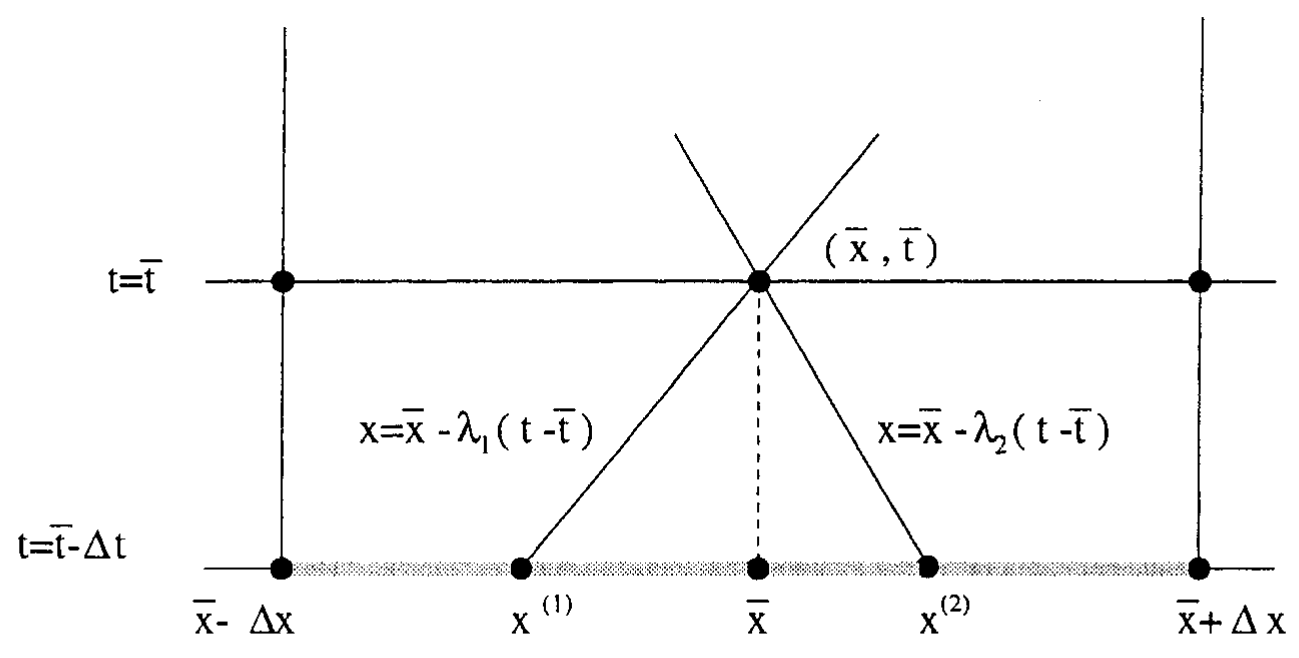
\includegraphics[width=.709\paperwidth]{images/fig-14-2-1.png}
  \caption{CFL 条件\eqref{eq:14.2.17}的几何解释}\label{fig:14.2.1}
\end{figure}

\begin{note}
\NumberedNote{note:14.2.1}{\heiti(边界处理)}考虑 \(a>0\) 时的下列初边值问题：
\SourcePage{478}
\[
  \begin{cases}
    \dfrac{\partial u}{\partial t}+a\dfrac{\partial u}{\partial x}=0,
        & t>0,\quad 0<x<1,\\[2pt]
    u(t,0)=\varphi_-(t), & t>0,\\
    u(0,x)=u_0(x), & 0<x<1.
  \end{cases}
\]
选定正整数 \(M\) 后,令 \(\Delta x:=1/M\),\(x_j:=j\Delta x\),\(j=0,\ldots,M\).

有限差分格式在每个内部点 \(x_j\)(\(j=1,\ldots,M-1\))离散微分方程,并在流入点施加给定的边界条件.许多有限差分格式还须添加边界条件才能唯一确定数值解,这些附加条件通常称为{\heiti 数值边界条件}.例如,采用 Lax--Wendroff 法或 Lax--Friedrichs 法时,格式无法直接用于流出点 \(x_M\),因为它需要计算区间 \([0,1]\) 外的 \(x_{M+1}\) 处的 \(u_{M+1}^n\).一般用外推公式求出 \(u_M^{n+1}\),外推可有多种形式.例如,可取 \(u_M^{n+1}=u_{M-1}^{n+1}\)(常值外推),或取 \(u_M^{n+1}=2u_{M-1}^{n+1}-u_{M-2}^{n+1}\)(线性外推),还可取 \(u_M^{n+1}=2u_{M-1}^n-u_{M-2}^{n-1}\)(沿特征线的近似线性外推).

还可用单边差分格式导出数值边界条件.例如,对 Lax--Wendroff 法,可以用
\[
  u_M^{n+1}=u_M^n-\lambda a(u_M^n-u_{M-1}^n).
\]
这是在流出点 \((t_{n+1},x_M)\) 应用 Lax--Wendroff 格式,并用线性外推公式 \(u_{M+1}^n=2u_M^n-u_{M-1}^n\) 计算 \(u_{M+1}^n\) 得到的.

需要强调,数值边界条件有时会使原本对纯初值问题稳定的有限差分格式失稳.例如,对蛙跳格式,常值外推和线性外推均不稳定,沿特征线外推则稳定.对隐式 Crank--Nicolson 格式,上述结论正好相反.

关于数值边界条件的详尽分析,见\BookCite{strikwerda1989}{Strikwerda(1989,第 11 章)}.\hfill\(\square\)
\end{note}

\subsection{非线性标量方程}\label{sec:14.2.3}
\SourcePage{479}

考虑非线性标量守恒律
\begin{equation}\label{eq:14.2.18}
  \begin{cases}
    \dfrac{\partial u}{\partial t}+\dfrac{\partial}{\partial x}F(u)=0,
       &t>0,\quad x\in\mathbb R,\\[2pt]
    u(0,x)=u_0(x), &x\in\mathbb R,
  \end{cases}
\end{equation}
并以 \(a(u):=F'(u)\) 表示特征速度.

这里着重考虑间断解.对于光滑解,第~\ref{sec:14.2}~节已介绍的方法通常可以有效地用于线性化方程.不过,从第~\ref{sec:14.1.4}~节已经知道,即使初始数据光滑,也很容易产生间断解.间断解的数值逼近很有挑战性,至今仍是一个活跃的研究领域.本小节只介绍几个基本概念,并举例说明一些激波捕捉格式.系统介绍可参阅\BookCite{yee1989}{Yee(1989)}、\BookCite{leveque1990}{LeVeque(1990)}、\BookCite{godlewski-raviart1991}{Godlewski 和 Raviart(1991)}及其中的参考文献.

与线性情形一样,\emph{守恒形式}的三点显式有限差分格式一般按如下原则构造：
\begin{equation}\label{eq:14.2.19}
  u_j^{n+1}=u_j^n-\lambda(h_{j+1/2}^n-h_{j-1/2}^n),
\end{equation}
其中仍有 \(h_{j+1/2}^n:=h(u_j^n,u_{j+1}^n)\),\(h(\cdot,\cdot)\) 为\emph{数值通量函数}.最一般的情形可写成
\[
  u_j^{n+1}=u_j^n-\lambda[H(u_{j-p}^n,\ldots,u_{j+q}^n)
                              -H(u_{j-p-1}^n,\ldots,u_{j+q-1}^n)],
\]
其中 \(H\) 是一个有 \(p+q+1\) 个变量的函数,\(p,q\ge0\).

下面用一个推导说明\eqref{eq:14.2.19}的由来.由\eqref{eq:14.2.18}得
\[
  \begin{aligned}
    \int_{x_{j-1/2}}^{x_{j+1/2}}u(t_{n+1},x)\,\mathrm dx
      &=\int_{x_{j-1/2}}^{x_{j+1/2}}u(t_n,x)\,\mathrm dx\\
      &\quad-\biggl[\int_{t_n}^{t_{n+1}}F(u(t,x_{j+1/2}))\,\mathrm dt
                -\int_{t_n}^{t_{n+1}}F(u(t,x_{j-1/2}))\,\mathrm dt\biggr].
  \end{aligned}
\]
两端除以 \(\Delta x\),并用本节开头定义的单元平均值 \(\overline u_j^n\),得到
\[
  \overline u_j^{n+1}=\overline u_j^n
    -\frac1{\Delta x}\biggl[\int_{t_n}^{t_{n+1}}F(u(t,x_{j+1/2}))\,\mathrm dt
                   -\int_{t_n}^{t_{n+1}}F(u(t,x_{j-1/2}))\,\mathrm dt\biggr].
\]
与\eqref{eq:14.2.19}比较可知
\[
  h_{j+1/2}^n\simeq\frac1{\Delta t}\int_{t_n}^{t_{n+1}}
                    F(u(t,x_{j+1/2}))\,\mathrm dt,
\]
\SourcePage{480}
即数值通量函数相当于时间区间 \([t_n,t_{n+1}]\) 内通过 \(x_{j+1/2}\) 的平均通量.

为与守恒律\emph{相容},要求数值通量函数在常值解情形下化为真实通量 \(F\),即
\begin{equation}\label{eq:14.2.20}
  h(\overline u_0,\overline u_0)=F(\overline u_0),
     \qquad u(t,x)\equiv\overline u_0.
\end{equation}
此外,还要求 \(h\) 对每个变量都是 Lipschitz 连续的.

如第~\ref{sec:14.2.2}~节所见,线性问题的稳定性分析已经相当成熟.然而,线性化方程的局部稳定性对于非线性问题的稳定性既非必要条件,也非充分条件,尤其是在有强间断时.数值方法可能对线性化问题稳定,却在非线性问题上失稳,这称为\emph{非线性不稳定}.

加入线性数值耗散,也称人工黏性,是常用的稳定化手段,在计算流体力学中尤为普遍.在非线性情形下,单靠这一手段,既无法保证收敛到物理上正确的熵解,也无法保证收敛到弱解.这里可用\BookCite{lax-wendroff1960}{Lax 和 Wendroff(1960)}的定理.
\begin{theorem*}
如果有限差分格式采用守恒形式,与给定的守恒律相容,并且其数值解有满足定理所需收敛性和有界性条件的极限,则该极限是守恒律的弱解.
\end{theorem*}
这样得到的弱解未必满足熵条件.事实上,确有守恒且相容的数值方法收敛到违反熵条件的弱解.

第~\ref{sec:14.1}~节已经说明,只给定初始值,弱解一般无法唯一确定,还须施加熵条件.在有限维层面,也需要用离散熵条件选出符合物理的解.仿照\eqref{eq:14.1.36},离散熵不等式可以写成
\[
  \eta(u_j^{n+1})\le\eta(u_j^n)
        -\lambda[\mu_\Delta(\boldsymbol{u}^n;j)-\mu_\Delta(\boldsymbol{u}^n;j-1)].
\]
式中的 \(\mu_\Delta\) 是某个离散熵通量函数.它应与 \(\mu\) 相容,正如数值通量函数 \(h_{j+1/2}\) 须与 \(F\) 相容一样.

现在回顾几个定义.先把\eqref{eq:14.2.19}改写为
\begin{equation}\label{eq:14.2.21}
  u_j^{n+1}=G(u_{j-1}^n,u_j^n,u_{j+1}^n).
\end{equation}
\begin{definition*}
如果 \(G\) 关于它的每个变量都是单调不减的,就称该数值格式为{\heiti 单调格式}.
\end{definition*}
对单个守恒律,固定 \(\Delta t/\Delta x\),当 \(\Delta t\to0\) 时,用相容且守恒的单调格式得到的数值解总是收敛到符合物理的解.证明见\BookCite{harten-hyman-lax1976}{Harten、Hyman 和 Lax(1976)}或\BookCite{crandall-majda1980}{Crandall 和 Majda(1980)}.

\SourcePage{481}
\begin{definition*}
若存在 \(C>0\),使得
\[
  \sup_{j,n}|u_j^n|\le C,
\]
则称数值格式\eqref{eq:14.2.21}为{\heiti 有界}.
\end{definition*}
\begin{definition*}
若从两个不同的初值 \(\boldsymbol{u}^0\) 和 \(\boldsymbol{v}^0\) 出发得到的有限差分解 \(\boldsymbol{u}^n,\boldsymbol{v}^n\) 满足
\[
  \|\boldsymbol{u}^n-\boldsymbol{v}^n\|_\Delta
     \le C_T\|\boldsymbol{u}^0-\boldsymbol{v}^0\|_\Delta
\]
对所有 \(0\le n\Delta t\le T\) 成立,其中 \(C_T>0\),\(\|\cdot\|_\Delta\) 由\eqref{eq:14.2.12}定义,则称格式{\heiti 稳定}.对线性问题,这一定义等价于\eqref{eq:14.2.11}.
\end{definition*}

\BookCite{kuznetsov1976}{Kuznetsov(1976)}证明,单调守恒格式有界、稳定,收敛到熵解,且精度至多为一阶.另见\BookCite{harten-hyman-lax1976}{Harten、Hyman 和 Lax(1976)}.这类格式在间断附近给出平滑过渡.

下面给出几种数值通量函数的实例.它们通过\eqref{eq:14.2.19}导出若干熟知的有限差分格式.

\begin{example}[Lax--Friedrichs 格式]\label{ex:14.2.lf}
为简便起见,记 \(F_j:=F(u_j)\).\emph{Lax--Friedrichs 格式}对应于取
\begin{equation}\label{eq:14.2.22}
  h_{j+1/2}=\tfrac12\bigl[F_{j+1}+F_j-\tfrac1\lambda(u_{j+1}-u_j)\bigr],
\end{equation}
因而写成
\begin{equation}\label{eq:14.2.23}
  u_j^{n+1}=\tfrac12(u_{j+1}^n+u_{j-1}^n)
              -\tfrac{\lambda}{2}\bigl(F(u_{j+1}^n)-F(u_{j-1}^n)\bigr).
\end{equation}
可以证明,这个方法在固定网格比下是相容的,并具有一阶精度.若在解的取值区间内满足 CFL 条件
\[
  \biggl|F'(v)\frac{\Delta t}{\Delta x}\biggr|\le1,
\]
则该方法在此区间上单调.
\end{example}

\begin{example}[Lax--Wendroff 格式]\label{ex:14.2.lw}
\emph{Lax--Wendroff 法}对应的数值通量是
\begin{equation}\label{eq:14.2.24}
  h_{j+1/2}=\tfrac12[F_{j+1}+F_j-\lambda a_{j+1/2}(F_{j+1}-F_j)],
\end{equation}
因而格式为
\begin{equation}\label{eq:14.2.25}
  \begin{aligned}
    u_j^{n+1}
      &=u_j^n-\tfrac{\lambda}{2}\bigl(F(u_{j+1}^n)-F(u_{j-1}^n)\bigr)\\
      &\quad+\tfrac{\lambda^2}{2}\bigl[a_{j+1/2}^n(F(u_{j+1}^n)-F(u_j^n))
                 -a_{j-1/2}^n(F(u_j^n)-F(u_{j-1}^n))\bigr].
  \end{aligned}
\end{equation}
这里令
\[
  a_{j+1/2}:=F'\bigl((u_{j+1}+u_j)/2\bigr).
\]
\SourcePage{482}
该方法在光滑解上具有二阶精度,但不单调.它还需要计算 Jacob 矩阵 \(F'(\cdot)\),对方程组来说,这项工作可能并不容易.下列 Lax--Wendroff 改进格式仍具有二阶精度,仍为守恒格式,并省去了 \(F'(\cdot)\) 的计算：
\begin{equation}\label{eq:14.2.26}
  \begin{aligned}
    u_{j+1/2}^{n+1/2}
       &=\tfrac12(u_{j+1}^n+u_j^n)-\tfrac{\lambda}{2}[F(u_{j+1}^n)-F(u_j^n)],\\
    u_j^{n+1}
       &=u_j^n-\lambda[F(u_{j+1/2}^{n+1/2})-F(u_{j-1/2}^{n+1/2})].
  \end{aligned}
\end{equation}
其数值通量为
\begin{equation}\label{eq:14.2.27}
  h_{j+1/2}=F\bigl(\tfrac12(u_{j+1}+u_j)-\tfrac{\lambda}{2}(F_{j+1}-F_j)\bigr).
\end{equation}
\end{example}

\begin{example}[MacCormack 格式]\label{ex:14.2.maccormack}
另一种做法是 \emph{MacCormack 法},它先用向前差分,再用向后差分：
\begin{equation}\label{eq:14.2.28}
  \begin{aligned}
    u_j^*&=u_j^n-\lambda[F(u_{j+1}^n)-F(u_j^n)],\\
    u_j^{n+1}&=\tfrac12(u_j^n+u_j^*)-\tfrac{\lambda}{2}[F(u_j^*)-F(u_{j-1}^*)].
  \end{aligned}
\end{equation}
该格式具有二阶精度,且为守恒格式.因此,若它收敛到含激波的解,激波满足正确的跳跃条件.格式本身没有为间断处专门加入耗散.对于线性标量对流方程,它化为 Lax--Wendroff 法.数值通量为
\begin{equation}\label{eq:14.2.29}
  h_{j+1/2}=\tfrac12F_{j+1}+\tfrac12F(u_j-\lambda(F_{j+1}-F_j)).
\end{equation}
\end{example}

\begin{example}[Courant--Isaacson--Rees 格式]\label{ex:14.2.cir}
对于线性标量对流方程,\emph{Courant--Isaacson--Rees 法}化为迎风法.对于非线性问题\eqref{eq:14.2.18},由于 \(u\) 沿光滑解的特征线保持常值,可以在 \(x_j-F'(u_j^n)\Delta t\) 处用数据 \(\boldsymbol{u}^n\) 作线性插值,以此逼近 \(u_j^{n+1}\).若 \(F'(u_j^n)>0\),格式为
\[
  u_j^{n+1}=u_j^n-\lambda F'(u_j^n)(u_j^n-u_{j-1}^n).
\]
一般可写为
\begin{equation}\label{eq:14.2.30}
  \begin{aligned}
    u_j^{n+1}=u_j^n-\lambda\biggl[
      &\frac{|F'(u_j^n)|+F'(u_j^n)}{2}(u_j^n-u_{j-1}^n)\\
      &+\frac{F'(u_j^n)-|F'(u_j^n)|}{2}(u_{j+1}^n-u_j^n)\biggr].
  \end{aligned}
\end{equation}
由于这一方法缺少守恒形式,用它来逼近激波并不合适.
\end{example}

\begin{example}[Godunov 格式]\label{ex:14.2.godunov}
\emph{Godunov 法}既利用特征信息,也保持守恒形式.其做法是从每个界面出发,沿时间正向求解 Riemann 问题.沿特征线回溯的做法已在上一例题中介绍.
\SourcePage{483}
具体来说,给定 \(n\),用离散解 \(\boldsymbol{u}^n\) 定义分片常值函数 \(v^n(x)\),使它在整个区间 \(x_{j-1/2}<x<x_{j+1/2}\) 上取值 \(u_j^n\).然后以 \(v^n(x)\) 作为时刻 \(t_n\) 的初值,在 \((t_n,t_{n+1})\) 上求解守恒律.若 \(\Delta t\) 足够小,方程实际上可以通过一系列 Riemann 问题精确求解.\(\Delta t\) 须满足类似 CFL 的条件,以避免相邻 Riemann 问题相互影响.在 \([t_n,t_{n+1}]\times\mathbb R\) 上,只需将这些 Riemann 问题的解拼接起来,便得到 \(u_*^n(t,x)\).最后,通过对 \(u_*^n\) 取平均来定义新时间层 \(t_{n+1}\) 的离散解 \(\boldsymbol{u}^{n+1}\)：
\[
  u_j^{n+1}:=\frac1{\Delta x}\int_{x_{j-1/2}}^{x_{j+1/2}}
                    u_*^n(t_{n+1},x)\,\mathrm dx.
\]
根据这些值再构造新的分片常值函数 \(v^{n+1}(x)\),重复上述过程.

所得格式可以写成守恒形式\eqref{eq:14.2.19},其中数值通量为
\begin{equation}\label{eq:14.2.31}
  h_{j+1/2}^n=\frac1{\Delta t}\int_{t_n}^{t_{n+1}}
                 F(u_*^n(t,x_{j+1/2}))\,\mathrm dt.
\end{equation}
这一格式是单调迎风格式,并满足熵条件.还可以证明,数值通量函数为
\[
  h_{j+1/2}=
  \begin{cases}
    \min\{F(u)\mid u_j\le u\le u_{j+1}\}, & u_j\le u_{j+1},\\
    \max\{F(u)\mid u_{j+1}\le u\le u_j\}, & u_j>u_{j+1}.
  \end{cases}
\]
对于线性问题,Godunov 格式化为迎风格式.
\end{example}

\begin{example}[Engquist--Osher 格式]\label{ex:14.2.engquist-osher}
还有一种采用守恒形式的单调迎风法,即 \emph{Engquist--Osher 格式}.它对应的数值通量函数为
\begin{equation}\label{eq:14.2.32}
  h_{j+1/2}=F_j+F_{j+1}^--F_j^-=F_{j+1}-F_{j+1}^++F_j^+,
\end{equation}
其中
\[
  F_j^+:=F(\max(u_j,\overline u)),\qquad
  F_j^-:=F(\min(u_j,\overline u)),
\]
\(\overline u\) 是严格凸通量 \(F(u)\) 的声速点,即满足 \(F'(\overline u)=0\) 的值.
\end{example}

\subsection{高阶激波捕捉格式}\label{sec:14.2.4}

单调的一阶迎风格式耗散过强.对于复杂流场,要得到准确的解,就需要非常细的网格.为减少数值耗散,应采用高阶激波捕捉格式.
\SourcePage{484}
当然,为了得到无振荡的激波并保证收敛到熵解,仍需要一定的耗散.

高阶方法(例如至少二阶)的基本思想是,从一个原本可以达到高阶精度的方法出发,在间断附近加入数值耗散作修正.附加项可模拟与 \(\partial^2u/\partial x^2\) 成正比的扩散项,有时也用 \(\partial^4u/\partial x^4\).其系数记为 \(\varepsilon\).当 \(\Delta t,\Delta x\to0\) 时,\(\varepsilon\) 必须足够快地趋于零,使格式既与双曲型方程相容,又能在光滑解上保持高阶精度.

这类格式有两种.经典方法采用\emph{线性}数值耗散,也就是各点使用同样的耗散.例如 Lax--Wendroff、MacCormack 和 Warming--Beam 法.

现代方法采用\emph{非线性}数值耗散.这意味着扩散系数 \(\varepsilon\) 取决于解本身的性质,在间断附近比在光滑区域大.这类做法可在空间上达到二阶、三阶甚至更高的精度.其设计原则如下：
\begin{enumerate}[label=\alph*.]
  \item 采用守恒形式,以保证捕捉激波的能力.
  \item 在间断附近避免非物理的过冲和振荡,同时清晰分辨激波.
  \item 在流动的光滑区域达到高精度.
  \item 使极限解满足熵条件.
\end{enumerate}
传统方法,例如 Lax--Wendroff 型格式,通常无法满足第 b 项和第 d 项.

这些格式首先针对一维非线性标量方程构造.借助 Riemann 求解器(精确或近似)或通量向量分裂技术,可以推广到方程组.

这里不深入分析这类方法,只说明主要概念并给出几个例子.

回顾一下,光滑函数 \(u\colon\mathbb R\to\mathbb R\) 的\emph{总变差}可定义为下列积分,在有界变差的情形下该值有限：
\[
  \operatorname{TV}(u):=\int_{-\infty}^{\infty}|u'(x)|\,\mathrm dx.
\]
若 \(\boldsymbol{u}^n\) 是一个网格函数,则其总变差可定义为
\begin{equation}\label{eq:14.2.33}
  \operatorname{TV}(\boldsymbol{u}^n):=\sum_j|u_{j+1}^n-u_j^n|.
\end{equation}
\begin{definition*}
如果一个差分方法对每个时间层 \(n\ge0\) 和允许的 \(\Delta t>0\) 都满足
\begin{equation}\label{eq:14.2.34}
  \operatorname{TV}(\boldsymbol{u}^{n+1})\le\operatorname{TV}(\boldsymbol{u}^n),
\end{equation}
则称该方法具有{\heiti 总变差递减性},简称 TVD.
\end{definition*}

\SourcePage{485}
即使一个 TVD 格式具有守恒形式且与守恒律相容,它也未必与熵不等式一致.

标量守恒律的单调格式具有 TVD 性质,证明见\BookCite{crandall-majda1980}{Crandall 和 Majda(1980)}.

一族采用守恒形式的\emph{五点}差分格式可写为
\begin{equation}\label{eq:14.2.35}
  u_j^{n+1}+\theta\lambda(h_{j+1/2}^{n+1}-h_{j-1/2}^{n+1})
    =u_j^n-(1-\theta)\lambda(h_{j+1/2}^n-h_{j-1/2}^n),
\end{equation}
其中 \(h_{j+1/2}\) 表示数值通量函数,在这里取形式
\[
  h_{j+1/2}=h(u_{j-1},u_j,u_{j+1},u_{j+2}).
\]
仍有 \(\lambda:=\Delta t/\Delta x\),\(0\le\theta\le1\) 是一个参数.\(\theta=0\) 时格式为显式,\(\theta>0\) 时为隐式.

将\eqref{eq:14.2.35}改写为
\[
  L(\boldsymbol{u}^{n+1})=R(\boldsymbol{u}^n),
\]
其中 \(L\) 和 \(R\) 是有限差分算子：
\[
  \begin{aligned}
    L(\boldsymbol{u})_j&:=u_j+\theta\lambda(h_{j+1/2}-h_{j-1/2}),\\
    R(\boldsymbol{u})_j&:=u_j-(1-\theta)\lambda(h_{j+1/2}-h_{j-1/2}).
  \end{aligned}
\]
\BookCite{harten1984}{Harten(1984)}指出,\eqref{eq:14.2.35}具有 TVD 性质的充分条件为
\[
  \operatorname{TV}(R(\boldsymbol{u}^n))\le\operatorname{TV}(\boldsymbol{u}^n),\qquad
  \operatorname{TV}(L(\boldsymbol{u}^{n+1}))\ge\operatorname{TV}(\boldsymbol{u}^{n+1}).
\]
定义新的通量
\begin{equation}\label{eq:14.2.36}
  \overline h_{j+1/2}^n:=(1-\theta)h_{j+1/2}^n+\theta h_{j+1/2}^{n+1}.
\end{equation}
于是,对适当的通量函数 \(\overline h\),有
\[
  \overline h_{j+1/2}^n
    =\overline h(u_{j-1}^n,u_j^n,u_{j+1}^n,u_{j+2}^n,
                u_{j-1}^{n+1},u_j^{n+1},u_{j+1}^{n+1},u_{j+2}^{n+1}).
\]
只要函数 \(\overline h\) 满足
\begin{equation}\label{eq:14.2.37}
  \overline h(\underbrace{u,u,\ldots,u}_{8\text{ 个}})=F(u),
\end{equation}
就与\eqref{eq:14.1.20}相容.这时,\eqref{eq:14.2.35}变为
\begin{equation}\label{eq:14.2.38}
  u_j^{n+1}=u_j^n-\lambda(\overline h_{j+1/2}^n-\overline h_{j-1/2}^n),
\end{equation}
它与线性标量方程的\eqref{eq:14.2.4}类似.

\begin{example}[Roe 迎风通量]\label{ex:14.2.roe}
作为 TVD 格式的一个例子,定义
\[
  \widetilde a_{j+1/2}:=\frac{F_{j+1}-F_j}{u_{j+1}-u_j},
\]
相邻状态相等时取 \(\widetilde a_{j+1/2}=F'(u_j)\).对形如
\SourcePage{486}
\begin{equation}\label{eq:14.2.39}
  h_{j+1/2}=\tfrac12[F_{j+1}+F_j-|\widetilde a_{j+1/2}|(u_{j+1}-u_j)]
\end{equation}
的数值通量函数,即一阶 Roe 迎风通量,TVD 性质的一个充分条件是下列 CFL 型条件：
\[
  |\lambda\widetilde a_{j+1/2}|\le\frac1{1-\theta}\qquad(0\le\theta<1).
\]
\(\theta=1\) 时此条件不限制步长.参见\BookCite{harten1984}{Harten(1984)}.
\end{example}

现在讨论高阶 TVD 格式的设计原则.多数高阶 TVD 格式可看作带有适当数值耗散或光滑机制的中心差分格式.这里有一个反馈机制,能够自动调节数值耗散的大小.线性理论中使用的耗散则预先给定.

一般而言,给定与格式\eqref{eq:14.2.19}对应的高阶通量函数 \(h(\boldsymbol{u};j)\),加入人工耗散相当于用修改后的通量函数
\begin{equation}\label{eq:14.2.40}
  h^{\rm art}(\boldsymbol{u};j):=h(\boldsymbol{u};j)
             -\Delta x\,\varepsilon(\boldsymbol{u};j)(u_{j+1}-u_j)
\end{equation}
代替原通量.有时也采用比\eqref{eq:14.2.40}更一般的形式
\[
  h^{\rm art}(\boldsymbol{u};j):=h(\boldsymbol{u};j)+\Phi(\boldsymbol{u};j).
\]
若基准通量为中心通量,所得数值通量可写成
\[
  h_{j+1/2}=\tfrac12(F_{j+1}+F_j+\Phi_{j+1/2}).
\]
换言之,\(h_{j+1/2}\) 是二阶中心格式的通量与人工耗散之和,人工耗散在这里起 TVD 修正的作用.

困难在于怎样选取适当的 \(\varepsilon(\cdot;\cdot)\) 或 \(\Phi(\cdot;\cdot)\),使耗散足以保持单调性,同时又能保持精度.

这一要求不易满足,因此实际中往往采用更直接的做法.具体来说,高阶格式主要借助称为\emph{限制器}的限制程序来满足 TVD 的充分条件.这些程序约束因变量 \(u\) 的梯度,称为\emph{斜率限制器},或者约束通量函数 \(F\),称为\emph{通量限制器}.对常系数问题,两类限制器等价.

注意,任一高阶通量 \(h^{\rm high}\) 一般可以写成低阶通量 \(h^{\rm low}\) 加上一个修正,即
\[
  h^{\rm high}(\boldsymbol{u};j)
    =h^{\rm low}(\boldsymbol{u};j)+[h^{\rm high}(\boldsymbol{u};j)-h^{\rm low}(\boldsymbol{u};j)].
\]
典型的通量限制器方法对应于形如
\begin{equation}\label{eq:14.2.41}
  h^{\rm lim}(\boldsymbol{u};j)=h^{\rm low}(\boldsymbol{u};j)
     +\Phi(\boldsymbol{u};j)[h^{\rm high}(\boldsymbol{u};j)-h^{\rm low}(\boldsymbol{u};j)]
\end{equation}
的通量.修正项通常称为\emph{反扩散通量},因为它补偿了低阶通量引入的较多数值扩散.
\SourcePage{487}
\BookCite{boris-book1973}{Boris 和 Book(1973)}的\emph{通量修正输运法}(FCT)就基于这一思想,是最早的高分辨率方法之一.

一种常见做法是取 \(\Phi(\boldsymbol{u};j)=\varphi(\theta_j)\),其中 \(\theta_j:=(u_j-u_{j-1})/(u_{j+1}-u_j)\).两个例子是\BookCite{roe1985}{Roe(1985)}的 superbee 限制器,其函数为 \(\varphi(\theta):=\max(0,\min(1,2\theta),\min(\theta,2))\),以及\BookCite{van-leer1974}{van Leer(1974)}的限制器 \(\varphi(\theta):=(\theta+|\theta|)/(1+|\theta|)\).

可以证明,TVD 格式在解的局部极值点处退化为一阶精度.实际上,只有在解单调的地方,才能达到 TVD 格式的形式精度.因此,所说的 TVD 格式空间精度,是指远离激波且单调区域内的数值解精度.

TVD 格式可分为\emph{迎风} TVD 格式和\emph{对称}(或\emph{中心})TVD 格式.“迎风”和“对称”指应用限制器之前的格式.前者的耗散项采用迎风加权,后者的耗散项采用对称加权.通常,对称格式的耗散略大,但所需运算量比迎风 TVD 格式少.

\begin{example}[MUSCL 格式]\label{ex:14.2.muscl}
一种很常用的 TVD 格式是 \emph{MUSCL},即守恒律的单调迎风中心格式,由\BookCite{van-leer1979}{van Leer(1979)}提出.它的思想是在 Godunov 格式中,用分片线性重构代替 Riemann 问题的分片常值初始数据,从而达到空间二阶精度.

同样的做法显然也可从其他类型的数值通量函数出发.例如,考虑二阶 Roe 数值通量
\begin{equation}\label{eq:14.2.42}
  \begin{aligned}
    h_{j+1/2}
      &=\tfrac12\Bigl[F(u_{j+1/2}^R)+F(u_{j+1/2}^L)\\
      &\qquad-\biggl|\frac{F(u_{j+1/2}^R)-F(u_{j+1/2}^L)}
                          {u_{j+1/2}^R-u_{j+1/2}^L}\biggr|
                    (u_{j+1/2}^R-u_{j+1/2}^L)\Bigr].
  \end{aligned}
\end{equation}
对这一通量应用 MUSCL 方法,采用如下定义的 \(u_{j+1/2}^R\) 和 \(u_{j+1/2}^L\)：
\[
  \begin{aligned}
    u_{j+1/2}^R&:=u_{j+1}
      -\tfrac14[(1-\eta)\Delta_{j+3/2}u+(1+\eta)\Delta_{j+1/2}u],\\
    u_{j+1/2}^L&:=u_j
      +\tfrac14[(1-\eta)\Delta_{j-1/2}u+(1+\eta)\Delta_{j+1/2}u],
  \end{aligned}
\]
其中
\[
  \Delta_{j+1/2}u:=u_{j+1}-u_j.
\]
\(\eta\) 的值决定空间精度.几个例子是 \(\eta=-1\)(全迎风格式)、\(\eta=0\)(Fromm 格式)、\(\eta=1/3\)(三阶偏迎风格式,之所以称为偏迎风,是因为模板中有一个下游点)和 \(\eta=1\)(三点中心差分格式).

\SourcePage{488}
可以用多种斜率限制器消除多余的振荡.具体做法是取
\[
  \begin{aligned}
    u_{j+1/2}^R&:=u_{j+1}
      -\tfrac14[(1-\eta)\Delta^*_{j+3/2}u+(1+\eta)\Delta^{**}_{j+1/2}u],\\
    u_{j+1/2}^L&:=u_j
      +\tfrac14[(1-\eta)\Delta^{**}_{j-1/2}u+(1+\eta)\Delta^*_{j+1/2}u],
  \end{aligned}
\]
其中 \(\Delta^*\) 和 \(\Delta^{**}\) 是适当的算子.例如,\emph{minmod} 限制器定义为
\[
  \begin{aligned}
    \Delta^*_{j+1/2}u&:=\operatorname{minmod}(\Delta_{j+1/2}u,\omega\Delta_{j-1/2}u),\\
    \Delta^{**}_{j+1/2}u&:=\operatorname{minmod}(\Delta_{j+1/2}u,\omega\Delta_{j+3/2}u),
  \end{aligned}
\]
这里
\[
  \operatorname{minmod}(x,\omega y)
    :=\operatorname{sign}(x)\max\{0,\min[|x|,\omega y\operatorname{sign}(x)]\},
\]
且 \(1\le\omega\le(3-\eta)/(1-\eta)\),\(-1\le\eta<1\).这个格式可简写为
\begin{equation}\label{eq:14.2.43}
  u_j^{n+1}=u_j^n-\lambda\bigl[
     h(u_{j+1/2}^{R,n},u_{j+1/2}^{L,n})-h(u_{j-1/2}^{R,n},u_{j-1/2}^{L,n})\bigr],
\end{equation}
注意它与\eqref{eq:14.2.4}在形式上相似,正如\eqref{eq:14.2.39}和\eqref{eq:14.2.42}在形式上相似.
\end{example}

其他 MUSCL 型 TVD 格式见\BookCite{harten1984}{Harten(1984)}、\BookCite{roe1985}{Roe(1985)}、\BookCite{sweby1984}{Sweby(1984)}以及\BookCite{osher-chakravarthy1986}{Osher 和 Chakravarthy(1986)},另见\BookCite{osher1985}{Osher(1985)}.MUSCL 以外的 TVD 格式则有\BookCite{davis1984}{Davis(1984)}、\BookCite{roe1984}{Roe(1984)}和\BookCite{yee1987}{Yee(1987)}的方法.

较新的发展包括 TVB 和 ENO 格式.
\begin{definition*}
如果存在 \(B=B(\boldsymbol{u}^0)>0\),使得对所有满足 \(n\Delta t\le T\) 的 \(n,\Delta t\),有
\begin{equation}\label{eq:14.2.44}
  \operatorname{TV}(\boldsymbol{u}^n)\le B,
\end{equation}
则称初值问题\eqref{eq:14.1.20}的数值方法\eqref{eq:14.2.35}在 \([0,T]\) 上{\heiti 总变差有界},简称 TVB.
\end{definition*}
显然,TVD 格式也是 TVB 格式.TVB 格式还有以下优点：
\begin{enumerate}[label=\alph*.]
  \item 在空间上可以一致达到高阶精度,包括极值点.
  \item 较容易将内部格式与边界格式结合成一个整体 TVB 格式.
\end{enumerate}
\BookCite{shu1987}{Shu(1987)}说明了如何修改一些已有的 TVD 格式(这些格式在全域上至多只能达到二阶精度),使所得格式具有 TVB 性质.

ENO 是\emph{本质无振荡}的简称,指\BookCite{harten1986}{Harten(1986)}和\BookCite{harten-osher1987}{Harten 和 Osher(1987)}引入的一类方法.其思想如下.
\SourcePage{489}
\begin{enumerate}[label=\alph*.]
  \item 在时间层 \(t_n\),取 \(u_j^n\) 为区间 \(I_j=(x_{j-1/2},x_{j+1/2})\) 上的单元平均值.
  \item 在单元 \(I_j\) 内以无振荡的方式重构 \(u(t_n,x)\) 的多项式逼近,达到所需精度.
  \item 用这一多项式给出的通量求解微分方程,将解推进到时间层 \(t_{n+1}\).
  \item 在时间层 \(t_{n+1}\) 重复这一过程.
\end{enumerate}
执行第 b 项的插值过程时,应从流动较光滑的部分取信息,并选用插值中相应较小的差商.这样得到的是一种非线性插值.

还可以证明,TVD 格式具有 ENO 性质.关于这一方法的算法描述,参阅\BookCite{harten-osher-engquist-chakravarthy1987}{Harten、Osher、Engquist 和 Chakravarthy(1987)}.Shu 和 Osher(\BookCite{shu-osher1988}{1988}、\BookCite{shu-osher1989}{1989})给出了一种基于通量重构的有效实现方法,将\BookCite{osher-chakravarthy1986}{Osher 和 Chakravarthy(1986)}关于 MUSCL 格式通量重构的结果推广到了 ENO 格式.

所有采用移动模板的 ENO 格式都可能出现与截断误差同阶的振荡,见\BookCite{harten-osher-engquist-chakravarthy1987}{Harten、Osher、Engquist 和 Chakravarthy(1987)}.此外,所用的模板通常较宽,例如二阶 ENO 格式需要七点模板.

\section{有限元逼近}\label{sec:14.3}

为简便起见,本章前面只考虑了一维空间问题.不过,在引入有限元逼近时,多维问题的结果在形式上没有差别.因此,下文以 \(\Omega\) 表示 \(\mathbb R^d\)(\(d=2,3\))中的区域.

考虑线性标量对流方程
\begin{equation}\label{eq:14.3.1}
  \begin{cases}
    \dfrac{\partial u}{\partial t}+\boldsymbol{a}\cdot\nabla u+a_0u=f
      &\text{在 }Q_T:=(0,T)\times\Omega,\\[2pt]
    u=\varphi &\text{在 }\Sigma_T^{\rm in}:=(0,T)\times\partial\Omega^{\rm in},\\
    u|_{t=0}=u_0 &\text{在 }\Omega,
  \end{cases}
\end{equation}
其中 \(\boldsymbol{a}=\boldsymbol{a}(\boldsymbol{x})\)、\(a_0=a_0(t,\boldsymbol{x})\) 和 \(f=f(t,\boldsymbol{x})\) 是给定函数,\(\varphi=\varphi(t,\boldsymbol{x})\) 与 \(u_0=u_0(\boldsymbol{x})\) 也已给定.这里将\emph{流入边界} \(\partial\Omega^{\rm in}\) 定义为
\begin{equation}\label{eq:14.3.2}
  \partial\Omega^{\rm in}:=\{\boldsymbol{x}\in\partial\Omega
       \mid\boldsymbol{a}(\boldsymbol{x})\cdot\boldsymbol{n}(\boldsymbol{x})<0\},
\end{equation}
其中 \(\boldsymbol{n}\) 是 \(\partial\Omega\) 上的单位外法向量.为简便起见,假定 \(\boldsymbol{a}\) 与 \(t\) 无关,因而流入边界 \(\partial\Omega^{\rm in}\) 在各时刻都相同.

\subsection{Galerkin 法}\label{sec:14.3.1}
\SourcePage{490}

问题\eqref{eq:14.3.1}的有限元半离散逼近可按如下方式建立.定义空间
\begin{equation}\label{eq:14.3.3}
  \begin{aligned}
    V_h&=X_h^k:=\{v_h\in C^0(\overline\Omega)
              \mid v_h|_K\in\mathbb P_k(K)\ \forall K\in\mathcal T_h\},\\
    V_h^{\rm in}&:=\{v_h\in V_h\mid v_h|_{\partial\Omega^{\rm in}}=0\},
  \end{aligned}
\end{equation}
其中仍以 \(\mathcal T_h\) 表示 \(\Omega\) 的有限元三角剖分,\(K\) 为其中的三角形单元,见第~\ref{ch:3}~章.又以 \(u_{0,h}\) 和 \(\varphi_h\) 分别表示 \(u_0\) 和 \(\varphi\) 的适当有限元逼近.考虑下列问题.对任意 \(t\in[0,T]\),求 \(u_h(t)\in V_h\),使得
\begin{equation}\label{eq:14.3.4}
  \begin{cases}
    \begin{aligned}
      &\dfrac{d}{dt}(u_h(t),v_h)+(\boldsymbol{a}\cdot\nabla u_h(t),v_h)
         +(a_0(t)u_h(t),v_h)\\
      &\qquad=(f(t),v_h)\qquad\forall v_h\in V_h^{\rm in},\quad t\in(0,T),
    \end{aligned}\\[2pt]
    u_h(t)=\varphi_h(t)\qquad\text{在 }\partial\Omega^{\rm in},\\
    u_h(0)=u_{0,h}.
  \end{cases}
\end{equation}
显然,\eqref{eq:14.3.1}的变分形式与\eqref{eq:14.3.4}形式相同,只需去掉下标 \(h\),并取 \(V=H^1(\Omega)\) 和 \(V^{\rm in}=H_{\partial\Omega^{\rm in}}^1(\Omega):=\{v\in H^1(\Omega)\mid v|_{\partial\Omega^{\rm in}}=0\}\).

用能量法可以容易地分析\eqref{eq:14.3.4}的稳定性.为简便起见,假设 \(\varphi=0\),因而 \(\varphi_h=0\).此时 \(u_h(t)\in V_h^{\rm in}\),可以取 \(v_h=u_h(t)\),得到
\begin{equation}\label{eq:14.3.5}
  \tfrac12\frac{d}{dt}\|u_h(t)\|_0^2+a_1(u_h(t),u_h(t))=(f(t),u_h(t)),
\end{equation}
其中令
\begin{equation}\label{eq:14.3.6}
  a_1(z,v):=(\boldsymbol{a}\cdot\nabla z,v)+(a_0z,v)
    \qquad\forall z\in H^1(\Omega),\quad v\in L^2(\Omega).
\end{equation}
分部积分得
\begin{equation}\label{eq:14.3.7}
  \begin{aligned}
    a_1(z,z)&=\int_\Omega\bigl(-\tfrac12\operatorname{div}\boldsymbol{a}+a_0\bigr)z^2\,\mathrm d\boldsymbol{x}\\
            &\qquad+\tfrac12\int_{\partial\Omega\setminus\partial\Omega^{\rm in}}
                      \boldsymbol{a}\cdot\boldsymbol{n}\,z^2\,\mathrm d\gamma
                 \qquad\forall z\in V^{\rm in}.
  \end{aligned}
\end{equation}
令
\begin{equation}\label{eq:14.3.8}
  \mu(t,\boldsymbol{x}):=-\tfrac12\operatorname{div}\boldsymbol{a}(\boldsymbol{x})+a_0(t,\boldsymbol{x}).
\end{equation}
若对所有 \((t,\boldsymbol{x})\in\overline Q_T\) 有 \(\mu(t,\boldsymbol{x})>0\),取 \(\mu_0(t):=\min_{\overline\Omega}\mu(t,\boldsymbol{x})\),并利用不等式
\SourcePage{491}
\[
  (f(t),u_h(t))\le\tfrac12\mu_0(t)\|u_h(t)\|_0^2
                  +\frac{1}{2\mu_0(t)}\|f(t)\|_0^2,
\]
就容易从\eqref{eq:14.3.5}推出稳定性不等式
\begin{equation}\label{eq:14.3.9}
  \begin{aligned}
    &\|u_h(t)\|_0^2+\int_0^t\mu_0(\tau)\|u_h(\tau)\|_0^2\,\mathrm d\tau
      +\int_0^t\int_{\partial\Omega\setminus\partial\Omega^{\rm in}}
         \boldsymbol{a}\cdot\boldsymbol{n}\,u_h^2(\tau)\,\mathrm d\gamma\,\mathrm d\tau\\
    &\qquad\le\|u_{0,h}\|_0^2+\int_0^t\frac1{\mu_0(\tau)}\|f(\tau)\|_0^2\,\mathrm d\tau
      \qquad\forall t\in[0,T].
  \end{aligned}
\end{equation}
当 \(\mu(t,\boldsymbol{x})\) 并非处处为正时,直接应用 Gronwall 引理(见引理~\ref{lem:1.4.1}),得到
\begin{equation}\label{eq:14.3.10}
  \begin{aligned}
    &\|u_h(t)\|_0^2+\int_0^t\int_{\partial\Omega\setminus\partial\Omega^{\rm in}}
         \boldsymbol{a}\cdot\boldsymbol{n}\,u_h^2(\tau)\,\mathrm d\gamma\,\mathrm d\tau\\
    &\qquad\le\biggl(\|u_{0,h}\|_0^2+\int_0^t\|f(\tau)\|_0^2\,\mathrm d\tau\biggr)
        \exp\biggl(\int_0^t[1+2\mu^*(\tau)]\,\mathrm d\tau\biggr),
  \end{aligned}
\end{equation}
其中 \(t\in[0,T]\),\(\mu^*(t):=\max_{\overline\Omega}|\mu(t,\boldsymbol{x})|\).

在上面的问题\eqref{eq:14.3.4}中,边界条件按\emph{强}方式施加,也就是作为本质边界条件.也可以对边界项作\emph{弱}处理,得到如下有限元问题.对任意 \(t\in[0,T]\),求 \(u_h(t)\in V_h\),使得
\begin{equation}\label{eq:14.3.11}
  \begin{cases}
    \begin{aligned}
      &\dfrac{d}{dt}(u_h(t),v_h)+a_1(u_h(t),v_h)
          -\int_{\partial\Omega^{\rm in}}\boldsymbol{a}\cdot\boldsymbol{n}\,u_h(t)v_h\,\mathrm d\gamma\\
      &\qquad=(f(t),v_h)-\int_{\partial\Omega^{\rm in}}
          \boldsymbol{a}\cdot\boldsymbol{n}\,\varphi_h(t)v_h\,\mathrm d\gamma
           \qquad\forall v_h\in V_h,
    \end{aligned}\\[2pt]
    u_h(0)=u_{0,h},
  \end{cases}
\end{equation}
其中方程对每个 \(t\in(0,T)\) 成立,仍取 \(V_h=X_h^k\).注意,这时试验函数可以在 \(\partial\Omega^{\rm in}\) 上取非零值.

仍可取 \(v_h=u_h(t)\) 作稳定性分析.用到导出\eqref{eq:14.3.7}的分部积分公式,由\eqref{eq:14.3.11}得
\[
  \begin{aligned}
    &\tfrac12\frac{d}{dt}\|u_h(t)\|_0^2+(\mu(t)u_h(t),u_h(t))\\
    &\qquad+\tfrac12\int_{\partial\Omega\setminus\partial\Omega^{\rm in}}
                  \boldsymbol{a}\cdot\boldsymbol{n}\,u_h^2(t)\,\mathrm d\gamma
       +\tfrac12\int_{\partial\Omega^{\rm in}}
                  |\boldsymbol{a}\cdot\boldsymbol{n}|\,u_h^2(t)\,\mathrm d\gamma\\
    &\quad=(f(t),u_h(t))
        +\int_{\partial\Omega^{\rm in}}|\boldsymbol{a}\cdot\boldsymbol{n}|
                 \varphi_h(t)u_h(t)\,\mathrm d\gamma.
  \end{aligned}
\]
若对每个 \(t\in[0,T]\) 有 \(\mu_0(t)>0\),则容易推出
\SourcePage{492}
\begin{equation}\label{eq:14.3.12}
  \begin{aligned}
    &\|u_h(t)\|_0^2+\int_0^t\mu_0(\tau)\|u_h(\tau)\|_0^2\,\mathrm d\tau
        +\int_0^t\int_{\partial\Omega\setminus\partial\Omega^{\rm in}}
            \boldsymbol{a}\cdot\boldsymbol{n}\,u_h^2(\tau)\,\mathrm d\gamma\,\mathrm d\tau\\
    &\quad\le\|u_{0,h}\|_0^2+\int_0^t\int_{\partial\Omega^{\rm in}}
             |\boldsymbol{a}\cdot\boldsymbol{n}|\,\varphi_h^2(\tau)\,\mathrm d\gamma\,\mathrm d\tau
        +\int_0^t\frac1{\mu_0(\tau)}\|f(\tau)\|_0^2\,\mathrm d\tau
  \end{aligned}
\end{equation}
对每个 \(t\in[0,T]\) 成立.在 \(\mu(t,\boldsymbol{x})\) 可能变号的一般情形下,应用 Gronwall 引理可得
\begin{equation}\label{eq:14.3.13}
  \begin{aligned}
    &\|u_h(t)\|_0^2+\int_0^t\int_{\partial\Omega\setminus\partial\Omega^{\rm in}}
             \boldsymbol{a}\cdot\boldsymbol{n}\,u_h^2(\tau)\,\mathrm d\gamma\,\mathrm d\tau\\
    &\quad\le\biggl(\|u_{0,h}\|_0^2+\int_0^t\int_{\partial\Omega^{\rm in}}
              |\boldsymbol{a}\cdot\boldsymbol{n}|\,\varphi_h^2(\tau)\,\mathrm d\gamma\,\mathrm d\tau\\
    &\hspace{5em}+\int_0^t\|f(\tau)\|_0^2\,\mathrm d\tau\biggr)
               \exp\biggl(\int_0^t[1+2\mu^*(\tau)]\,\mathrm d\tau\biggr),
  \end{aligned}
\end{equation}
其中 \(t\in[0,T]\).

收敛性分析可按如下方式进行.以表述\eqref{eq:14.3.4}为例,为简便起见,假设 \(\varphi=\varphi_h=0\),且对每个 \((t,\boldsymbol{x})\in\overline Q_T\) 有 \(\mu(t,\boldsymbol{x})\ge\mu_0>0\).第~\ref{sec:12.1}~节已经指出,只要 \(\mu(t,\boldsymbol{x})\) 有下界,最后一个条件就不构成限制,因为可以取充分大的 \(\lambda\),作变量变换 \(u_\lambda(t,\boldsymbol{x}):=e^{-\lambda t}u(t,\boldsymbol{x})\).引入半范数
\begin{equation}\label{eq:14.3.14}
  |v|_{\boldsymbol{a},\Gamma}:=\biggl(\int_\Gamma|\boldsymbol{a}\cdot\boldsymbol{n}|\,v^2\,\mathrm d\gamma\biggr)^{1/2},
\end{equation}
其中 \(\Gamma\) 是 \(\partial\Omega\) 的非空子集.回顾一下,对满足齐次流入边界条件的 \(v\),其插值 \(\pi_h^k(v)\) 属于 \(V_h^{\rm in}\),且满足
\begin{equation}\label{eq:14.3.15}
  \|v-\pi_h^k(v)\|_0+h\|v-\pi_h^k(v)\|_1
    +h^{1/2}|v-\pi_h^k(v)|_{\boldsymbol{a},\partial\Omega}\le Ch^{k+1}|v|_{k+1}.
\end{equation}
参见定理~\ref{thm:3.4.2}.半范数 \(|\cdot|_{\boldsymbol{a},\partial\Omega}\) 下的估计可用类似方法证明.现在仿照命题~\ref{pro:11.2.2}的证明,令 \(w_1(t):=u_h(t)-\pi_h^k(u(t))\),\(w_2(t):=\pi_h^k(u(t))-u(t)\),得到
\begin{equation}\label{eq:14.3.16}
  \begin{aligned}
    &\max_{t\in[0,T]}\|u(t)-u_h(t)\|_0
         +\biggl(\int_0^T|u(t)-u_h(t)|_{\boldsymbol{a},\partial\Omega}^2\,\mathrm dt\biggr)^{1/2}\\
    &\qquad=O(\|u_0-u_{0,h}\|_0+h^k),
  \end{aligned}
\end{equation}
条件是 \(u_0\in H^k(\Omega)\)、\(u\in L^2(0,T;H^{k+1}(\Omega))\),并且 \(\partial u/\partial t\in L^2(0,T;H^k(\Omega))\).这一收敛阶未达到最优阶.对于范数 \(\|\cdot\|_0\),最优阶为 \(O(h^{k+1})\),对于 \(|\cdot|_{\boldsymbol{a},\partial\Omega}\),则为 \(O(h^{k+1/2})\).此外,该估计也无法控制误差的一阶导数.还须指出,\eqref{eq:14.3.1}的解只有在数据光滑时才光滑.事实上,间断或陡峭梯度会沿特征线传播.

\subsection{Galerkin 法的稳定化}\label{sec:14.3.2}
\SourcePage{493}

SUPG、GALS 或 DWG 型稳定化方法的效果更好,见第~\ref{sec:8.3}~节和第~\ref{sec:12.3}~节.为简便起见,仍假设 \(\varphi=\varphi_h=0\),并设对每个 \(\boldsymbol{x}\in\Omega\) 都有 \(|\boldsymbol{a}(\boldsymbol{x})|\ge a_*>0\).考虑下列问题.对任意 \(t\in[0,T]\),求 \(u_h(t)\in V_h^{\rm in}\),使得
\begin{equation}\label{eq:14.3.17}
  \begin{cases}
    \begin{aligned}
      &\dfrac{d}{dt}(u_h(t),v_h)+a_1(u_h(t),v_h)\\
      &\qquad+\displaystyle\sum_{K\in\mathcal T_h}\delta
            \biggl(L_1u_h(t),\frac{h_K}{|\boldsymbol{a}|}(L_{1,SS}v_h+\rho L_{1,S}v_h)\biggr)_K\\
      &\quad=(f(t),v_h)\\
      &\qquad+\displaystyle\sum_{K\in\mathcal T_h}\delta
            \biggl(f(t),\frac{h_K}{|\boldsymbol{a}|}(L_{1,SS}v_h+\rho L_{1,S}v_h)\biggr)_K
            \quad\forall v_h\in V_h^{\rm in},
    \end{aligned}\\[2pt]
    u_h(0)=u_{0,h},
  \end{cases}
\end{equation}
其中方程对每个 \(t\in(0,T)\) 成立,且 \(L_1v:=\boldsymbol{a}\cdot\nabla v+a_0v=L_{1,S}v+L_{1,SS}v\),
\begin{equation}\label{eq:14.3.18}
  \begin{aligned}
    L_{1,S}v&:=(-\tfrac12\operatorname{div}\boldsymbol{a}+a_0)v,\\
    L_{1,SS}v&:=\tfrac12\operatorname{div}(\boldsymbol{a} v)
                 +\tfrac12\boldsymbol{a}\cdot\nabla v.
  \end{aligned}
\end{equation}
仍分别取 \(\rho=0,1,-1\) 对应 SUPG、GALS 和 DWG.

假设 \(\mu(t,\boldsymbol{x})\ge\mu_0>0\) 在 \(\overline Q_T\) 上成立.取 \(v_h=u_h(t)\),并在 SUPG 和 DWG 法中取充分小的乘积 \(\delta h\),便可像前面那样得到稳定性,参见命题~\ref{pro:8.4.1}至~\ref{pro:8.4.3}.最终得到
\begin{equation}\label{eq:14.3.19}
  \|u_h(t)\|_0^2+\int_0^t\|u_h(\tau)\|_*^2\,\mathrm d\tau
     \le C\biggl(\|u_{0,h}\|_0^2+\int_0^t\|f(\tau)\|_0^2\,\mathrm d\tau\biggr)
\end{equation}
对每个 \(t\in[0,T]\) 成立,其中
\[
  \|v\|_*^2:=
    \begin{cases}
      \begin{aligned}
        &\|v\|_0^2+|v|_{\boldsymbol{a},\partial\Omega}^2\\
        &\quad+\displaystyle\sum_{K\in\mathcal T_h}\delta
             \biggl(\frac{h_K}{|\boldsymbol{a}|}L_1v,L_1v\biggr)_K
          \qquad\text{(GALS)},
      \end{aligned}\\[3pt]
      \begin{aligned}
        &\|v\|_0^2+|v|_{\boldsymbol{a},\partial\Omega}^2\\
        &\quad+\displaystyle\sum_{K\in\mathcal T_h}\delta
             \biggl(\frac{h_K}{|\boldsymbol{a}|}L_{1,SS}v,L_{1,SS}v\biggr)_K
          \qquad\text{(SUPG 或 DWG)}.
      \end{aligned}
    \end{cases}
\]
收敛性的证明可沿用上面处理问题\eqref{eq:14.3.4}的思路.关于定常情形下的类似结果,另见
\SourcePage{494}
\BookCite{johnson1987}{Johnson(1987,第 182–185 页)}.由于\eqref{eq:14.3.17}缺少强相容性,也就是精确解 \(u\) 不满足\eqref{eq:14.3.17},最终得到误差估计
\begin{equation}\label{eq:14.3.20}
  \begin{aligned}
    &\max_{t\in[0,T]}\|u(t)-u_h(t)\|_0
         +\biggl(\int_0^T\|u(t)-u_h(t)\|_*^2\,\mathrm dt\biggr)^{1/2}\\
    &\qquad=O(\|u_0-u_{0,h}\|_0+h^{1/2}).
  \end{aligned}
\end{equation}
即使解 \(u\) 更光滑,这一估计给出的阶数也不会提高.虽然该方法的精度阶低于\eqref{eq:14.3.4},但范数 \(\|v\|_*\) 还能控制 \(L_1v\)(或 \(L_{1,SS}v\)),从而控制相应的一阶导数.

为构造精度更高的格式,必须修改\eqref{eq:14.3.17},得到强相容的方法.例如,可以求下列问题的解：
\begin{equation}\label{eq:14.3.21}
  \begin{cases}
    \begin{aligned}
      &\dfrac{d}{dt}(u_h(t),v_h)+a_1(u_h(t),v_h)\\
      &\qquad+\displaystyle\sum_{K\in\mathcal T_h}\delta
         \biggl(\dfrac{\partial u_h}{\partial t}(t)+L_1u_h(t),
                  \dfrac{h_K}{|\boldsymbol{a}|}(L_{1,SS}v_h+\rho L_{1,S}v_h)\biggr)_K\\
      &\quad=(f(t),v_h)\\
      &\qquad+\displaystyle\sum_{K\in\mathcal T_h}\delta
         \biggl(f(t),\dfrac{h_K}{|\boldsymbol{a}|}(L_{1,SS}v_h+\rho L_{1,S}v_h)\biggr)_K
          \quad\forall v_h\in V_h^{\rm in},
    \end{aligned}\\[2pt]
    u_h(0)=u_{0,h},
  \end{cases}
\end{equation}
其中方程对每个 \(t\in(0,T)\) 成立.一种等价的做法是先离散时间,例如用向后 Euler 格式,再对得到的定常对流方程应用稳定化方法.由此得到全离散问题
\begin{equation}\label{eq:14.3.22}
  \begin{aligned}
    &(u_h^{n+1},v_h)+\Delta t\,a_1(u_h^{n+1},v_h)\\
    &\qquad+\sum_{K\in\mathcal T_h}\delta
        \biggl(u_h^{n+1}+\Delta t\,L_1u_h^{n+1},
            \frac{h_K}{|\boldsymbol{a}|}(L_{1,SS}v_h+\rho L_{1,S}v_h)\biggr)_K\\
    &\quad=(u_h^n,v_h)+\Delta t(f(t_{n+1}),v_h)\\
    &\qquad+\sum_{K\in\mathcal T_h}\delta
        \biggl(u_h^n+\Delta t\,f(t_{n+1}),
            \frac{h_K}{|\boldsymbol{a}|}(L_{1,SS}v_h+\rho L_{1,S}v_h)\biggr)_K,
  \end{aligned}
\end{equation}
其中 \(v_h\in V_h^{\rm in}\),\(n=0,1,\ldots,\mathcal N-1\).显然,对\eqref{eq:14.3.21}应用向后 Euler 格式,并在稳定项中也用向后差商代替 \(u_h\) 的时间导数,同样得到\eqref{eq:14.3.22}.

与抛物型问题的情形一样(见第~\ref{sec:12.3}~节),若 \(\Delta t/h\) 太接近零,这个格式会失稳,因此无法达到时间最优精度.下一小节介绍一种相容性更好的做法.

\SourcePage{495}
\begin{note}
\NumberedNote{note:14.3.1}
如果将稳定项中的 \(h_K\) 换成 \(h\),那么对定常双曲型方程 \(L_1u=f\)(在 \(\Omega\) 内)、\(u=0\)(在 \(\partial\Omega^{\rm in}\) 上)应用 SUPG、GALS 和 DWG 法,可看作 Petrov--Galerkin 法的例子,见第~\ref{sec:5.3}~节.具体来说,在该节的表述中取 \(L_h:=\delta h\,|\boldsymbol{a}|^{-1}(L_{1,SS}+\rho L_{1,S})\) 即可.\hfill\(\square\)
\end{note}

\subsection{空间间断 Galerkin 法}\label{sec:14.3.3}

另一种方法采用在空间上间断的有限元,由\BookCite{lesaint-raviart1974}{Lesaint 和 Raviart(1974)}针对定常情形提出.这时,有限元空间为
\[
  W_h=Y_h^k:=\{v_h\in L^2(\Omega)\mid v_h|_K\in\mathbb P_k(K)
                  \ \forall K\in\mathcal T_h\},
\]
即次数不超过 \(k\)(\(k\ge0\))的分片多项式空间,各单元的公共边界上无须连续.

空间间断 Galerkin 法如下.对任意 \(t\in[0,T]\),求 \(u_h(t)\in W_h\),使得
\begin{equation}\label{eq:14.3.23}
  \begin{cases}
    \begin{aligned}
      &\dfrac{d}{dt}(u_h(t),v_h)+\displaystyle\sum_{K\in\mathcal T_h}a_{1,K}(u_h(t),v_h)\\
      &\qquad=(f(t),v_h)
        -\displaystyle\int_{\partial\Omega^{\rm in}}\boldsymbol{a}\cdot\boldsymbol{n}\,
              \varphi_h(t)(v_h)_+\,\mathrm d\gamma
           \quad\forall v_h\in W_h,
    \end{aligned}\\[2pt]
    u_h(0)=u_{0,h},
  \end{cases}
\end{equation}
其中方程对每个 \(t\in(0,T)\) 成立,并令
\[
  \begin{aligned}
    a_{1,K}(z,v)
      &:=\int_K(\boldsymbol{a}\cdot\nabla z+a_0z)v\,\mathrm d\boldsymbol{x}\\
      &\quad-\int_{\partial K^{\rm in}\setminus\partial\Omega^{\rm in}}
             \boldsymbol{a}\cdot\boldsymbol{n}_K[z]v_+\,\mathrm d\gamma\\
      &\quad-\int_{\partial K^{\rm in}\cap\partial\Omega^{\rm in}}
             \boldsymbol{a}\cdot\boldsymbol{n}_K z_+v_+\,\mathrm d\gamma.
  \end{aligned}
\]
这里 \(\boldsymbol{n}_K\) 是 \(\partial K\) 上的单位外法向量,\(\partial K^{\rm in}:=\{\boldsymbol{x}\in\partial K\mid\boldsymbol{a}(\boldsymbol{x})\cdot\boldsymbol{n}_K(\boldsymbol{x})<0\}\),且
\[
  [z](\boldsymbol{x}):=z_+(\boldsymbol{x})-z_-(\boldsymbol{x}),\qquad
  z_\pm(\boldsymbol{x}):=\lim_{s\to0^\pm}z(\boldsymbol{x}+s\boldsymbol{a}(\boldsymbol{x})),
  \qquad \boldsymbol{x}\in\partial K^{\rm in}.
\]

关于稳定性和收敛性分析,参见\BookCite{johnson1987}{Johnson(1987,第 189–196 页)}、\BookCite{johnson-pitkaranta1986}{Johnson 和 Pitkäranta(1986)}及\BookCite{falk-richter1992}{Falk 和 Richter(1992)}.仍假设 \(\mu(t,\boldsymbol{x})\ge\mu_0>0\) 在 \(\overline Q_T\) 上成立,稳定性结果为
\SourcePage{496}
\begin{equation}\label{eq:14.3.24}
  \begin{aligned}
    \|u_h(t)\|_0^2+\int_0^t\|u_h(\tau)\|_{\rm DG}^2\,\mathrm d\tau
     \le C\biggl[\|u_{0,h}\|_0^2
        +\int_0^t(\|f(\tau)\|_0^2
               +|\varphi_h(\tau)|_{\boldsymbol{a},\partial\Omega^{\rm in}}^2)\,\mathrm d\tau\biggr]
  \end{aligned}
\end{equation}
对每个 \(t\in[0,T]\) 成立,其中
\[
  \|v\|_{\rm DG}^2:=\|v\|_0^2+|v|_{\boldsymbol{a},\partial\Omega}^2
    +\sum_{K\in\mathcal T_h}\int_{\partial K^{\rm in}\setminus\partial\Omega^{\rm in}}
             |\boldsymbol{a}\cdot\boldsymbol{n}_K|[v]^2\,\mathrm d\gamma.
\]
另一方面,收敛估计为
\begin{equation}\label{eq:14.3.25}
  \begin{aligned}
    &\max_{t\in[0,T]}\|u(t)-u_h(t)\|_0
          +\biggl(\int_0^T\|u(t)-u_h(t)\|_{\rm DG}^2\,\mathrm dt\biggr)^{1/2}\\
    &\qquad=O(\|u_0-u_{0,h}\|_0+h^{k+1/2}).
  \end{aligned}
\end{equation}

\subsection{时间离散格式}\label{sec:14.3.4}

现在转向\eqref{eq:14.3.1}的全离散逼近.第~\ref{sec:11.3}~节介绍的任何有限差分格式,都可用于上面各种半离散逼近所得常微分方程组的时间推进.对于相应的稳定半离散问题,向后 Euler 法和 Crank--Nicolson 法通常仍是无条件稳定的.向前 Euler 法则受步长限制.事实上,\eqref{eq:14.3.4}、\eqref{eq:14.3.11}、\eqref{eq:14.3.21}或\eqref{eq:14.3.23}左端的空间双线性形式所对应的离散算子,其谱半径为 \(O(h^{-1})\).在具有适当空间耗散的情形下,向前 Euler 法的稳定性限制为 \(\Delta t=O(h)\),比抛物型问题的步长限制宽松.因此,双曲型问题的逼近常用显式格式.

另一种时间离散做法基于如下观察：就数学性质而言,双曲型问题的空间和时间变量基本上起同样的作用.因此,采用时空有限元很自然,例如第~\ref{sec:11.3.1}~节和第~\ref{sec:12.3}~节介绍的时间间断 Galerkin 法.按照那里的思路,本节介绍的所有方法都可以重新写成全离散形式.相应变分形式可由读者自行推导.所得格式是隐式的,不受稳定性对步长的限制.

也可以采用第~\ref{sec:12.5}~节介绍的特征 Galerkin 法.关于这一方法的若干说明,有限元逼近可见\BookCite{pironneau1988}{Pironneau(1988,第 90–91 页)},谱方法可见\BookCite{suli-ware1991}{Süli 和 Ware(1991)}.

实际计算中还常用另一种做法,即\BookCite{donea1984}{Donea(1984)}提出的 \emph{Taylor--Galerkin 法}.
\SourcePage{497}
其思想是在 \((t_n,x)\) 处将解按时间增量作 Taylor 展开并保留到三阶,再用双曲型方程把时间导数换成空间导数,最后用基于分片线性有限元的 Galerkin 法进行空间离散.

为简便起见,考虑方程\eqref{eq:14.1.1}.仿照 Lax--Wendroff 格式的推导,保留到三阶的 Taylor 展开为
\[
  \begin{aligned}
    u(t_{n+1},x)
       &=u(t_n,x)+\Delta t\frac{\partial u}{\partial t}(t_n,x)
           +\tfrac12(\Delta t)^2\frac{\partial^2u}{\partial t^2}(t_n,x)\\
       &\qquad+\tfrac16(\Delta t)^3\frac{\partial^3u}{\partial t^3}(t_n,x)
           +O((\Delta t)^4).
  \end{aligned}
\]
利用方程\eqref{eq:14.1.1},有
\[
  \frac{\partial u}{\partial t}=-a\frac{\partial u}{\partial x},\qquad
  \frac{\partial^2u}{\partial t^2}=a^2\frac{\partial^2u}{\partial x^2},\qquad
  \frac{\partial^3u}{\partial t^3}
    =a^2\frac{\partial^2}{\partial x^2}\biggl(\frac{\partial u}{\partial t}\biggr).
\]
对最后一项中的时间导数采用向前 Euler 公式
\[
  \frac{\partial u}{\partial t}(t_n,x)
    =\frac{u(t_{n+1},x)-u(t_n,x)}{\Delta t}+O(\Delta t)
\]
作逼近,最终得到隐式格式
\begin{equation}\label{eq:14.3.26}
  \biggl[1-\tfrac16(\Delta t)^2a^2\frac{\partial^2}{\partial x^2}\biggr]
     \frac{u^{n+1}-u^n}{\Delta t}
     =-a\frac{\partial u^n}{\partial x}
       +\tfrac12\Delta t\,a^2\frac{\partial^2u^n}{\partial x^2}.
\end{equation}
只需简单修正作用在 \((u^{n+1}-u^n)/\Delta t\) 上的算子,就得到了三阶精度.接着,用 Galerkin 法对\eqref{eq:14.3.26}作空间离散,在由 \(x_j:=j\Delta x\)(\(j\in\mathbb Z\))给出的均匀网格上取分片线性有限元空间 \(V_h\).以 \(\varphi_j\) 表示节点 \(x_j\) 对应的基函数,质量矩阵 \(M_{ij}:=(\varphi_i,\varphi_j)\) 具有形式
\[
  M=\tfrac{\Delta x}{6}\operatorname{tridiag}(1,4,1)
      =\Delta x\bigl[I+\tfrac16\operatorname{tridiag}(1,-2,1)\bigr].
\]
另一方面,二阶导数的离散由矩阵 \((D_2)_{ij}:=-(\varphi_i',\varphi_j')\) 给出,即
\[
  D_2=\tfrac1{\Delta x}\operatorname{tridiag}(1,-2,1).
\]
类似地,一阶导数的离散由 \((D_1)_{ij}:=(\varphi_j',\varphi_i)\) 给出,即
\[
  D_1=\tfrac12\operatorname{tridiag}(-1,0,1).
\]

\SourcePage{498}
仍令 \(\lambda=\Delta t/\Delta x\),所得格式为
\begin{equation}\label{eq:14.3.27}
  \begin{aligned}
    &(1-\lambda^2a^2)u_{j+1}^{n+1}
        +2(2+\lambda^2a^2)u_j^{n+1}+(1-\lambda^2a^2)u_{j-1}^{n+1}\\
    &\qquad=(1-3\lambda a+2\lambda^2a^2)u_{j+1}^n
           +4(1-\lambda^2a^2)u_j^n+(1+3\lambda a+2\lambda^2a^2)u_{j-1}^n.
  \end{aligned}
\end{equation}
每步要求解的线性方程组具有对称三对角系数矩阵,与把刚才的空间离散用于经典 Lax--Wendroff 格式时相似.后者的系数矩阵实际上就是质量矩阵 \(M\).因此,两者的计算代价相近,但这里可达到三阶精度,而 Lax--Wendroff 格式的精度为二阶.

可以证明,Taylor--Galerkin 格式在通常的 CFL 条件 \(|a\lambda|\le1\) 下稳定.关于方法的分析,包括边界条件的施加,以及它和 Petrov--Galerkin 法、特征 Galerkin 法的联系,见\BookCite{donea1984}{Donea(1984)}及\BookCite{donea-quartapelle-selmin1987}{Donea、Quartapelle 和 Selmin(1987)}.这些文献也给出了几个线性试验问题的数值结果.该方法很容易推广到二维问题,只是运算稍为复杂.

\section{谱方法逼近}\label{sec:14.4}

为简便起见,本节回到一维情形.在更高的空间维数中,也可采用类似的方法.

双曲型方程的谱逼近可采用 Galerkin 法或配置法.谱 Galerkin 法属于第~\ref{sec:14.3}~节讨论的一般框架.确切地说,只需将 \(V_h\) 改为次数不超过 \(N\) 的整体多项式空间,谱 Galerkin 法就可写成\eqref{eq:14.3.4}的形式.这里着重详细介绍谱配置法.

先考虑最简单的一维线性标量对流方程的初边值问题：
\begin{align}
  \frac{\partial u}{\partial t}+a\frac{\partial u}{\partial x}&=f,
     & t>0,\quad x\in I:=(-1,1),\label{eq:14.4.1}\\
  u(t,-1)&=\varphi_-(t), & t>0,\label{eq:14.4.2}\\
  u(0,x)&=u_0(x), & x\in I,\label{eq:14.4.3}
\end{align}
其中 \(f=f(t,x)\) 和 \(u_0=u_0(x)\) 是连续函数,\(\varphi_-=\varphi_-(t)\) 是给定的边界数据,\(a>0\) 为给定系数.为简便起见,假定 \(a\) 为常数.

\subsection{谱配置法：标量情形}\label{sec:14.4.1}
\SourcePage{499}

记 \(\{x_j\mid 0\le j\le N\}\) 为 \([-1,1]\) 上 Gauss--Lobatto 公式的 \(N+1\) 个节点,见第~\ref{ch:4}~章.根据所选 Gauss 公式的类型,这些节点可称为 Legendre 节点或 Chebyshev 节点.无论哪种情形,都按递减顺序排列节点,使 \(x_0=1\)、\(x_N=-1\),且 \(x_j>x_{j+1}\)(\(j=0,\ldots,N-1\)).

相应地,以 \(\{w_j\mid 0\le j\le N\}\) 表示对应的权重,见第~\ref{sec:4.3.2}~节和第~\ref{sec:4.4.2}~节.引入离散内积
\begin{equation}\label{eq:14.4.4}
  (z,v)_N:=\sum_{j=0}^N z(x_j)v(x_j)w_j,\qquad z,v\in C^0([-1,1]).
\end{equation}
回顾\eqref{eq:4.2.6},只要 \(zv\in\mathbb P_{2N-1}\),便有
\begin{equation}\label{eq:14.4.5}
  (z,v)_N=\int_{-1}^1 z(x)v(x)(1-x^2)^\alpha\,\mathrm dx.
\end{equation}
采用 Legendre 节点时 \(\alpha=0\),采用 Chebyshev 节点时 \(\alpha=-1/2\).

\eqref{eq:14.4.1}至\eqref{eq:14.4.3}的配置逼近如下.对每个 \(t\ge0\),求 \(u_N=u_N(t)\in\mathbb P_N\),使得
\begin{align}
  \frac{\partial u_N}{\partial t}(t,x_j)
       +a\frac{\partial u_N}{\partial x}(t,x_j)&=f(t,x_j),
          &0\le j\le N-1,\quad t>0,\label{eq:14.4.6}\\
  u_N(t,x_N)&=\varphi_-(t), &t>0,\label{eq:14.4.7}\\
  u_N(0,x_j)&=u_{0,N}(x_j), &0\le j\le N,\label{eq:14.4.8}
\end{align}
其中 \(u_{0,N}\in\mathbb P_N\) 是初值 \(u_0\) 的适当逼近.

在流入点 \(x_N=-1\) 处施加边界条件\eqref{eq:14.4.2},在其他所有配置节点上施加微分方程.特别地,在流出边界点 \(x_0=1\) 处也满足该方程.类似地,在 \(t=0\) 时,要求近似解 \(u_N\) 在所有 Gauss--Lobatto 节点上与初始数据的逼近相符.

若 \(a\) 为负,则边界条件改在 \(x_0=1\) 给定,只需互换 \(x_0\) 和 \(x_N\) 的作用,即可类似地写出配置法.

对于 Legendre 配置,容易导出 \(u_N\) 的稳定性.为简便起见,取 \(\varphi_-=0\)、\(f=0\).将\eqref{eq:14.4.6}乘以 \(u_N(t,x_j)w_j\),再对 \(j\) 求和并利用\eqref{eq:14.4.5},则对每个 \(t>0\) 有
\[
  0=\tfrac12\frac{d}{dt}(u_N(t),u_N(t))_N
        +\biggl(a\frac{\partial u_N}{\partial x}(t),u_N(t)\biggr)
    =\tfrac12\frac{d}{dt}\|u_N(t)\|_N^2+\tfrac12a\,u_N^2(t,1),
\]
\SourcePage{500}
其中 \(\|v\|_N^2=(v,v)_N\) 是离散范数,在 \(\mathbb P_N\) 上等价于 \(L^2(-1,1)\) 范数,见\eqref{eq:4.4.16}.于是
\[
  \|u_N(t)\|_N^2+\int_0^t a\,u_N^2(\tau,1)\,\mathrm d\tau
      =\|u_{0,N}\|_N^2\qquad\forall t>0.
\]
设 \(u_0\in C^0([-1,1])\),并取 \(u_{0,N}=I_Nu_0\),即初始数据的插值,立即得到 \(L^2(-1,1)\) 稳定性,另见\eqref{eq:6.2.27}.数据 \(\varphi_-\) 和 \(f\) 非零时,可再用 Gronwall 引理作类似处理,见引理~\ref{lem:1.4.1}.收敛性也可直接证明.

Chebyshev 节点的情形较为复杂.事实上,\BookCite{gottlieb-orszag1977}{Gottlieb 和 Orszag(1977,第 89 页)}指出,在\eqref{eq:4.3.14}引入的范数 \(\|u_N\|_N\) 下,稳定性并不成立.不过,可在较弱的范数
\[
  \tnorm{u_N}_N:=\bigl\|u_N\sqrt{(1-x)/(1+x)}\bigr\|_N
\]
下证明稳定性.齐次流入条件下,根号乘积在 \(x=-1\) 处按其连续延拓取值.

仍在 Legendre 情形下,还有一种稍有不同的配置做法,基于配置法的弱形式.这种做法此前已用于椭圆型方程和抛物型方程.此时,对每个 \(t\ge0\),求 \(u_N=u_N(t)\in\mathbb P_N\),使得
\begin{equation}\label{eq:14.4.9}
  \begin{aligned}
    &\frac{d}{dt}(u_N(t),v_N)_N-\biggl(au_N(t),\frac{\partial v_N}{\partial x}\biggr)_N
          +au_N(t,1)v_N(1)\\
    &\qquad=(f(t),v_N)_N+a\varphi_-(t)v_N(-1)
          \qquad\forall v_N\in\mathbb P_N,\quad t>0.
  \end{aligned}
\end{equation}
此外,要求 \(u_N\) 满足初始条件\eqref{eq:14.4.8}.

上述格式与前一种格式的区别在于边界条件的处理.在\eqref{eq:14.4.9}中取 \(v_N=\psi_j\)(\(j=0,\ldots,N-1\)),其中 \(\psi_j\in\mathbb P_N\) 满足 \(\psi_j(x_k)=\delta_{kj}\)(\(k,j=0,\ldots,N\)),容易证明由此得到配置等式\eqref{eq:14.4.6}.再取 \(v_N=\psi_N\),则有
\begin{equation}\label{eq:14.4.10}
  \begin{aligned}
    a(u_N(t,x_N)-\varphi_-(t))
      &=w_N\biggl(f-\frac{\partial u_N}{\partial t}
                         -a\frac{\partial u_N}{\partial x}\biggr)(t,x_N),
         \qquad t>0.
  \end{aligned}
\end{equation}
这是流入边界条件\eqref{eq:14.4.7}的松弛形式.因为 \(w_N=2/[N(N+1)]\),\eqref{eq:14.4.10}说明,边界数据的偏差等于微分方程的残差乘以一个小系数.

\BookCite{funaro-gottlieb1988}{Funaro 和 Gottlieb(1988)}和\BookCite{funaro-gottlieb1989}{Funaro 和 Gottlieb(1989)}提出了这种处理双曲型方程边界数据的方法.它也可以推广到 Chebyshev 配置法,另见\BookCite{funaro1992}{Funaro(1992,第 231 页)}.

对\eqref{eq:14.4.9}的稳定性分析很直接.取 \(v_N=u_N(t)\),容易得到与\eqref{eq:14.4.6}类似的结果.

收敛性可按如下方式证明.\eqref{eq:14.4.1}的精确解 \(u\) 满足
\SourcePage{501}
\begin{equation}\label{eq:14.4.11}
  \begin{aligned}
    &\frac{d}{dt}(u(t),v)-\biggl(au(t),\frac{\partial v}{\partial x}\biggr)+au(t,1)v(1)\\
    &\qquad=(f(t),v)+a\varphi_-(t)v(-1)\qquad\forall v\in H^1(I),\quad t>0.
  \end{aligned}
\end{equation}
记 \(\widetilde u(t):=I_Nu(t)\in\mathbb P_N\) 为 \(u(t)\) 在节点 \(\{x_j\mid j=0,\ldots,N\}\) 上的插值,见第~\ref{ch:4}~章.它满足
\[
  \begin{aligned}
    &\frac{d}{dt}(\widetilde u(t),v)
       -\biggl(a\widetilde u(t),\frac{\partial v}{\partial x}\biggr)
             +a\widetilde u(t,1)v(1)\\
    &\qquad=(f(t),v)+a\varphi_-(t)v(-1)\\
    &\qquad\quad+\biggl(\frac{\partial(\widetilde u-u)}{\partial t}(t),v\biggr)
           -\biggl(a(\widetilde u-u)(t),\frac{\partial v}{\partial x}\biggr)
  \end{aligned}
\]
对所有 \(v\in H^1(I)\)、\(t>0\) 成立.特别地,取 \(v=v_N\in\mathbb P_N\),得
\begin{equation}\label{eq:14.4.12}
  \begin{aligned}
    &\frac{d}{dt}(\widetilde u(t),v_N)_N
         -\biggl(a\widetilde u(t),\frac{\partial v_N}{\partial x}\biggr)_N
         +a\widetilde u(t,1)v_N(1)\\
    &\qquad=(f(t),v_N)+a\varphi_-(t)v_N(-1)\\
    &\qquad\quad+\biggl(\frac{\partial(\widetilde u-u)}{\partial t}(t),v_N\biggr)
       -\biggl(a(\widetilde u-u)(t),\frac{\partial v_N}{\partial x}\biggr)\\
    &\qquad\quad+\biggl(\frac{\partial\widetilde u}{\partial t}(t),v_N\biggr)_N
                 -\biggl(\frac{\partial\widetilde u}{\partial t}(t),v_N\biggr).
  \end{aligned}
\end{equation}
比较\eqref{eq:14.4.12}和\eqref{eq:14.4.9},可知 \(e_N(t):=\widetilde u(t)-u_N(t)\in\mathbb P_N\) 满足
\begin{equation}\label{eq:14.4.13}
  \begin{aligned}
    &\frac{d}{dt}(e_N(t),v_N)_N-\biggl(ae_N(t),\frac{\partial v_N}{\partial x}\biggr)_N
                +ae_N(t,1)v_N(1)\\
    &\qquad=E(f(t),v_N)-E\biggl(\frac{\partial\widetilde u}{\partial t}(t),v_N\biggr)\\
    &\qquad\quad+\biggl(\frac{\partial(\widetilde u-u)}{\partial t}(t),v_N\biggr)
           -\biggl(a(\widetilde u-u)(t),\frac{\partial v_N}{\partial x}\biggr)
  \end{aligned}
\end{equation}
对所有 \(v_N\in\mathbb P_N\)、\(t>0\) 成立.这里对每个 \(\varphi\in C^0([-1,1])\),令 \(E(\varphi,v_N):=(\varphi,v_N)-(\varphi,v_N)_N\).注意,仿照第~\ref{sec:4.4.2}~节可得
\[
  E(f(t),v_N)
     \le C(\|f(t)-I_Nf(t)\|_0+\|f(t)-I_{N-1}f(t)\|_0)\|v_N\|_0
\]
以及
\[
  \begin{aligned}
    -E\biggl(\frac{\partial\widetilde u}{\partial t}(t),v_N\biggr)
     &\le C\biggl(\biggl\|\frac{\partial u}{\partial t}(t)
                          -I_N\frac{\partial u}{\partial t}(t)\biggr\|_0\\
     &\qquad+\biggl\|\frac{\partial u}{\partial t}(t)
                          -I_{N-1}\frac{\partial u}{\partial t}(t)\biggr\|_0\biggr)\|v_N\|_0,
  \end{aligned}
\]
其中 \(\|\cdot\|_k\)(\(k\ge0\))表示 Sobolev 空间 \(H^k(I)\) 的范数,见第~\ref{sec:1.2}~节.因此,利用第~\ref{sec:4.4.2}~节证明的插值结果,得到
\SourcePage{502}
\begin{equation}\label{eq:14.4.14}
  \begin{aligned}
    &E(f(t),v_N)-E\biggl(\frac{\partial\widetilde u}{\partial t}(t),v_N\biggr)\\
    &\qquad\le CN^{1-s}\biggl(\|f(t)\|_{s-1}
                 +\biggl\|\frac{\partial u}{\partial t}(t)\biggr\|_{s-1}\biggr)\|v_N\|_0.
  \end{aligned}
\end{equation}
对每个固定的 \(t\),在\eqref{eq:14.4.13}中取 \(v_N=e_N(t)\),得到
\begin{equation}\label{eq:14.4.15}
  \begin{aligned}
    &\tfrac12\frac{d}{dt}\|e_N(t)\|_N^2
          +\tfrac12a\,e_N^2(t,1)+\tfrac12a\,e_N^2(t,-1)\\
    &\quad\le\biggl[CN^{1-s}\biggl(\|f(t)\|_{s-1}
                      +\biggl\|\frac{\partial u}{\partial t}(t)\biggr\|_{s-1}\biggr)
             +\biggl\|\frac{\partial(\widetilde u-u)}{\partial t}(t)\biggr\|_0
             +a\|(\widetilde u-u)(t)\|_1\biggr]\|e_N(t)\|_0.
  \end{aligned}
\end{equation}
这里对项 \((a(\widetilde u-u)(t),\partial v_N/\partial x)\) 作了分部积分,并用到 \((\widetilde u-u)(t,\pm1)=0\).现在应用 Gronwall 引理(见引理~\ref{lem:1.4.1})以及离散范数和 \(L^2\) 范数的等价性,得到
\begin{equation}\label{eq:14.4.16}
  \begin{aligned}
    &\|e_N(t)\|_0^2+a\int_0^t[e_N^2(\tau,1)+e_N^2(\tau,-1)]\,\mathrm d\tau\\
    &\quad\le C\biggl[\|I_Nu_0-u_{0,N}\|_0^2+N^{2-2s}\int_0^t
          \biggl(\|f(\tau)\|_{s-1}^2
             +\biggl\|\frac{\partial u}{\partial t}(\tau)\biggr\|_{s-1}^2
             +\|u(\tau)\|_s^2\biggr)\,\mathrm d\tau\biggr]\exp(Ct),
  \end{aligned}
\end{equation}
条件是存在适当的 \(s\ge2\),使右端各范数有意义.由 \(u-u_N=u-I_Nu+e_N\) 及插值估计,得到误差估计
\begin{equation}\label{eq:14.4.17}
  \begin{aligned}
    &\|u(t)-u_N(t)\|_0^2
        +a\int_0^t[(u-u_N)^2(\tau,1)+(u-u_N)^2(\tau,-1)]\,\mathrm d\tau\\
    &\quad\le C\biggl[\|u_0-u_{0,N}\|_0^2
          +\|u(t)-I_Nu(t)\|_0^2+\|u_0-I_Nu_0\|_0^2\\
    &\qquad+N^{2-2s}\int_0^t\biggl(\|f(\tau)\|_{s-1}^2
        +\biggl\|\frac{\partial u}{\partial t}(\tau)\biggr\|_{s-1}^2
        +\|u(\tau)\|_s^2\biggr)\,\mathrm d\tau\biggr]\exp(Ct).
  \end{aligned}
\end{equation}

\subsection{谱配置法：向量情形}\label{sec:14.4.2}

现在考虑线性\emph{双曲型方程组}的谱逼近：
\begin{equation}\label{eq:14.4.18}
  \frac{\partial\boldsymbol{U}}{\partial t}+A\frac{\partial\boldsymbol{U}}{\partial x}
       =\boldsymbol{F},\qquad t>0,\quad x\in I,
\end{equation}
其初始数据为
\SourcePage{503}
\begin{equation}\label{eq:14.4.19}
  \boldsymbol{U}(0,x)=\boldsymbol{U}_0(x),\qquad x\in I,
\end{equation}
其中 \(\boldsymbol{U}\colon[0,\infty)\times I\to\mathbb R^p\),\(\boldsymbol{U}_0\colon I\to\mathbb R^p\).另外,\(A\in\mathbb R^{p\times p}\) 是常矩阵.为简便起见,假定 \(A\) 非奇异,故其特征值 \(\lambda_i\)(\(i=1,\ldots,p\))均不为零.具体来说,记正特征值为 \(\lambda_1,\ldots,\lambda_{p_0}\),负特征值为 \(\lambda_{p_0+1},\ldots,\lambda_p\).

按照\eqref{eq:14.1.7}将 \(A\) 对角化,并引入特征变量 \(\boldsymbol{W}=T^{-1}\boldsymbol{U}\).它们满足
\[
  \frac{\partial\boldsymbol{W}}{\partial t}+\Lambda\frac{\partial\boldsymbol{W}}{\partial x}
      =T^{-1}\boldsymbol{F},\qquad t>0,\quad x\in I,
\]
其中 \(\Lambda=\operatorname{diag}(\lambda_1,\ldots,\lambda_p)\).按\eqref{eq:14.1.17}分块表示 \(\Lambda\) 和 \(\boldsymbol{W}\),并将 \(T^{-1}\) 相应分块：
\[
  T^{-1}=\begin{pmatrix}(T^{-1})^+\\(T^{-1})^-\end{pmatrix}.
\]
这里 \((T^{-1})^+\) 是由 \(T^{-1}\) 的前 \(p_0\) 行组成的 \(p_0\times p\) 矩阵,\((T^{-1})^-\) 是余下的 \((p-p_0)\times p\) 矩阵.若 \(A\) 对称,可取 \(T\) 为正交矩阵,即 \(T^{-1}=T^{\mathsf T}\).此时,\((T^{-1})^+\) 的第 \(k\) 行是特征向量 \(\boldsymbol{\omega}^k\) 的转置,\(k=1,\ldots,p_0\),\((T^{-1})^-\) 类似.

如第~\ref{sec:14.1}~节所述,对所有 \(t>0\),在左端点 \(x_N=-1\) 须给\eqref{eq:14.4.18}补充 \(p_0\) 个边界条件,在右端点 \(x_0=1\) 须补充 \(p-p_0\) 个条件.例如,在 \(x_0=1\) 给定 \(G^-\boldsymbol{U}\),其中 \(G^-\) 是 \((p-p_0)\times p\) 矩阵,在 \(x_N=-1\) 给定 \(G^+\boldsymbol{U}\),其中 \(G^+\) 是 \(p_0\times p\) 矩阵.这两个矩阵还须满足下列条件：
\[
  \begin{cases}
    \text{\(G^+T\) 的前 \(p_0\) 列组成的子矩阵非奇异},\\
    \text{\(G^-T\) 的后 \(p-p_0\) 列组成的子矩阵非奇异}.
  \end{cases}
\]
例如见\BookCite{gastaldi-quarteroni1989}{Gastaldi 和 Quarteroni(1989)}.

\eqref{eq:14.4.18}的谱配置逼近可定义如下.对任意 \(t\ge0\),求 \(\boldsymbol{U}_N(t)\in(\mathbb P_N)^p\),使它在各内点满足微分方程,即
\begin{equation}\label{eq:14.4.20}
  \biggl(\frac{\partial\boldsymbol{U}_N}{\partial t}
        +A\frac{\partial\boldsymbol{U}_N}{\partial x}-\boldsymbol{F}\biggr)(t,x_j)=0,
       \quad 1\le j\le N-1,\quad t>0,
\end{equation}
并满足初始条件 \(\boldsymbol{U}_N(0)=\boldsymbol{U}_{0,N}\in(\mathbb P_N)^p\),其中 \(\boldsymbol{U}_{0,N}\) 是 \(\boldsymbol{U}_0\) 的适当逼近.此外,在每个边界点都须施加与流出特征变量对应的微分方程.确切地说,
\begin{equation}\label{eq:14.4.21}
  (T^{-1})^-\biggl(\frac{\partial\boldsymbol{U}_N}{\partial t}
        +A\frac{\partial\boldsymbol{U}_N}{\partial x}-\boldsymbol{F}\biggr)(t,x_N)=0,
        \qquad t>0
\end{equation}
\SourcePage{504}
有 \(p-p_0\) 个方程,而
\begin{equation}\label{eq:14.4.22}
  (T^{-1})^+\biggl(\frac{\partial\boldsymbol{U}_N}{\partial t}
        +A\frac{\partial\boldsymbol{U}_N}{\partial x}-\boldsymbol{F}\biggr)(t,x_0)=0,
        \qquad t>0
\end{equation}
有 \(p_0\) 个方程.

引入离散特征变量 \(\boldsymbol{W}_N:=T^{-1}\boldsymbol{U}_N\),并将 \(\boldsymbol{W}_N\) 分为前 \(p_0\) 个分量 \(\boldsymbol{W}_N^+\) 和后 \(p-p_0\) 个分量 \(\boldsymbol{W}_N^-\),对向量 \(T^{-1}\boldsymbol{F}\) 也用同样的记号.于是容易看出,\eqref{eq:14.4.21}和\eqref{eq:14.4.22}分别等价于
\begin{align}
  \biggl[\frac{\partial\boldsymbol{W}_N^-}{\partial t}
        +\Lambda^-\frac{\partial\boldsymbol{W}_N^-}{\partial x}
        -(T^{-1})^-\boldsymbol{F}\biggr](t,x_N)&=0,\quad t>0,\label{eq:14.4.23}\\
  \biggl[\frac{\partial\boldsymbol{W}_N^+}{\partial t}
        +\Lambda^+\frac{\partial\boldsymbol{W}_N^+}{\partial x}
        -(T^{-1})^+\boldsymbol{F}\biggr](t,x_0)&=0,\quad t>0.\label{eq:14.4.24}
\end{align}
还须施加 \(x_N=-1\) 处的 \(p_0\) 个边界条件和 \(x_0=1\) 处的 \(p-p_0\) 个边界条件,使方程组封闭,例如在 \(x_N=-1\) 给定 \(G^+\boldsymbol{U}_N\),在 \(x_0=1\) 给定 \(G^-\boldsymbol{U}_N\).

\BookCite{gottlieb-gunzburger-turkel1982}{Gottlieb、Gunzburger 和 Turkel(1982)}提出了双曲型方程组的这一边界处理方法,后来由\BookCite{canuto-quarteroni1987}{Canuto 和 Quarteroni(1987)}推广.该方法是稳定的,显式和隐式时间离散都须采用相容的方式实现这一处理.有关分析还可见\BookCite{canuto-hussaini-quarteroni-zang1988}{Canuto、Hussaini、Quarteroni 和 Zang(1988,第 428–430 页)}.

\subsection{时间推进与光滑化方法}\label{sec:14.4.3}

最后简要讨论时间离散.首先,考虑如下特征值问题：求 \(\omega_N\in\mathbb P_N\)(\(\omega_N\ne0\))和 \(\lambda\in\mathbb C\),使得
\begin{equation}\label{eq:14.4.25}
  \begin{cases}
    -\dfrac{d\omega_N}{dx}(x_j)=\lambda\omega_N(x_j),
        &0\le j\le N-1,\\[2pt]
    \omega_N(-1)=0,
  \end{cases}
\end{equation}
它对应于标量双曲型问题\eqref{eq:14.4.1}至\eqref{eq:14.4.3}的空间演化算子,常因子 \(a>0\) 已略去.

无论使用 Legendre 节点还是 Chebyshev 节点,\(\lambda\) 的实部都严格为负,而模满足 \(|\lambda|=O(N^2)\) 型上界.例如见\BookCite{canuto-hussaini-quarteroni-zang1988}{Canuto、Hussaini、Quarteroni 和 Zang(1988,第 11.4.3 节)}.因此,对\eqref{eq:14.4.1}或\eqref{eq:14.4.18}这类问题作显式时间离散时,时间步长受到 \(\Delta t=O(N^{-2})\) 型的稳定性限制.特别地,在这一限制下取适当的比例常数,Adams--Bashforth 方法都是渐近稳定的.

向后 Euler 或 Crank--Nicolson 这样的隐式方法则无条件稳定.不过,在每个时间层都要解一个线性方程组,
\SourcePage{505}
其系数矩阵的条件数按 \(O(N^2)\) 增长.仍可采用基于有限差分的预条件矩阵,见\BookCite{funaro1992}{Funaro(1992,第 172–174 页)}.

若直接用谱方法逼近具有非光滑数据的双曲型方程或方程组,Gibbs 现象会造成未受控制的振荡.

振荡源于高阶模态的增长,因此可用滤波来抑制.具体做法是把配置解从物理空间变换到频率空间,求出它的 Legendre 或 Chebyshev 系数,再对这些系数施加合适的截断函数.见\BookCite{vandeven1991}{Vandeven(1991)}及其中所引的文献.全局光滑化可以显著提高解的精度.不过在实际应用中,靠近间断的区域通常只能观察到误差按有限阶衰减.

另一种做法是对配置解作基于卷积的局部光滑后处理.Gottlieb 及其合作者从理论和计算两方面发展了这一思想,见\BookCite{gottlieb1985}{Gottlieb(1985)}、\BookCite{gottlieb-tadmor1985}{Gottlieb 和 Tadmor(1985)}及\BookCite{abarbanel-gottlieb-tadmor1986}{Abarbanel、Gottlieb 和 Tadmor(1986)}.

对于\eqref{eq:14.1.20}这样的非线性标量守恒律(这里 \(x\in(-1,1)\)),\emph{谱黏性法}在标准的谱 Galerkin 法或配置法中加入一项,起非线性黏性的作用.此外,所得解还需经过局部光滑后处理.这一做法最早用于具有周期解的标量守恒律的 Fourier 谱逼近,见\BookCite{tadmor1989}{Tadmor(1989)}、\BookCite{maday-tadmor1989}{Maday 和 Tadmor(1989)}及\BookCite{chen-du-tadmor1992}{Chen、Du 和 Tadmor(1992)}.后来,\BookCite{maday-ouldkaber-tadmor1993}{Maday、Ould Kaber 和 Tadmor(1993)}把它推广到 Legendre 配置逼近.

\section{二阶线性双曲型问题}\label{sec:14.5}

设 \(\Omega\subset\mathbb R^d\)(\(d=2,3\))为给定区域,考虑下列二阶双曲型方程：
\SourcePage{506}
\begin{equation}\label{eq:14.5.1}
  \begin{cases}
    \dfrac{\partial^2u}{\partial t^2}+Lu=f &\text{在 }Q_T:=(0,T)\times\Omega,\\[2pt]
    u=0 &\text{在 }\Sigma_{D,T}:=(0,T)\times\Gamma_D,\\[2pt]
    \dfrac{\partial u}{\partial n_L}=0 &\text{在 }\Sigma_{N,T}:=(0,T)\times\Gamma_N,\\[2pt]
    u|_{t=0}=u_0 &\text{在 }\Omega,\\[2pt]
    \left.\dfrac{\partial u}{\partial t}\right|_{t=0}=u_1 &\text{在 }\Omega.
  \end{cases}
\end{equation}
这里 \(\partial\Omega=\overline\Gamma_D\cup\overline\Gamma_N\),\(\Gamma_D\cap\Gamma_N=\varnothing\).算子为 \(Lz=-\sum_{i,j=1}^dD_i(a_{ij}D_jz)\),其系数 \(a_{ij}\) 满足定义~\ref{def:6.1.1},因而 \(L\) 是椭圆型算子.共法向导数记为 \(\partial z/\partial n_L:=\sum_{i,j=1}^d a_{ij}D_jz\,n_i\),其中 \(\boldsymbol{n}=(n_1,\ldots,n_d)\) 是 \(\partial\Omega\) 上的单位外法向量.

问题\eqref{eq:14.5.1}的变分形式如下.求 \(u\in C^0([0,T];V)\cap C^1([0,T];L^2(\Omega))\),使得
\begin{equation}\label{eq:14.5.2}
  \begin{cases}
    \dfrac{d^2}{dt^2}(u(t),v)+a(u(t),v)=(f(t),v)
         &\forall v\in V,\\[2pt]
    u(0)=u_0,\\
    \dfrac{du}{dt}(0)=u_1
  \end{cases}
\end{equation}
在 \((0,T)\) 上按分布意义成立.这里 \(V:=H_{\Gamma_D}^1(\Omega)\),见\eqref{eq:6.1.6},并且
\[
  a(z,v):=\sum_{i,j=1}^d\int_\Omega a_{ij}D_jz\,D_iv,\qquad
  (z,v):=\int_\Omega zv.
\]

假设 \(u_0\in V\)、\(u_1\in L^2(\Omega)\)、\(f\in L^2(Q_T)\),上述问题有唯一解.证明可参阅\BookCite{lions-magenes1968b}{Lions 和 Magenes(1968b)},另见\BookCite{raviart-thomas1983}{Raviart 和 Thomas(1983)}.

由 Galerkin 法导出的\eqref{eq:14.5.2}的半离散逼近可定义如下.设 \(V_h\) 是 \(V\) 的有限维子空间,维数为 \(N_h\),并假定 \(u_{0,h},u_{1,h}\in V_h\) 分别适当逼近 \(u_0,u_1\).对每个 \(t\in[0,T]\),求 \(u_h(t)\in V_h\),使得
\begin{equation}\label{eq:14.5.3}
  \begin{cases}
    \begin{aligned}
      &\dfrac{d^2}{dt^2}(u_h(t),v_h)+a(u_h(t),v_h)\\
      &\qquad=(f(t),v_h)\qquad\forall v_h\in V_h,\quad t\in(0,T),
    \end{aligned}\\[2pt]
    u_h(0)=u_{0,h},\\
    \dfrac{du_h}{dt}(0)=u_{1,h}.
  \end{cases}
\end{equation}

\SourcePage{507}
仿照微分问题\eqref{eq:14.5.2}的做法,可以证明问题\eqref{eq:14.5.3}有唯一解.只要在每个 \(t>0\) 取 \(v_h=\partial u_h/\partial t(t)\),再对所得方程作时间积分,就容易证明稳定性.

若双线性形式 \(a(\cdot,\cdot)\) 在 \(V\) 上具有强制性且对称,即对每个 \(i,j=1,\ldots,d\) 有 \(a_{ij}=a_{ji}\),则可证明存在一列特征值 \(0<\mu_{1,h}\le\cdots\le\mu_{N_h,h}\) 和相应的特征函数 \(\{\omega_{i,h}\}\),满足
\begin{equation}\label{eq:14.5.4}
  a(\omega_{i,h},v_h)=\mu_{i,h}(\omega_{i,h},v_h)
      \qquad\forall v_h\in V_h.
\end{equation}
这些特征函数可以取成在 \(L^2(\Omega)\) 中彼此正交归一,并构成 \(V_h\) 的一组完备正交归一基.令 \(\widehat\mu_{i,h}=\sqrt{\mu_{i,h}}\),则\eqref{eq:14.5.3}的解具有形式
\[
  \begin{aligned}
    u_h(t)=\sum_{i=1}^{N_h}\biggl\{&
      (u_{0,h},\omega_{i,h})\cos(\widehat\mu_{i,h}t)
       +\frac{(u_{1,h},\omega_{i,h})}{\widehat\mu_{i,h}}\sin(\widehat\mu_{i,h}t)\\
      &+\frac1{\widehat\mu_{i,h}}\int_0^t
           (f(s),\omega_{i,h})\sin(\widehat\mu_{i,h}(t-s))\,\mathrm ds
       \biggr\}\omega_{i,h}.
  \end{aligned}
\]
这一表示在实际计算中用处不大.沿用类似第~\ref{sec:5.6.1}~节的记号,可把\eqref{eq:14.5.3}改写为代数形式
\begin{equation}\label{eq:14.5.5}
  \begin{cases}
    M\dfrac{d^2\boldsymbol{\xi}}{dt^2}(t)+A\boldsymbol{\xi}(t)=\boldsymbol{F}(t)
         &t\in(0,T),\\[2pt]
    \boldsymbol{\xi}(0)=\boldsymbol{\xi}_0,\\
    \dfrac{d\boldsymbol{\xi}}{dt}(0)=\boldsymbol{\xi}_1.
  \end{cases}
\end{equation}
具体来说,记 \(\{\varphi_j\}_{j=1,\ldots,N_h}\) 为 \(V_h\) 的一组基,并令
\[
  u_h(t)=\sum_{j=1}^{N_h}\xi_j(t)\varphi_j,\qquad
  u_{0,h}=\sum_{j=1}^{N_h}\xi_{0,j}\varphi_j,\qquad
  u_{1,h}=\sum_{j=1}^{N_h}\xi_{1,j}\varphi_j,
\]
则 \(M_{ij}:=(\varphi_i,\varphi_j)\)、\(A_{ij}:=a(\varphi_j,\varphi_i)\)、\(F_i(t):=(f(t),\varphi_i)\).

为离散时间,先考虑简单的二阶常微分方程
\begin{equation}\label{eq:14.5.6}
  \begin{cases}
    y''(t)=\psi(t,y(t),y'(t)), & t\in(0,T),\\
    y(0)=y_0,\\
    y'(0)=z_0,
  \end{cases}
\end{equation}
\SourcePage{508}
其中 \(\psi\colon[0,T]\times\mathbb R\times\mathbb R\to\mathbb R\) 连续.把 \([0,T]\) 分成若干子区间 \([t_n,t_{n+1}]\),其中 \(t_0=0\)、\(t_{\mathcal N}=T\),且 \(t_{n+1}=t_n+\Delta t\)(\(n=0,\ldots,\mathcal N-1\)).Newmark 法是一种常用的离散方法,可用于\eqref{eq:14.5.6}这样的二阶常微分方程.以 \(y^n\) 表示 \(y(t_n)\) 的逼近,Newmark 法产生如下序列.取 \(y^0=y_0\)、\(z^0=z_0\),再求解
\begin{equation}\label{eq:14.5.7}
  \begin{cases}
    y^{n+1}=y^n+\Delta t\,z^n+(\Delta t)^2
         [\zeta\psi_{n+1}+(\tfrac12-\zeta)\psi_n],\\
    z^{n+1}=z^n+\Delta t[\theta\psi_{n+1}+(1-\theta)\psi_n],
  \end{cases}
\end{equation}
其中 \(n=0,\ldots,\mathcal N-1\),\(\zeta\) 和 \(\theta\) 为非负参数,\(\psi_n:=\psi(t_n,y^n,z^n)\),\(z^n\) 逼近 \(y'(t_n)\).若 \(\zeta=\theta=0\),格式为显式.一般情形下,须从 \(y^n,z^n\) 出发求解一个方程组,才能得到 \(y^{n+1},z^{n+1}\)；如果 \(\psi\) 对 \(y\) 或 \(y'\) 有非线性依赖,所解的便是非线性方程组.

若 \(\psi\) 与 \(y'\) 无关,则可从上式消去 \(z\),得到对 \(n=0,\ldots,\mathcal N-2\),
\begin{equation}\label{eq:14.5.8}
  \begin{aligned}
    y^{n+2}-2y^{n+1}+y^n
      =(\Delta t)^2\bigl[\zeta\psi_{n+2}
        +(\tfrac12-2\zeta+\theta)\psi_{n+1}
        +(\tfrac12+\zeta-\theta)\psi_n\bigr].
  \end{aligned}
\end{equation}
若 \(\zeta=0\),该格式为显式.此时取 \(\theta=1/2\),便化为熟知的蛙跳格式.通过形式上的 Taylor 展开可以看出,当 \(\theta=1/2\) 时,Newmark 法\eqref{eq:14.5.7}为二阶方法,其余 \(\theta\) 值给出一阶精度.

对振荡方程,条件 \(\theta\ge1/2\) 是稳定性所必需的.若 \(\theta=1/2\)、\(\zeta=1/4\),Newmark 法无条件稳定.这一常用选择不适于长时间积分,因为离散解可能含有随时间增长而不衰减的寄生振荡.长时间积分宜取适当的 \(\theta>1/2\),并取 \(\zeta\ge(\theta+1/2)^2/4\),不过此时方法降为一阶.

将 Newmark 法用于方程组\eqref{eq:14.5.5},得到
\begin{equation}\label{eq:14.5.9}
  \begin{cases}
    \begin{aligned}
      &\dfrac1{(\Delta t)^2}M(\boldsymbol{\xi}^{n+1}-\boldsymbol{\xi}^n-\Delta t\,\boldsymbol{\sigma}^n)
        +A[\zeta\boldsymbol{\xi}^{n+1}+(\tfrac12-\zeta)\boldsymbol{\xi}^n]\\
      &\qquad=\zeta\boldsymbol{F}(t_{n+1})+(\tfrac12-\zeta)\boldsymbol{F}(t_n),
    \end{aligned}\\[4pt]
    \begin{aligned}
      &\dfrac1{\Delta t}M(\boldsymbol{\sigma}^{n+1}-\boldsymbol{\sigma}^n)
        +A[\theta\boldsymbol{\xi}^{n+1}+(1-\theta)\boldsymbol{\xi}^n]\\
      &\qquad=\theta\boldsymbol{F}(t_{n+1})+(1-\theta)\boldsymbol{F}(t_n),
    \end{aligned}
  \end{cases}
\end{equation}
其中 \(n=0,\ldots,\mathcal N-1\),\(\boldsymbol{\xi}^0=\boldsymbol{\xi}_0\),\(\boldsymbol{\sigma}^0=\boldsymbol{\xi}_1\).

每一步,\eqref{eq:14.5.9}都需要求解线性方程组
\SourcePage{509}
\begin{equation}\label{eq:14.5.10}
  [M+\zeta(\Delta t)^2A]\boldsymbol{\xi}^{n+1}=\boldsymbol{\eta}^n,
\end{equation}
其系数矩阵对称正定.若 \(\zeta=0\) 且 \(M\) 是对角矩阵,例如经过质量集中,\eqref{eq:14.5.10}就显式给出 \(\boldsymbol{\xi}^{n+1}\).

可以证明,当 \(\theta=1/2\)、\(\zeta=1/4\) 时,解无条件稳定.更一般地,对 \(\theta\ge1/2\)、\(\zeta\ge0\),稳定性可用步长条件
\[
  \Delta t\sqrt{\mu_{N_h,h}}\le C_{\theta,\zeta}
\]
来表述.这里 \(\mu_{N_h,h}\) 是双线性形式 \(a(\cdot,\cdot)\) 的最大特征值,见\eqref{eq:14.5.4}.对有限元子空间 \(V_h\),它按 \(h^{-2}\) 增长,见\eqref{eq:6.3.24}.当 \(\zeta\ge\theta/2\) 时,正常数 \(C_{\theta,\zeta}\) 可任意大,特别是 \(\zeta\ge(\theta+1/2)^2/4\) 时如此.当 \(\zeta<\theta/2\) 时,可取严格小于 \(\sqrt{2/(\theta-2\zeta)}\) 的 \(C_{\theta,\zeta}\).

稳定性结果的证明和收敛性理论见\BookCite{raviart-thomas1983}{Raviart 和 Thomas(1983)}.

\section{有限体积法}\label{sec:14.6}

有限体积法专门用来逼近守恒律.在相当一般的框架下,守恒律可写成向量形式
\begin{equation}\label{eq:14.6.1}
  \frac{d}{dt}\int_D\boldsymbol{\sigma}(\boldsymbol{w})\,\mathrm d\boldsymbol{x}
      +\int_{\partial D}\boldsymbol{\varphi}(\boldsymbol{w})\,\mathrm d\gamma=0,
\end{equation}
其中 \(\boldsymbol{x}\in\Omega\subset\mathbb R^d\),\(d=2,3\),\(D\) 是 \(\Omega\) 内任一具有适当边界的开子集,\(\boldsymbol{w}\) 是未知函数,\(\boldsymbol{\sigma}(\boldsymbol{w})\) 是所要守恒的量的密度.关系\eqref{eq:14.6.1}表明,有界区域 \(D\) 内守恒量随时间的增加率,等于流经边界 \(\partial D\) 的外向法通量 \(\boldsymbol{\varphi}(\boldsymbol{w})\) 的相反数.如果 \(\boldsymbol{\sigma}(\boldsymbol{w})\) 和 \(\boldsymbol{\varphi}(\boldsymbol{w})\) 都是标量函数,\eqref{eq:14.6.1}也可以是标量方程.

考察无穷小区域时,守恒律\eqref{eq:14.6.1}的逐点表达式为
\begin{equation}\label{eq:14.6.2}
  \frac{\partial\boldsymbol{\sigma}(\boldsymbol{w})}{\partial t}(t,\boldsymbol{x})
     +\operatorname{div}\boldsymbol{H}(\boldsymbol{w})(t,\boldsymbol{x})=0,
        \qquad t>0,\quad\boldsymbol{x}\in\Omega,
\end{equation}
其中 \(\boldsymbol{H}\) 是依赖于 \(\boldsymbol{w}\) 的给定张量,使得
\[
  \int_{\partial D}\boldsymbol{H}(\boldsymbol{w})(t,\boldsymbol{x})\cdot\boldsymbol{n}(t,\boldsymbol{x})\,\mathrm d\gamma
     =\int_{\partial D}\boldsymbol{\varphi}(\boldsymbol{w})(t,\boldsymbol{x})\,\mathrm d\gamma.
\]
这里 \(\boldsymbol{n}(t,\boldsymbol{x})\) 表示时刻 \(t\)、点 \(\boldsymbol{x}\) 处边界 \(\partial D\) 的单位外法向量,\((\operatorname{div}\boldsymbol{H})_i:=\sum_jD_jH_{ij}\),\((\boldsymbol{H}\cdot\boldsymbol{n})_i:=\sum_jH_{ij}n_j\).

守恒律最简单的例子大概是一维标量问题\eqref{eq:14.2.18}.另一个重要例子来自流体动力学,
\SourcePage{510}
因为可压缩流动的动量、连续性和能量方程\eqref{eq:13.1.1}至\eqref{eq:13.1.3}都可以写成守恒形式\eqref{eq:14.6.2}.具体来说,为简便起见,考虑二维情形.未知向量 \(\boldsymbol{w}\) 和函数 \(\boldsymbol{\sigma}(\boldsymbol{w})\) 记为
\begin{equation}\label{eq:14.6.3}
  \boldsymbol{w}:=\begin{pmatrix}\rho\\u_1\\u_2\\\vartheta\end{pmatrix},\qquad
  \boldsymbol{\sigma}(\boldsymbol{w}):=
     \begin{pmatrix}\rho\\\rho u_1\\\rho u_2\\\rho(e+\tfrac12|\boldsymbol{u}|^2)\end{pmatrix}.
\end{equation}
这些方程可以写成
\begin{equation}\label{eq:14.6.4}
  \frac{\partial\boldsymbol{\sigma}(\boldsymbol{w})}{\partial t}
      +\operatorname{div}[\boldsymbol{H}_{\rm inv}(\boldsymbol{w})]
    =\operatorname{div}[\boldsymbol{H}_{\rm vis}(\boldsymbol{w})]
       \qquad\text{在 }Q_T:=(0,T)\times\Omega.
\end{equation}
这里 \(\boldsymbol{H}_{\rm inv}\) 和 \(\boldsymbol{H}_{\rm vis}\) 分别是无黏通量和黏性通量,定义如下：
\begin{equation}\label{eq:14.6.5}
  \begin{aligned}
    \boldsymbol{H}_{\rm inv}(\boldsymbol{w})
      &:=\begin{pmatrix}
         \rho u_1 & \rho u_2\\
         \rho u_1^2+\widehat p & \rho u_1u_2\\
         \rho u_1u_2 & \rho u_2^2+\widehat p\\
         \rho\eta u_1 & \rho\eta u_2
      \end{pmatrix},\\[2pt]
    \boldsymbol{H}_{\rm vis}(\boldsymbol{w})
      &:=\begin{pmatrix}
         0&0\\
         S_{11}&S_{12}\\
         S_{21}&S_{22}\\
         (\boldsymbol{S}\cdot\boldsymbol{u})_1-q_1&(\boldsymbol{S}\cdot\boldsymbol{u})_2-q_2
      \end{pmatrix},
  \end{aligned}
\end{equation}
其中
\begin{equation}\label{eq:14.6.6}
  \begin{aligned}
    \eta&:=e+\tfrac12|\boldsymbol{u}|^2+\frac{\widehat p}{\rho},\\
    S_{ij}&:=(\zeta-\mu)\operatorname{div}\boldsymbol{u}\,\delta_{ij}
               +2\mu D_{ij}=T_{ij}+\widehat p\,\delta_{ij},
  \end{aligned}
\end{equation}
其余各量已在第~\ref{sec:13.1}~节引入.

显然,这些方程也可以写成积分形式\eqref{eq:14.6.1},即
\begin{equation}\label{eq:14.6.7}
  \frac{d}{dt}\int_D\boldsymbol{\sigma}(\boldsymbol{w})\,\mathrm d\boldsymbol{x}
      +\int_{\partial D}[\boldsymbol{H}_{\rm inv}(\boldsymbol{w})-\boldsymbol{H}_{\rm vis}(\boldsymbol{w})]
                    \cdot\boldsymbol{n}\,\mathrm d\gamma=0.
\end{equation}
\eqref{eq:14.6.4}就是在没有外力场和热源时,可压缩黏性流动的守恒形式 Navier--Stokes 方程组.略去右端则得到可压缩无黏流动的 Euler 方程组.

\BookCite{mcdonald1971}{McDonald(1971)}和\BookCite{maccormack-paullay1972}{MacCormack 和 Paullay(1972)}引入有限体积法来模拟二维流动,随后\BookCite{rizzi-inouye1973}{Rizzi 和 Inouye(1973)}将它推广到三维流动.有限体积法从守恒律的积分形式\eqref{eq:14.6.1}出发.等价地,也可以从逐点形式\eqref{eq:14.6.2}出发,通过 Green 公式将体积积分化为曲面通量.

\SourcePage{511}
对\eqref{eq:14.6.7}建立有限体积逼近,第一步是把计算区域划分为四边形 \(V\).即使在二维问题中,也通常把这些单元称为“体积”.也可以划分成三角形,尤其是在非结构网格上,见下文\figref{fig:14.6.3}.在这一步仍须遵守有限元剖分的规则.特别是,各体积的内部不得相交,任意两个体积的交只能为空、一条完整的公共边或一个公共顶点.下面着重讨论这种空间离散,稍后再处理时间导数的离散.

对每个\emph{控制体积} \(V_J\subset\Omega\),方程\eqref{eq:14.6.7}给出
\begin{equation}\label{eq:14.6.8}
  \frac{d}{dt}\int_{V_J}\boldsymbol{\sigma}(\boldsymbol{w})\,\mathrm d\boldsymbol{x}
     +\int_{\partial V_J}[\boldsymbol{H}_{\rm inv}(\boldsymbol{w})-\boldsymbol{H}_{\rm vis}(\boldsymbol{w})]
                  \cdot\boldsymbol{n}\,\mathrm d\gamma=0.
\end{equation}
控制体积可以是一个网格体积,也可以由汇于某一顶点的各体积的一部分拼成.\figref{fig:14.6.1}给出了四边形剖分和三角形剖分中的例子,分别见上排和下排.

\begin{figure}[htbp]
  \centering
  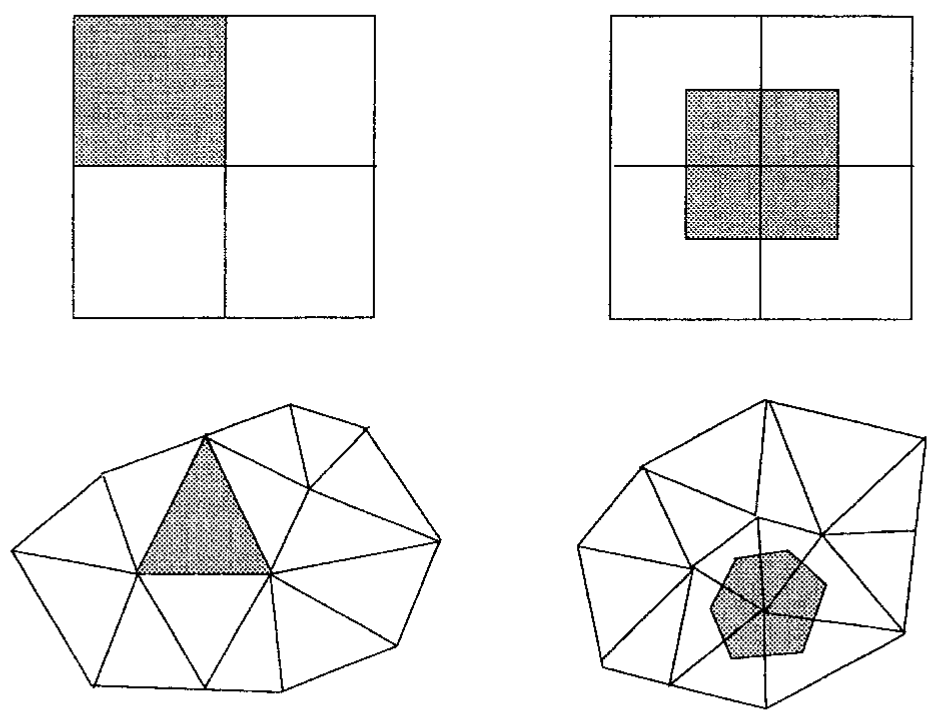
\includegraphics[width=.514\paperwidth]{images/fig-14-6-1.png}
  \caption{控制体积的例子}\label{fig:14.6.1}
\end{figure}

在\eqref{eq:14.6.8}中,下列选择会给出不同的离散形式：
\begin{enumerate}[label=\alph*.]
  \item 假定函数 \(\boldsymbol{w}\) 在 \(V_J\) 内所取的多项式形式.
  \item \(\boldsymbol{w}\) 的自由度.
  \item 边界通量的计算方式,即相邻控制体积之间的交换机制.
\end{enumerate}
通常,将\eqref{eq:14.6.8}中的体积分替换为
\begin{equation}\label{eq:14.6.9}
  \int_{V_J}\boldsymbol{\sigma}(\boldsymbol{w})\,\mathrm d\boldsymbol{x}
     \simeq(\boldsymbol{\sigma}(\boldsymbol{w}))_J\operatorname{meas}(V_J).
\end{equation}

\SourcePage{512}
这里,\((\boldsymbol{\sigma}(\boldsymbol{w}))_J\) 代表流动变量 \(\boldsymbol{\sigma}(\boldsymbol{w})\) 在控制体积 \(V_J\) 上的\emph{平均值}.若有源项,也采用同样的近似.

关于自由度的选择,可以采用\emph{单元中心}、\emph{单元顶点}或\emph{节点中心}逼近.矩形体积的情形见\figref{fig:14.6.2}.在单元中心有限体积法中,变量与单元关联,因而表示单元平均值,可以看成单元内某一点处的代表值.例如,对空间二阶的有限体积格式,可取单元的重心作为该点.单元顶点法和节点中心法都将变量与网格点关联.

在处理可压缩流动的 Euler 或 Navier--Stokes 方程等守恒律方程组时,可以用交错网格作有限体积离散.在这种情形下,不同物理未知量与不同的自由度关联.参见\BookCite{patankar1980}{Patankar(1980)}.

\begin{figure}[htbp]
  \centering
  \begin{subfigure}[t]{.202\paperwidth}
    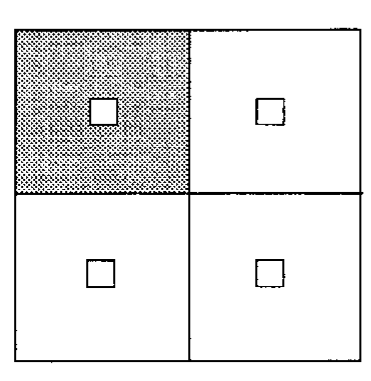
\includegraphics[width=\linewidth]{images/fig-14-6-2a.png}
    \caption{}\label{fig:14.6.2a}
  \end{subfigure}\hspace{.044\paperwidth}%
  \begin{subfigure}[t]{.216\paperwidth}
    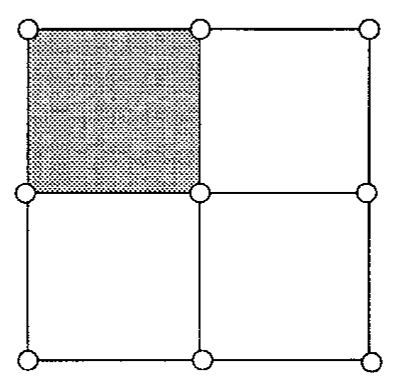
\includegraphics[width=\linewidth]{images/fig-14-6-2b.png}
    \caption{}\label{fig:14.6.2b}
  \end{subfigure}\hspace{.031\paperwidth}%
  \begin{subfigure}[t]{.216\paperwidth}
    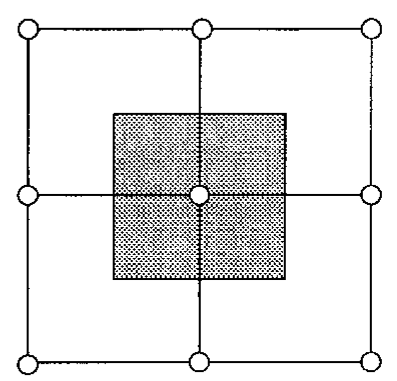
\includegraphics[width=\linewidth]{images/fig-14-6-2c.png}
    \caption{}\label{fig:14.6.2c}
  \end{subfigure}
  \caption{单元中心(a)、单元顶点(b)和节点中心(c)体积.阴影区域表示控制体积}\label{fig:14.6.2}
\end{figure}

就网格而言,有两类剖分：
\begin{enumerate}
  \item 类似有限差分网格,所有网格点都在两族线的交点上,例如两族分别平行于坐标轴的直线.这通常称为\emph{结构网格}.例子见\figref{fig:14.6.2}\subref{fig:14.6.2a}和\figref{fig:14.6.3}\subref{fig:14.6.3a}.
  \item 类似有限元网格,由三角形或四边形单元任意组合而成.网格点无法用一对整数来标识,需要逐点编号,并明确给出各顶点之间的连接关系.这类网格称为\emph{非结构网格}.例子见\figref{fig:14.6.2}\subref{fig:14.6.2b}和\figref{fig:14.6.3}\subref{fig:14.6.3b}.
\end{enumerate}
对于复杂几何构型,非结构网格更灵活.

采用结构网格,则很容易把计算区域映射为矩形区域.此外,将导数按各坐标线分开处理,便可将一维算法
\SourcePage{513}
推广到二维.结构网格也可以处理复杂几何,做法是把区域划分为多个块.

\begin{figure}[htbp]
  \centering
  \begin{subfigure}[t]{.315\paperwidth}
    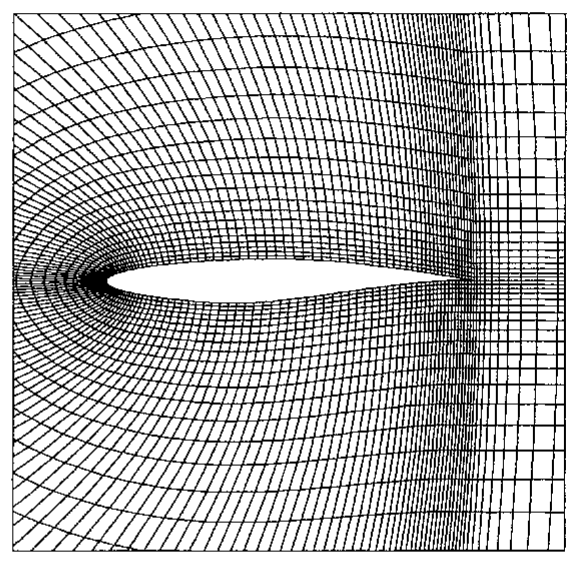
\includegraphics[width=\linewidth]{images/fig-14-6-3a.png}
    \caption{}\label{fig:14.6.3a}
  \end{subfigure}\hspace{.060\paperwidth}%
  \begin{subfigure}[t]{.312\paperwidth}
    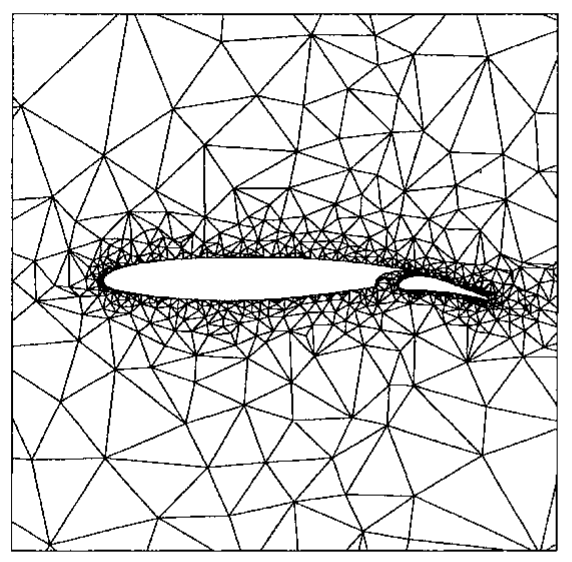
\includegraphics[width=\linewidth]{images/fig-14-6-3b.png}
    \caption{}\label{fig:14.6.3b}
  \end{subfigure}
  \caption{翼型周围的结构网格(a)和非结构网格(b)}\label{fig:14.6.3}
\end{figure}

在变量选取方面,单元中心离散常与结构网格配合使用.此时的难点是如何施加边界条件,因为代表单元值的网格点都不在区域边界 \(\partial\Omega\) 上.这一问题通常用外推法解决.节点中心法通常用于非结构网格.

有限体积法还有一个区别不同格式的关键方面,就是计算边界通量的策略.沿 \(\partial V_J\) 各边计算通量分量(见\eqref{eq:14.6.8})时,既要考虑所选格式,也要考虑流动变量的位置,即所选的自由度.基本上可以分为中心离散格式和迎风离散格式.

中心格式用对称的方式估计通量,计入界面两侧的贡献.这时需要在格式中人工加入适量的数值耗散,以防发生振荡.参见\BookCite{jameson-schmidt-turkel1981}{Jameson、Schmidt 和 Turkel(1981)}.

迎风格式根据各波分量的传播方向确定各边上的通量.下面简要讨论几个可用的准则.暂且不考虑黏性通量.第一种做法是在边 \(\Sigma\) 上,把法向通量 \(\boldsymbol{H}_{\rm inv}(\boldsymbol{w})\cdot\boldsymbol{n}=:\boldsymbol{H}_\Sigma(\boldsymbol{w})\) 换成依赖于两个状态(左、右或上、下)的数值通量函数 \(\boldsymbol{H}^{\rm num}(\boldsymbol{w}^l,\boldsymbol{w}^r)\).数值通量必须与精确通量一致,可以仿照第~\ref{sec:14.2.3}~节对一维标量双曲型方程的做法来选取.一种选法是先对前一时间层的两个状态 \(\boldsymbol{w}^l,\boldsymbol{w}^r\)
\SourcePage{514}
应用 Riemann 求解器,再计算 \(\boldsymbol{H}_\Sigma(\boldsymbol{w})\).例如,在结构网格上,可用第~\ref{sec:14.2.3}~节的有限差分逼近方式来实现.

也可采用更直接的做法.为简便起见,考虑\figref{fig:14.6.4}中的结构网格,它与单元中心有限体积法相对应.

设 \(V_J\) 为矩形 \(ABCD\),且 \(\boldsymbol{H}_{\rm inv}=(\boldsymbol{F}\mid\boldsymbol{G})\),其中 \(\boldsymbol{F},\boldsymbol{G}\) 是四维列向量,则
\begin{equation}\label{eq:14.6.10}
  \begin{aligned}
    \int_{\partial V_J}\boldsymbol{H}_{\rm inv}(\boldsymbol{w})\cdot\boldsymbol{n}\,\mathrm d\gamma
      &=\int_{AB}\boldsymbol{F}(\boldsymbol{w})\,\mathrm d\gamma
          +\int_{BC}\boldsymbol{G}(\boldsymbol{w})\,\mathrm d\gamma\\
      &\qquad-\int_{CD}\boldsymbol{F}(\boldsymbol{w})\,\mathrm d\gamma
          -\int_{DA}\boldsymbol{G}(\boldsymbol{w})\,\mathrm d\gamma,
  \end{aligned}
\end{equation}
其中各边上的 \(\mathrm d\gamma\) 均为正的弧长测度.在离散中,可用以下\emph{中心}格式逼近右端：
\begin{equation}\label{eq:14.6.11}
  \begin{aligned}
    &\boldsymbol{F}_{AB}|x_{B,2}-x_{A,2}|+\boldsymbol{G}_{BC}|x_{B,1}-x_{C,1}|\\
    &\qquad-\boldsymbol{F}_{CD}|x_{C,2}-x_{D,2}|
             -\boldsymbol{G}_{DA}|x_{A,1}-x_{D,1}|.
  \end{aligned}
\end{equation}
以 \(\boldsymbol{F}_{AB}\) 为例,可考虑几种选法.
\begin{enumerate}[label=\alph*.]
  \item 左右通量的平均：
    \begin{equation}\label{eq:14.6.12}
      \boldsymbol{F}_{AB}=\tfrac12(\boldsymbol{F}_{i+1,j}+\boldsymbol{F}_{i,j}),
      \qquad\boldsymbol{F}_{i,j}:=\boldsymbol{F}(\boldsymbol{w}_{i,j}),
    \end{equation}
    其中 \(\boldsymbol{w}_{i,j}\) 是 \(\boldsymbol{w}\) 在节点 \((i,j)\) 的值.
  \item 顶点通量的平均：
    \begin{equation}\label{eq:14.6.13}
      \boldsymbol{F}_{AB}=\tfrac12(\boldsymbol{F}_A+\boldsymbol{F}_B),
      \qquad\boldsymbol{F}_A:=\boldsymbol{F}(\boldsymbol{w}_A),\quad
            \boldsymbol{F}_B:=\boldsymbol{F}(\boldsymbol{w}_B),
    \end{equation}
    其中 \(\boldsymbol{w}_A\) 和 \(\boldsymbol{w}_B\) 分别是汇于点 \(A\) 和点 \(B\) 的四个单元上的 \(\boldsymbol{w}\) 值之和除以 \(4\).
  \item 变量平均后的通量：
    \begin{equation}\label{eq:14.6.14}
      \boldsymbol{F}_{AB}=\boldsymbol{F}\bigl(\tfrac12(\boldsymbol{w}_{i+1,j}+\boldsymbol{w}_{i,j})\bigr).
    \end{equation}
\end{enumerate}
其余通量也可类似计算.

对于单元顶点有限体积法,选法\eqref{eq:14.6.13}也很直接,不过此时 \(\boldsymbol{w}_A\) 和 \(\boldsymbol{w}_B\) 分别表示 \(\boldsymbol{w}\) 在顶点 \(A\) 和 \(B\) 的值.

不难看出,在均匀网格上,上述有限体积法实际上与有限差分格式一致.例如,若每个单元的大小为 \(\Delta x_1\times\Delta x_2\),选法\eqref{eq:14.6.12}导出二阶中心格式
\[
  \frac{\partial\boldsymbol{\sigma}(\boldsymbol{w}_{i,j})}{\partial t}
    +\frac{\boldsymbol{F}_{i+1,j}-\boldsymbol{F}_{i-1,j}}{2\Delta x_1}
    +\frac{\boldsymbol{G}_{i,j+1}-\boldsymbol{G}_{i,j-1}}{2\Delta x_2}=0.
\]

\SourcePage{515}
\begin{figure}[htbp]
  \centering
  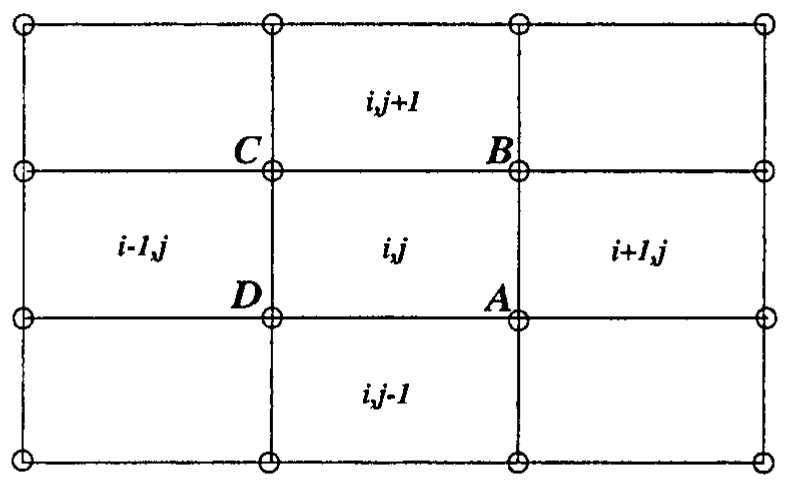
\includegraphics[width=.429\paperwidth]{images/fig-14-6-4.png}
  \caption{单元中心有限体积}\label{fig:14.6.4}
\end{figure}

如第~\ref{sec:14.2}~节所见,因此可以预期会发生振荡,这也提示我们在这里采用\emph{迎风}格式.也就是说,对流通量的计算取决于相应对流速度所决定的传播方向.对流速度由通量对守恒变量的 Jacob 矩阵给出.以 \(\boldsymbol{w}\) 表示守恒变量时,记为
\[
  A(\boldsymbol{w})=\frac{\partial\boldsymbol{H}_{\rm inv}(\boldsymbol{w})}{\partial\boldsymbol{w}}.
\]
对于给定的边,使用其法向通量的 Jacob 矩阵.

对于单元中心有限体积法,最简单的迎风格式令单元边通量等于上游单元所产生的通量.在均匀网格上,这给出标准的迎风有限差分格式.

对于单元顶点有限体积法,根据对流速度的符号,用 \(\boldsymbol{F}_{CD}\) 或 \(\boldsymbol{F}_{EF}\) 代替通量 \(\boldsymbol{F}_{AB}\).这里 \(EF\) 指 \(AB\) 右侧与它平行的下一条网格边.因此,所得格式的差分模板可能相当宽.

黏性通量,即\eqref{eq:14.6.8}中的 \(\int_{\partial V_J}\boldsymbol{H}_{\rm vis}(\boldsymbol{w})\cdot\boldsymbol{n}\,\mathrm d\gamma\),通常用中心格式计算.有时也采用有限元做法处理这些项,例如见\BookCite{rostand-stoufflet1988}{Rostand 和 Stoufflet(1988)}、\BookCite{tidriri1992}{Tidriri(1992)}及\BookCite{arminjon-dervieux1993}{Arminjon 和 Dervieux(1993)}.关于结构网格上可压缩 Navier--Stokes 方程的其他有限体积格式,见\BookCite{crumpton-mackenzie-morton1993}{Crumpton、Mackenzie 和 Morton(1993)}及其中的参考文献.

时间推进格式可以是显式的,也可以是隐式的.求定常解时,显式格式若配以适当的加速技术,也能有竞争力.这些技术包括局部时间步进、用于计算残差的多重网格技术,以及适当的残差光滑化.有关介绍,见\BookCite{johnson1983}{Johnson(1983)}、\BookCite{jameson1985}{Jameson(1985)}、\BookCite{koren1988}{Koren(1988)}、\BookCite{lallemand-koren1989}{Lallemand 和 Koren(1989)}、\BookCite{lallemand-steve-dervieux1992}{Lallemand、Steve 和 Dervieux(1992)}以及\BookCite{hemker-desideri1993}{Hemker 和 Desideri(1993)}.

对于非定常问题,隐式方法一般更高效,尤其是在高 Reynolds 数的黏性流动中.这些格式通常用所谓的增量形式实现,即每一步求解未知增量 \(\Delta\boldsymbol{w}^{(n)}:=\boldsymbol{w}^{n+1}-\boldsymbol{w}^n\).下面简述得到这一形式的办法.从\eqref{eq:14.6.1}出发,
\SourcePage{516}
用向后 Euler 格式推进时间,对每个控制体积 \(V_J\) 得到
\[
  \int_{V_J}\frac{\boldsymbol{\sigma}(\boldsymbol{w}^{n+1})-\boldsymbol{\sigma}(\boldsymbol{w}^n)}{\Delta t}
             \,\mathrm d\boldsymbol{x}
        +\int_{\partial V_J}\boldsymbol{\varphi}(\boldsymbol{w}^{n+1})\,\mathrm d\gamma=0.
\]
对含未知量的项作一阶 Taylor 展开,得到近似方程
\[
  \begin{aligned}
    &\frac1{\Delta t}\int_{V_J}
         \frac{\partial\boldsymbol{\sigma}}{\partial\boldsymbol{w}}(\boldsymbol{w}^n)
            \Delta\boldsymbol{w}^{(n)}\,\mathrm d\boldsymbol{x}
       +\int_{\partial V_J}\frac{\partial\boldsymbol{\varphi}}{\partial\boldsymbol{w}}(\boldsymbol{w}^n)
            \Delta\boldsymbol{w}^{(n)}\,\mathrm d\gamma\\
    &\qquad=-\int_{\partial V_J}\boldsymbol{\varphi}(\boldsymbol{w}^n)\,\mathrm d\gamma.
  \end{aligned}
\]
这可作为实现上述任一种有限体积格式的出发点.

\section{补充说明}\label{sec:14.7}

\BookCite{van-leer1992}{van Leer(1992)}综述了多维迎风有限差分法.\BookCite{coquel-lefloch1993}{Coquel 和 Le Floch(1993)}给出了一般收敛理论.

在有限元方面,非线性双曲型方程近年来得到了广泛研究.关于理论分析,可参见 Johnson 及其合作者的工作,例如\BookCite{johnson-szepessy1987}{Johnson 和 Szepessy(1987)}、\BookCite{johnson-szepessy-hansbo1990}{Johnson、Szepessy 和 Hansbo(1990)}和 Szepessy(\BookCite{szepessy1989}{1989}、\BookCite{szepessy1991}{1991}).关于在可压缩无黏流动中的数值应用,参见\BookCite{hughes-tezduyar1984}{Hughes 和 Tezduyar(1984)}、\BookCite{shakib1988}{Shakib(1988)}、\BookCite{lebeau-tezduyar1991}{Le Beau 和 Tezduyar(1991)}以及\BookCite{lebeau-ray-aliabadi-tezduyar1993}{Le Beau、Ray、Aliabadi 和 Tezduyar(1993)}.

有一种方法把有限元剖分的几何灵活性与类似有限差分的界面通量处理结合起来,后者采用类似 ENO 的做法.这便是\emph{间断 Galerkin--Runge--Kutta 法}的基础.相关的提出和分析见 Cockburn 和 Shu(\BookCite{cockburn-shu1989}{1989}、\BookCite{cockburn-shu1991}{1991})、\BookCite{cockburn-lin-shu1989}{Cockburn、Lin 和 Shu(1989)}以及\BookCite{cockburn-hou-shu1990}{Cockburn、Hou 和 Shu(1990)}.这种方法所得格式具有 TVB 性质.当用次数不超过 \(k\)(\(k\ge1\))的多项式定义有限元子空间时,格式具有 \(k\) 阶精度.

关于非线性双曲型方程的 Taylor--Galerkin 法综述,见\BookCite{donea-quartapelle1992}{Donea 和 Quartapelle(1992)}.
